\documentclass{amsart}
\usepackage[margin=1.1in]{geometry} 
\usepackage{amsmath}
\usepackage{tcolorbox}
\usepackage{amssymb}
\usepackage{amsthm}
\usepackage{lastpage}
\usepackage{fancyhdr}
\usepackage{accents}
\usepackage{hyperref}
\usepackage{xcolor}
\usepackage{color}
% Fields
\newcommand{\CC}{\mathbb{C}}
\newcommand{\RR}{\mathbb{R}}
\newcommand{\QQ}{\mathbb{Q}}
\newcommand{\ZZ}{\mathbb{Z}}
\newcommand{\NN}{\mathbb{N}}
\newcommand{\FF}{\mathbb{F}}
\newcommand{\PP}{\mathbb{P}}

% mathcal letters
\newcommand{\Acal}{\mathcal{A}}
\newcommand{\Bcal}{\mathcal{B}}
\newcommand{\Ccal}{\mathcal{C}}
\newcommand{\Dcal}{\mathcal{D}}
\newcommand{\Ecal}{\mathcal{E}}
\newcommand{\Fcal}{\mathcal{F}}
\newcommand{\Gcal}{\mathcal{G}}
\newcommand{\Hcal}{\mathcal{H}}
\newcommand{\Ical}{\mathcal{I}}
\newcommand{\Jcal}{\mathcal{J}}
\newcommand{\Kcal}{\mathcal{K}}
\newcommand{\Lcal}{\mathcal{L}}
\newcommand{\Mcal}{\mathcal{M}}
\newcommand{\Ncal}{\mathcal{N}}
\newcommand{\Ocal}{\mathcal{O}}
\newcommand{\Pcal}{\mathcal{P}}
\newcommand{\Qcal}{\mathcal{Q}}
\newcommand{\Rcal}{\mathcal{R}}
\newcommand{\Scal}{\mathcal{S}}
\newcommand{\Tcal}{\mathcal{T}}
\newcommand{\Ucal}{\mathcal{U}}
\newcommand{\Vcal}{\mathcal{V}}
\newcommand{\Wcal}{\mathcal{W}}
\newcommand{\Xcal}{\mathcal{X}}
\newcommand{\Ycal}{\mathcal{Y}}
\newcommand{\Zcal}{\mathcal{Z}}

% abstract categories
\newcommand{\Asf}{\mathsf{A}}
\newcommand{\Bsf}{\mathsf{B}}
\newcommand{\Csf}{\mathsf{C}}
\newcommand{\Dsf}{\mathsf{D}}
\newcommand{\Esf}{\mathsf{E}}
\newcommand{\Ssf}{\mathsf{S}}

% algebraic geometry
\newcommand{\spec}{\operatorname{Spec}}
\newcommand{\proj}{\operatorname{Proj}}

% categories 
\newcommand{\id}{\mathrm{id}}
\newcommand{\Obj}{\mathrm{Obj}}
\newcommand{\Mor}{\mathrm{Mor}}
\newcommand{\Hom}{\mathrm{Hom}}
\newcommand{\Aut}{\mathrm{Aut}}
\newcommand{\Sets}{\mathsf{Sets}}
\newcommand{\SSets}{\mathsf{SSets}}
\newcommand{\kVec}{\mathsf{Vec}_{k}}
\newcommand{\Alg}{\mathsf{Alg}}
\newcommand{\Ring}{\mathsf{Ring}}
\newcommand{\Mod}{\mathsf{Mod}}
\newcommand{\Grp}{\mathsf{Grp}}
\newcommand{\AbGrp}{\mathsf{AbGrp}}
\newcommand{\PSh}{\mathsf{PSh}}
\newcommand{\Sh}{\mathsf{Sh}}
\newcommand{\PSch}{\mathsf{PSch}}
\newcommand{\Sch}{\mathsf{Sch}}
\newcommand{\Top}{\mathsf{Top}}
\newcommand{\Com}{\mathsf{Com}}
\newcommand{\Coh}{\mathsf{Coh}}
\newcommand{\QCoh}{\mathsf{QCoh}}
\newcommand{\Opens}{\mathsf{Opens}}
\newcommand{\Opp}{\mathsf{Opp}}
\newcommand{\Cat}{\mathsf{Cat}}
\newcommand{\NatTrans}{\mathrm{NatTrans}}
\newcommand{\pr}{\mathrm{pr}}
\newcommand{\Fun}{\mathrm{Fun}}
\newcommand{\colim}{\mathrm{colim}}
\newcommand{\lifts}{\boxslash}
\DeclareMathOperator\squarediv{\lifts}

% simplicial sets
\newcommand{\DDelta}{\Updelta}
\newcommand{\Sing}{\operatorname{Sing}}

% ideal theory
\newcommand{\mfrak}{\mathfrak{m}}
\newcommand{\afrak}{\mathfrak{a}}
\newcommand{\bfrak}{\mathfrak{b}}
\newcommand{\pfrak}{\mathfrak{p}}
\newcommand{\qfrak}{\mathfrak{q}}

% number theory
\newcommand{\Tr}{\mathrm{Tr}}
\newcommand{\Nm}{\mathrm{Nm}}
\newcommand{\Gal}{\mathrm{Gal}}
\newcommand{\Frob}{\mathrm{Frob}}
\setlength{\headheight}{40pt}


\newenvironment{solution}
  {\renewcommand\qedsymbol{$\blacksquare$}
  \begin{proof}[Solution]}
  {\end{proof}}
\renewcommand\qedsymbol{$\blacksquare$}

\usepackage{amsmath, amssymb, tikz, amsthm, csquotes, multicol, footnote, tablefootnote, biblatex, wrapfig, float, quiver, mathrsfs, cleveref, enumitem, upgreek,stmaryrd}
\addbibresource{refs.bib}
\theoremstyle{definition}
\newtheorem{theorem}{Theorem}[section]
\newtheorem{lemma}[theorem]{Lemma}
\newtheorem{corollary}[theorem]{Corollary}
\newtheorem{exercise}[theorem]{Exercise}
\newtheorem{question}[theorem]{Question}
\newtheorem{example}[theorem]{Example}
\newtheorem{proposition}[theorem]{Proposition}
\newtheorem{conjecture}[theorem]{Conjecture}
\newtheorem*{remark}{Remark}
\newtheorem{definition}[theorem]{Definition}
\numberwithin{equation}{section}
\begin{document}
\large
\title[Infinity Categories]{MATH 292Z: First Steps in Infinity Categories}
\author{Wern Juin Gabriel Ong}
\address{Bowdoin College, Brunswick, Maine 04011}
\email{gong@bowdoin.edu}
\urladdr{https://wgabrielong.github.io/}
\maketitle
\section*{Preliminaries}
These notes roughly correspond to the course \textbf{MATH 292Z: First Steps in Infinity Categories} taught by Prof. Michael Hopkins at Harvard University in the Fall 2023 semester. These notes are \LaTeX-ed after the fact with significant alteration and are subject to misinterpretation and mistranscription. Use with caution. Any errors are undoubtedly my own and any virtues that could be ascribed to these notes ought be attributed to the instructor and not the typist. A special thanks to Prof. Hopkins, who made his lecture notes available to the class, and in referencing it have greatly improved my own notes and understanding of the subject. 
\tableofcontents
\include{Lecture 1}
\section{Lecture 2 -- 11th September 2023}
We made a very quick pass of simplicial sets in the previous lecture. Let us go through it in more detail. 

Let $\DDelta$ be the category whose objects are finite ordered sets and whose morphisms are order-preserving maps. Following the notation in Rezk's text \cite{Rezk}, for a morphism $[n]\to[k]$, we write it $\langle k_{0},\dots,k_{n}\rangle$ where $0\leq k_{0}\leq\dots\leq k_{n}\leq k$. In the category $\DDelta$, there are two types of distinguished maps $d_{i}$ and $s_{i}$ which we now define. 
\begin{definition}[Face Maps]\label{def:face maps}
  In the category $\DDelta$, there are maps $d^{k}:[n-1]\to[n]$ by $\langle 0,1,\dots,\hat{k},\dots,n\rangle=\langle 0,1,\dots,k-1,k+1,\dots,n\rangle\to[n]$. 
\end{definition}
\begin{example}
  We should think of these as the inclusion of a face into the simplex. 
  $$% https://q.uiver.app/#q=WzAsNyxbMiwyLCIxIl0sWzQsMiwiMCJdLFs2LDMsIjEiXSxbNiwxLCIyIl0sWzUsMCwiMyJdLFswLDEsIjAiXSxbMiwwLCIyIl0sWzIsNF0sWzEsMl0sWzIsM10sWzEsNF0sWzEsM10sWzMsNF0sWzUsMF0sWzAsNl0sWzUsNl0sWzE0LDcsImReezJ9IiwwLHsiY3VydmUiOjEsInNob3J0ZW4iOnsic291cmNlIjoyMCwidGFyZ2V0IjoyMH19XV0=
  \begin{tikzcd}
    && 2 &&& 3 \\
    0 &&&&&& 2 \\
    && 1 && 0 \\
    &&&&&& 1
    \arrow[""{name=0, anchor=center, inner sep=0}, from=4-7, to=1-6]
    \arrow[from=3-5, to=4-7]
    \arrow[from=4-7, to=2-7]
    \arrow[from=3-5, to=1-6]
    \arrow[from=3-5, to=2-7]
    \arrow[from=2-7, to=1-6]
    \arrow[from=2-1, to=3-3]
    \arrow[""{name=1, anchor=center, inner sep=0}, from=3-3, to=1-3]
    \arrow[from=2-1, to=1-3]
    \arrow["{d^{2}}", curve={height=6pt}, shorten <=23pt, shorten >=23pt, rightarrow, from=1, to=0]
  \end{tikzcd}$$
  Here, we show the inclusion $d^{2}:[2]\to[3]$ by $\langle0,1,3\rangle$, taking the 2-simplex to the face ``opposite'' the vertex 2, that is, the face bounded by the vertices 0, 1, and 3. 
\end{example}
We can also define degeneracy maps as follows. 
\begin{definition}[Degeneracy Map]\label{def:degeneracy map}
  In the category $\DDelta$, there are maps $s^{k}:[n]\to[n-1]$ by $[n]\mapsto\langle 0,1,2,\dots,k,k,k+1,\dots,n\rangle$. 
\end{definition}
\begin{example}
  We should think of this as collapsing the $k$th to the $(k-1)$th vertex. 
  $$% https://q.uiver.app/#q=WzAsNixbMCwwLCIxIl0sWzAsMV0sWzAsMiwiMCJdLFsyLDEsIjIiXSxbMCw0LCIwIl0sWzIsNCwiMSJdLFswLDNdLFsyLDNdLFsyLDBdLFs0LDVdLFs3LDksInNeezB9IiwwLHsiY3VydmUiOi0xLCJzaG9ydGVuIjp7InNvdXJjZSI6MTAsInRhcmdldCI6MTB9fV1d
  \begin{tikzcd}
    1 \\
    {} && 2 \\
    0 \\
    \\
    0 && 1
    \arrow[from=1-1, to=2-3]
    \arrow[""{name=0, anchor=center, inner sep=0}, from=3-1, to=2-3]
    \arrow[from=3-1, to=1-1]
    \arrow[""{name=1, anchor=center, inner sep=0}, from=5-1, to=5-3]
    \arrow["{s^{0}}", curve={height=-6pt}, shorten <=5pt, shorten >=5pt, rightarrow, from=0, to=1]
  \end{tikzcd}$$
  Here we show $s^{0}:[2]\to[1]$ by $\langle 0,0,1\rangle$ collapsing the vertex 1 to the vertex 0. 
\end{example}
With these operations on $\DDelta$, one can in fact show the following theorem. 
\begin{theorem}
  If $f$ is a morphism in $\DDelta$, then $f$ factors as the composition of face and degeneracy maps. 
\end{theorem}
We omit the proof. 

Now recall that a simplicial set $X$ is a covariant functor $X:\DDelta^{\Opp}\to\Sets$. We write $$X_{n}=\Fun([n], X)
.$$ For a simplicial set $X$, we have a diagram
$$% https://q.uiver.app/#q=WzAsNSxbMCwwLCJYX3swfSJdLFsyLDAsIlhfezF9Il0sWzQsMCwiWF97Mn0iXSxbNSwwLCJcXGRvdHMiXSxbNiwwLCJcXGRvdHMiXSxbMCwxLCJzXnswfSIsMV0sWzEsMCwiZF57MX0iLDEseyJvZmZzZXQiOi0zLCJjdXJ2ZSI6LTF9XSxbMCwxLCJkXnswfSIsMSx7Im9mZnNldCI6LTMsImN1cnZlIjotMSwic3R5bGUiOnsidGFpbCI6eyJuYW1lIjoiYXJyb3doZWFkIn0sImhlYWQiOnsibmFtZSI6Im5vbmUifX19XSxbMSwyLCJzXnsxfSIsMSx7Im9mZnNldCI6MywiY3VydmUiOjF9XSxbMiwxLCJkXnsxfSIsMV0sWzEsMiwic157MH0iLDEseyJvZmZzZXQiOi0yLCJjdXJ2ZSI6LTF9XSxbMiwxLCJkXnsyfSIsMSx7Im9mZnNldCI6LTUsImN1cnZlIjotMn1dLFsyLDEsImReezB9IiwxLHsib2Zmc2V0Ijo1LCJjdXJ2ZSI6Mn1dXQ==
\begin{tikzcd}
	{X_{0}} && {X_{1}} && {X_{2}} & \dots & \dots
	\arrow["{s^{0}}"{description}, from=1-1, to=1-3]
	\arrow["{d^{1}}"{description}, shift left=3, curve={height=-6pt}, from=1-3, to=1-1]
	\arrow["{d^{0}}"{description}, shift left=3, curve={height=-6pt}, tail reversed, no head, from=1-1, to=1-3]
	\arrow["{s^{1}}"{description}, shift right=3, curve={height=6pt}, from=1-3, to=1-5]
	\arrow["{d^{1}}"{description}, from=1-5, to=1-3]
	\arrow["{s^{0}}"{description}, shift left=2, curve={height=-6pt}, from=1-3, to=1-5]
	\arrow["{d^{2}}"{description}, shift left=5, curve={height=-12pt}, from=1-5, to=1-3]
	\arrow["{d^{0}}"{description}, shift right=5, curve={height=12pt}, from=1-5, to=1-3]
\end{tikzcd}$$
induced by the degeneracy and face maps. 
\begin{definition}[$n$-Simplex]
  The $n$-simplex is the functor $\Delta^{n}:\DDelta^{\Opp}\to\Sets$ by $[k]\mapsto\Mor_{\DDelta}([k],[n])$. 
\end{definition}
\begin{remark}
  Note that $\Delta^{n}$ is the functor $\DDelta^{\Opp}\to\Sets$, while the topological $n$-simplex $|\Delta^{n}|\simeq S^{n}\in\Obj(\Top)$ is topological space homeomorphic (and homotopic) to the $n$-sphere. 
\end{remark}
In this way, we can think of $\Delta^{n}$ as the functor represented by $[n]\in\Obj(\DDelta)$. More generally, one can define representable functors as follows. 
\begin{definition}[Representable Functor]
  Let $\Csf$ be a category. A functor $F:\Csf\to\Sets$ is representable if there exists $A\in\Obj(\Csf)$ such that there exists an isomorphism of functors $F\to\Mor_{\Csf}(-,A)$. 
\end{definition}
Generally, consider $F:\Csf^{\Opp}\to\Sets$ a contravariant functor from an arbitrary category $\Csf$ to $\Sets$. Let $f:B\to A$. $F(f):F(B)\to F(A)$ is a map betewen sets. For $u\in F(A)$, $u$ determines a natural transformation of functors $\NatTrans(\Mor_{\Csf}(-,A),F)$. This is Yoneda's lemma. We adapt the version from \cite[Theorem 2.2.4]{Riehl}.  
\begin{lemma}[Yoneda]\label{lem:yoneda}
  For a contravariant functor $F:\Csf\to\Sets$ and $A\in\Obj(\Csf)$, there is a bijection 
  $$\NatTrans(\Mor_{\Csf}(-,A), F)\to F(A)$$
  that associates a natural transformation of functors $\alpha:\Mor_{\Csf}(-,A)\Rightarrow F$ to the element $\alpha(\id_{A})\in F(A)$, natural in both $A$ and $F$. 
\end{lemma}
Let us recall the definition of quasicategories as in \Cref{def:quasicategory}. 
\begin{definition}[Quasicategory]
  A simplcial set $X$ is a quasicategory if every inner horn $\Lambda^{n}_{k}$ where $0<k<n$ has a fill. 
\end{definition}
In other words, for every solid diagram, 
$$% https://q.uiver.app/#q=WzAsMyxbMCwwLCJcXExhbWJkYV57bn1fe2t9Il0sWzAsMSwiXFxEZWx0YV57bn0iXSxbMiwwLCJYIl0sWzAsMSwiIiwxLHsic3R5bGUiOnsidGFpbCI6eyJuYW1lIjoiaG9vayIsInNpZGUiOiJib3R0b20ifX19XSxbMCwyXSxbMSwyLCJcXGV4aXN0cyIsMSx7InN0eWxlIjp7ImJvZHkiOnsibmFtZSI6ImRhc2hlZCJ9fX1dXQ==
\begin{tikzcd}
	{\Lambda^{n}_{k}} && X \\
	{\Delta^{n}}
	\arrow[hook', from=1-1, to=2-1]
	\arrow[from=1-1, to=1-3]
	\arrow["\exists"{description}, dashed, from=2-1, to=1-3]
\end{tikzcd}$$
there is a dotted map making the diagram commute. 

Let us now fix some notation that we will use going forward. For $X$ a simplicial set we denote $X_{n}=\Fun([n],X)$ and $\alpha\in\Mor_{\DDelta}([k],[n])$, we have $X_{\alpha}:X_{n}\to X_{k}$. 
\begin{theorem}\label{thm: nerve iff unique filler}
  A simplicial set is the nerve of some category if and only if every inner horn has a unique filler. 
\end{theorem}
In other words, for every solid diagram, 
$$% https://q.uiver.app/#q=WzAsMyxbMCwwLCJcXExhbWJkYV57bn1fe2t9Il0sWzAsMSwiXFxEZWx0YV57bn0iXSxbMiwwLCJYIl0sWzAsMSwiIiwxLHsic3R5bGUiOnsidGFpbCI6eyJuYW1lIjoiaG9vayIsInNpZGUiOiJib3R0b20ifX19XSxbMCwyXSxbMSwyLCJcXGV4aXN0cyEiLDEseyJzdHlsZSI6eyJib2R5Ijp7Im5hbWUiOiJkYXNoZWQifX19XV0=
\begin{tikzcd}
	{\Lambda^{n}_{k}} && X \\
	{\Delta^{n}}
	\arrow[hook', from=1-1, to=2-1]
	\arrow[from=1-1, to=1-3]
	\arrow["{\exists!}"{description}, dashed, from=2-1, to=1-3]
\end{tikzcd}$$
there is a dotted map making the diagram commute. 

We omit the proof of \Cref{thm: nerve iff unique filler} which can be found in \cite[\S 1.7.10]{Rezk}. 

We want to consider an analogue of \Cref{thm: nerve iff unique filler} in the case of quasicategories. Let $X$ be a quasicategory with objects $X_{0}$ and morphisms $X_{1}$. For $f\in X_{0}$, let $\langle0\rangle^{*}f$ denote the source of the map $f$ and $\langle1\rangle^{*}f$ its target. Let 
$$% https://q.uiver.app/#q=WzAsMyxbMCwwLCJBIl0sWzAsMSwiQiJdLFsyLDAsIkMiXSxbMSwyLCJnIiwyXSxbMCwxLCJmIiwyXV0=
\begin{tikzcd}
	A && C \\
	B
	\arrow["g"', from=2-1, to=1-3]
	\arrow["f"', from=1-1, to=2-1]
\end{tikzcd}$$
be the image of a horn $\Lambda^{2}_{1}$ and $h=\tau\langle0,2\rangle:A\to C$ be the fill. 
$$% https://q.uiver.app/#q=WzAsMyxbMCwwLCJBIl0sWzAsMSwiQiJdLFsyLDAsIkMiXSxbMSwyLCJnIiwyXSxbMCwxLCJmIiwyXSxbMCwyLCJcXHRhdVxcbGFuZ2xlMCwyXFxyYW5nbGU9aCJdXQ==
\begin{tikzcd}
	A && C \\
	B
	\arrow["g"', from=2-1, to=1-3]
	\arrow["f"', from=1-1, to=2-1]
	\arrow["{\tau\langle0,2\rangle=h}", from=1-1, to=1-3]
\end{tikzcd}$$
Since the fill is not unique, we say $\tau$ witnesses $h$ as the composition of $g$ with $f$. This begs the question of how we can perform some operation to make $X$ into a category. This is done via the construction of the fundamental category, which can be done on simplicial sets in general. 
\begin{definition}[Fundamental Category]
  Let $X$ be a simplicial set. A category $\Csf$ is the fundamental category of $X$ if every map $X\to\Dsf$ for $\Dsf$ factors through $\Csf$ and $\Csf$ is final with respect to that property. 
\end{definition}
Fundamental categories are in general hard to construct, but much easier in the case of quasicategories. Indeed if $X$ is a quasicategory, its fundamental category coincides with its homotopy category $hX$. The homotopy category will have objects $X_{0}$ and morphisms those in $X_{1}$ up to ``witnessing''-equivalence. We will have to discuss these notions of equivalence before defining the homotopy category rigorously. 
\begin{definition}[Left-Equivalence]\label{def:left equivalence}
  Let $f,g\in\Mor_{X}(A,B)$. We say that $f$ is left-equivalent to $g$ if there is $\tau\in X_{2}$ such that $\tau\langle0,1\rangle=\id_{A}, \tau\langle0,2\rangle=f, \tau\langle1,2\rangle=g$. 
  $$% https://q.uiver.app/#q=WzAsMyxbMCwwLCJBIl0sWzAsMSwiQSJdLFsyLDEsIkIiXSxbMCwyLCJmIiwxXSxbMSwyLCJnIiwxXSxbMCwxLCJcXGlkX3tBfSIsMV1d
  \begin{tikzcd}
    A \\
    A && B
    \arrow["f"{description}, from=1-1, to=2-3]
    \arrow["g"{description}, from=2-1, to=2-3]
    \arrow["{\id_{A}}"{description}, from=1-1, to=2-1]
  \end{tikzcd}$$
\end{definition}
Similarly, we have right-equivalence. 
\begin{definition}[Right-Equivalence]\label{def:right equivalence}
  Let $f,g\in\Mor_{X}(A,B)$. We say that $f$ is right-equivalent to $g$ if there is $\tau\in X_{2}$ such that $\tau\langle1,2\rangle=\id_{B}, \tau\langle0,1\rangle=f, \tau\langle0,2\rangle=g$. 
  $$% https://q.uiver.app/#q=WzAsMyxbMCwxLCJBIl0sWzIsMSwiQiJdLFsyLDAsIkIiXSxbMCwyLCJnIiwxXSxbMSwyLCJcXGlkX3tCfSIsMV0sWzAsMSwiZiIsMV1d
  \begin{tikzcd}
    && B \\
    A && B
    \arrow["g"{description}, from=2-1, to=1-3]
    \arrow["{\id_{B}}"{description}, from=2-3, to=1-3]
    \arrow["f"{description}, from=2-1, to=2-3]
  \end{tikzcd}$$
\end{definition}
One then shows the following proposition before defining the homotopy category. 
\begin{proposition}\label{prop: left eq right equivalence}
  The relations of left equivalence (\Cref{def:left equivalence}) and right equivalence (\Cref{def:right equivalence}) coincide. 
\end{proposition}
We can now define the homotopy category. 
\begin{definition}[Homotopy Category]\label{def:homotopy category}
  Let $X$ be a simplicial set. The homotopy category $hX$ has objects those in $X_{0}$ and morphisms those in $X_{1}$ up to equivalence. 
\end{definition}
\section{Lecture 3 -- 13th September 2023}
We will discuss some constructions in ordinary category theory. Thinking about these constructions will give us a better idea of analogous constructions in infinity category theory. 
\begin{definition}[Isomorphism]\label{def:isomorphism}
  Let $\Csf$ be a category. A morphism $f\in\Mor_{\Csf}(A,B)$ is an isomorphism if there exists $g\in\Mor_{\Csf}(B,A)$ such that $g\circ f=\id_{A}$ and $f\circ g=\id_{B}$.
\end{definition}
One can easily show that isomorphisms are preserved by functors. 
\begin{proposition}
  Let $F:\Csf\to\Dsf$ be a functor. If $f\in\Mor_{\Csf}(A,B)$ is an isomorphism then $F(f)\in\Mor_{\Dsf}(F(A),F(B))$ is an isomorphism. 
\end{proposition}
\begin{proof}
  The statement follows by the commutativity of the following diagram. 
  $$% https://q.uiver.app/#q=WzAsNCxbMCwwLCJBIl0sWzIsMCwiQiJdLFswLDEsIkYoQSkiXSxbMiwxLCJGKEIpIl0sWzEsMywiRiIsMl0sWzAsMiwiRiIsMl0sWzAsMSwiZiIsMCx7Im9mZnNldCI6LTF9XSxbMSwwLCJnIiwwLHsib2Zmc2V0IjotMX1dLFsyLDMsIkYoZikiLDAseyJvZmZzZXQiOi0xfV0sWzMsMiwiRihnKSIsMCx7Im9mZnNldCI6LTF9XV0=
  \begin{tikzcd}
    A && B \\
    {F(A)} && {F(B)}
    \arrow["F"', from=1-3, to=2-3]
    \arrow["F"', from=1-1, to=2-1]
    \arrow["f", shift left, from=1-1, to=1-3]
    \arrow["g", shift left, from=1-3, to=1-1]
    \arrow["{F(f)}", shift left, from=2-1, to=2-3]
    \arrow["{F(g)}", shift left, from=2-3, to=2-1]
  \end{tikzcd}$$
  More explicitly, there exists $g\in\Mor_{\Csf}(B,A)$ such that $g\circ f=\id_{A}$ and $f\circ g=\id_{B}$ so by functoriality we have $F(g)\circ F(f)=\id_{F(A)},F(f)\circ F(g)=\id_{F(B)}$ as desired. 
\end{proof}
The acute would percieve that \Cref{def:isomorphism} may be slightly problematic since it involves some choice of $g\in\Mor_{\Csf}(B,A)$. The following proposition resolves this issue, showing that such a choice is unique. 
\begin{proposition}
  Let $\Csf$ be a category and $f\in\Mor_{\Csf}(A,B)$ is an isomorphism. If $g_{1},g_{2}\in\Mor_{\Csf}(B,A)$ satisfies $g_{i}\circ f=\id_{A}$ and $f\circ g_{i}=\id_{B}$ for $i\in\{1,2\}$ then $g_{1}=g_{2}$. 
\end{proposition}
\begin{proof}
  We have $g_{1}=g_{1}\circ\id_{Y}=g_{1}\circ f\circ g_{2}=\id_{X}\circ g_{2}=g_{2}$. 
\end{proof}
In some settings, it can be difficult to find such $g$ that satisfies the composition identities as set out in \Cref{def:isomorphism}. Fortunately, we can use the Yoneda functors from \Cref{lem:yoneda} to characterize isomorphisms. 
\begin{theorem}[Representable Functors Determine Isomorphism]\label{thm:rep functors determine iso}
  Let $\Csf$ be a category. A map $f:A\to B$ is an isomorphism if and only if there is an isomorphic natural transformation of the functors they represent $\Mor_{\Csf}(-,A)\to\Mor_{\Csf}(-,B)$.
\end{theorem}
\begin{remark}
  It is equivalent to require that for all $Z\in\Obj(\Csf)$, $\Mor_{\Csf}(Z,A)=\Mor_{\Csf}(Z,B)$. 
\end{remark}
\begin{proof}[Proof of \Cref{thm:rep functors determine iso}]
  This follows from the Yoneda lemma, \Cref{lem:yoneda}.  
\end{proof}
Note the increasing levels of abstraction we have encountered. We started with the ``traditional'' definition of isomorphism that one encounters in say a course on the theory of groups, followed by the characterization of isomorphisms via representable functors. Let us look at one more characterization of isomorphisms in the flavor of how we defined the objects of a category as the 0th nerve $(N\Csf)_{0}$, we can define a category $I_{\cong}$ with two objects and two non-identity morphisms
$$% https://q.uiver.app/#q=WzAsMixbMCwwLCIqIl0sWzIsMCwiKiJdLFswLDEsIiIsMCx7Im9mZnNldCI6LTF9XSxbMSwwLCIiLDAseyJvZmZzZXQiOi0xfV1d
\begin{tikzcd}
	{*} && {*}
	\arrow[shift left, from=1-1, to=1-3]
	\arrow[shift left, from=1-3, to=1-1]
\end{tikzcd}$$
and define an isomorphism as follows:
\begin{definition}[Isomorphism]
  Let $\Csf$ be a category. An isomorphism in $\Csf$ is a functor $I_{\cong}\to\Csf$. 
\end{definition}
We will no doubt revisit isomorphisms in the infinity categorical setting later in the course. 

Now, let us recall the following definitions. 
\begin{definition}[Initial Object]\label{def:initial object}
  Let $\Csf$ be a category. An object $X\in\Obj(\Csf)$ is initial if for all $Y\in\Obj(\Csf)$, there is a unique map $X\to Y$. 
\end{definition}
\begin{definition}[Final Object]\label{def:final object}
  Let $\Csf$ be a category. An object $X\in\Obj(\Csf)$ is final if for all $Y\in\Obj(\Csf)$, there is a unique map $Y\to X$. 
\end{definition}
We now show that final objects (and initial objects, by taking the opposite category) are unique up to unique isomorphism. In other words, they satisfy a universal property. Universal properties are ubiquitous in many fields of mathematics and significantly streamlines one's thinking about mathematical constructions. 
\begin{proposition}
  If $X_{1},X_{2}$ be final objects of a category $\Csf$ then $X_{1}$ is isomorphic to $X_{2}$. 
\end{proposition}
\begin{proof}
  Both $X_{1}$ and $X_{2}$ represent the same functor $\Csf\to\Sets$, taking any object of $\Csf$ to the one-point set $\{*\}$. 
\end{proof}
We have already seen how isomorphisms work in a category. We now define them in the setting of quasicategories. 
\begin{definition}[Isomorphism in Quasicategories]
  Let $X$ be a quasicategory. A morphism $f\in X_{1}$ is an isomorphism if and only if $[f]\in(hX)_{1}$ is an isomorphism. 
\end{definition}
Isomorphisms arising in homotopy categories will soon provide a tool for characterizing Kan complexes. We begin by defining the groupoid. 
\begin{definition}[Groupoid]\label{def:groupoid}
  A category $\Csf$ is a groupoid if all morphisms in $\Csf$ are isomorphisms. 
\end{definition}
\begin{example}
  The fundamental groupoid of a topological space $\Pi_{\leq1}X$ is a groupoid. Morphisms correspond to paths, which are invertible by sending $\gamma(t)\to\gamma(1-t)$. 
\end{example}
The following theorem outlines a correspondence between quasicategories and Kan complexes with the language of groupoids. 
\begin{theorem}\label{thm:kan complex iff hX groupoid}
  A quasicategory $X$ is a Kan complex if and only if its homotopy category $hX$ is a groupoid. 
\end{theorem}
\begin{proof}[Partial Proof of \Cref{thm:kan complex iff hX groupoid}]
  $(\Longrightarrow)$ We prove that if $X$ is a Kan complex, its homotopy category is a groupoid.  
  $$% https://q.uiver.app/#q=WzAsMyxbMCwxLCJBIl0sWzIsMSwiQiJdLFswLDAsIkEiXSxbMCwxLCJmIiwyXSxbMSwyLCJcXGV4aXN0cyEiLDIseyJzdHlsZSI6eyJib2R5Ijp7Im5hbWUiOiJkYXNoZWQifX19XSxbMCwyLCJcXGlkX3tBfSJdXQ==
  \begin{tikzcd}
    A \\
    A && B
    \arrow["f"', from=2-1, to=2-3]
    \arrow["{\exists}"', dashed, from=2-3, to=1-1]
    \arrow["{\id_{A}}", from=2-1, to=1-1]
  \end{tikzcd}$$
  Let $f:A\to B$ be a morphism in $X$ and since $X$ is a Kan complex, the horn $\Lambda^{2}_{0}$ admits a fill by some $\tau\in X_{2}$. One verifies that for $g=\tau\langle1,2\rangle$ we have $g\circ f=\id_{A}$. To show $f\circ g=\id_{B}$ we construct the diagram 
  $$% https://q.uiver.app/#q=WzAsMyxbMCwxLCJBIl0sWzIsMSwiQiJdLFsyLDAsIkIiXSxbMSwyLCJcXGlkX3tCfSIsMl0sWzAsMiwiZiJdLFsxLDAsIlxcZXhpc3RzIiwwLHsic3R5bGUiOnsiYm9keSI6eyJuYW1lIjoiZGFzaGVkIn19fV1d
  \begin{tikzcd}
    && B \\
    A && B
    \arrow["{\id_{B}}"', from=2-3, to=1-3]
    \arrow["f", from=2-1, to=1-3]
    \arrow["\exists", dashed, from=2-3, to=2-1]
  \end{tikzcd}$$
  and by the fact that $X$ is a Kan complex, the horn $\Lambda^{2}_{2}$ admits a fill by some $\tau'\in X_{2}$ such that $\tau'\langle0,1\rangle=h$ satisfying $f\circ h=\id_{B}$. But we have $g=g\circ \id_{B}=g\circ f\circ h=\id_{A}\circ h=h$ proving that there is a unique inverse in the homotopy category. 
\end{proof}
The converse, showing that a homotopy category in which all morphisms are isomorphisms arises as the homotopy category of a Kan complex is much more difficult requiring a significant combinatorial assertion. We will return to Joyal's proof of the converse later in this course. 
\begin{definition}[Quasigroupoid]
  A quasicategory $X$ is a quasigroupoid if $hX$ is a groupoid. 
\end{definition}
As \Cref{thm:kan complex iff hX groupoid} shows, Kan complexes are examples of quasigroupoids. 

\begin{definition}[Small Category]
  A category $\Csf$ is a small category if $\Obj(\Csf)$ is a set as opposed to a class. 
\end{definition}
Having defined a small category, we can define the category of small categories. 
\begin{definition}[Category of Small Categories]
  Denote $\Cat_{1}$ the category of small categories whose objects are small categories and whose morphisms are functors betweeen them. 
\end{definition}
Analogously to nerves, we can consider $(\Cat_{1})_{n}$ be the data of a category $\Csf_{i}$ for each $1\leq i\leq n$, a functor $F_{ij}:\Csf_{i}\to\Csf_{j}$ for each $i\leq j$, and a natural isomorphism of functors $\varepsilon_{ijk}:F_{ik}\Rightarrow F_{jk}\circ F_{ij}$ making the following diagram commute. 
$$% https://q.uiver.app/#q=WzAsNCxbMCwxLCJcXENzZl97aX0iXSxbMywxXSxbNCwxLCJcXENzZl97a30iXSxbMiwwLCJcXENzZl97an0iXSxbMCwzLCJGX3tpan0iXSxbMywyLCJGX3tqa30iXSxbMCwyLCJGX3tpa30iLDJdLFs2LDMsIlxcdmFyZXBzaWxvbl97aWprfSIsMCx7Im9mZnNldCI6LTEsInNob3J0ZW4iOnsic291cmNlIjoxMCwidGFyZ2V0IjozMH19XV0=
\begin{tikzcd}
	&& {\Csf_{j}} \\
	{\Csf_{i}} &&& {} & {\Csf_{k}}
	\arrow["{F_{ij}}", from=2-1, to=1-3]
	\arrow["{F_{jk}}", from=1-3, to=2-5]
	\arrow[""{name=0, anchor=center, inner sep=0}, "{F_{ik}}"', from=2-1, to=2-5]
	\arrow["{\varepsilon_{ijk}}", shift left, shorten <=2pt, shorten >=5pt, Rightarrow, from=0, to=1-3]
\end{tikzcd}$$
Additionally, we require the functors to satisfy the following ``cocycle conditons'' which we now explain. Given $(\Cat_{1})_{3}$ 
$$% https://q.uiver.app/#q=WzAsNCxbMCwzLCJcXENzZl97aX0iXSxbMywyLCJcXENzZl97bH0iXSxbMiwwLCJcXENzZl97a30iXSxbMyw0LCJcXENzZl97an0iXSxbMiwxLCJGX3trbH0iXSxbMCwxLCJGX3tpbH0iLDFdLFszLDIsIkZfe2prfSIsMV0sWzAsMywiRl97aWp9IiwyXSxbMywxLCJGX3tqbH0iLDFdLFswLDIsIkZfe2lrfSIsMV1d
\begin{tikzcd}
	&& {\Csf_{k}} \\
	\\
	&&& {\Csf_{l}} \\
	{\Csf_{i}} \\
	&&& {\Csf_{j}}
	\arrow["{F_{kl}}", from=1-3, to=3-4]
	\arrow["{F_{il}}"{description}, from=4-1, to=3-4]
	\arrow["{F_{jk}}"{description}, from=5-4, to=1-3]
	\arrow["{F_{ij}}"', from=4-1, to=5-4]
	\arrow["{F_{jl}}"{description}, from=5-4, to=3-4]
	\arrow["{F_{ik}}"{description}, from=4-1, to=1-3]
\end{tikzcd}$$
we can ``flatten'' the tetrahedron to observe 
$$% https://q.uiver.app/#q=WzAsOSxbMCwyLCJcXENzZl97aX0iXSxbMiwzLCJcXENzZl97an0iXSxbMiwwXSxbMiwxLCJcXENzZl97bH0iXSxbNCwyLCJcXENzZl97a30iXSxbNywyLCJcXENzZl97aX0iXSxbMTEsMiwiXFxDc2Zfe2t9Il0sWzksMSwiXFxDc2Zfe2x9Il0sWzksMywiXFxDc2Zfe2p9Il0sWzEsMywiRl97amx9IiwxXSxbMCwzLCJGX3tpbH0iXSxbNCwzLCJGX3trbH0iLDJdLFswLDEsIkZfe2lqfSIsMl0sWzEsNCwiRl97amt9IiwyXSxbNSw2LCJGX3tpa30iLDFdLFs1LDcsIkZfe2lsfSJdLFs2LDcsIkZfe2tsfSIsMl0sWzUsOCwiRl97aWp9IiwyXSxbOCw2LCJGX3tqa30iLDJdLFsxMCwxLCJcXHZhcmVwc2lsb25fe2lrbH0iLDIseyJzaG9ydGVuIjp7InNvdXJjZSI6MjAsInRhcmdldCI6NDB9fV0sWzksMTMsIlxcdmFyZXBzaWxvbl97amtsfSIsMCx7Im9mZnNldCI6LTQsInNob3J0ZW4iOnsic291cmNlIjoyMCwidGFyZ2V0IjoyMH19XSxbMTUsMTQsIlxcdmFyZXBzaWxvbl97aWxrfSIsMCx7InNob3J0ZW4iOnsic291cmNlIjoyMCwidGFyZ2V0IjozMH19XSxbMTQsOCwiXFx2YXJlcHNpbG9uX3tpamt9IiwwLHsic2hvcnRlbiI6eyJzb3VyY2UiOjMwLCJ0YXJnZXQiOjIwfX1dXQ==
\begin{tikzcd}
	&& {} \\
	&& {\Csf_{l}} &&&&&&& {\Csf_{l}} \\
	{\Csf_{i}} &&&& {\Csf_{k}} &&& {\Csf_{i}} &&&& {\Csf_{k}} \\
	&& {\Csf_{j}} &&&&&&& {\Csf_{j}}
	\arrow[""{name=0, anchor=center, inner sep=0}, "{F_{jl}}"{description}, from=4-3, to=2-3]
	\arrow[""{name=1, anchor=center, inner sep=0}, "{F_{il}}", from=3-1, to=2-3]
	\arrow["{F_{kl}}"', from=3-5, to=2-3]
	\arrow["{F_{ij}}"', from=3-1, to=4-3]
	\arrow[""{name=2, anchor=center, inner sep=0}, "{F_{jk}}"', from=4-3, to=3-5]
	\arrow[""{name=3, anchor=center, inner sep=0}, "{F_{ik}}"{description}, from=3-8, to=3-12]
	\arrow[""{name=4, anchor=center, inner sep=0}, "{F_{il}}", from=3-8, to=2-10]
	\arrow["{F_{kl}}"', from=3-12, to=2-10]
	\arrow["{F_{ij}}"', from=3-8, to=4-10]
	\arrow["{F_{jk}}"', from=4-10, to=3-12]
	\arrow["{\varepsilon_{ijl}}"', shorten <=7pt, shorten >=14pt, Rightarrow, from=1, to=4-3]
	\arrow["{\varepsilon_{jkl}}", shift left=4, shorten <=7pt, shorten >=7pt, Rightarrow, from=0, to=2]
	\arrow["{\varepsilon_{ikl}}", shorten <=7pt, shorten >=10pt, Rightarrow, from=4, to=3]
	\arrow["{\varepsilon_{ijk}}", shorten <=5pt, shorten >=3pt, Rightarrow, from=3, to=4-10]
\end{tikzcd}$$
that $\varepsilon_{ijl}\circ\varepsilon_{jkl}=\varepsilon_{ijk}\circ\varepsilon_{ikl}$. More explicitly, we have natural transformations 
\begin{center}
\begin{tabular}{c c}
  $\varepsilon_{ijl}:F_{il}\to F_{jl}\circ F_{ij}$ & $\varepsilon_{ikl}:F_{il}\to F_{kl}\circ F_{ik}$ \\
  $\varepsilon_{jkl}:F_{jl}\to F_{kl}\circ F_{jk}$ & $\varepsilon_{ijk}:F_{ik}\to F_{jk}\circ F_{ij}$
\end{tabular}
\end{center}
where the ``cocycle condition'' asserts that the the composition of functors is associative
$$\varepsilon_{jkl}\circ\varepsilon_{ijl}:F_{il}\to(F_{kl}\circ F_{jk})\circ F_{ij}$$
$$\varepsilon_{ijk}\circ\varepsilon_{ikl}:F_{il}\to F_{kl}\circ(F_{jk}\circ F_{ij})$$
by forcing the natural transformations to agree as one would expect. 
\begin{remark}
  $h\Cat_{1}$ is the category whose objects are categories and whose morphisms are functors modulo isomorphic natural transformations. 
\end{remark}
This would imply that in $h\Cat_{1}$ the morphisms are isomorphisms of categories in some appropriate sense. We will characterize isomorphisms of categories using fullness, faithfullness, and essential surjectivity which we now define. 
\begin{definition}[Full Functor]
  A functor $F:\Csf\to\Dsf$ is full if for all $A,B\in\Obj(\Csf)$ the map of sets $\Mor_{\Csf}(A,B)\to\Mor_{\Dsf}(F(A),F(B))$ is surjective.
\end{definition}
\begin{definition}[Faithful Functor]
  A functor $F:\Csf\to\Dsf$ is faithful if for all $A,B\in\Obj(\Csf)$ the map of sets $\Mor_{\Csf}(A,B)\to\Mor_{\Dsf}(F(A),F(B))$ is injective. 
\end{definition}
Naturally, one defines a fully faithful functor as follows. 
\begin{definition}[Fully Faithful Functor]
  A functor $F:\Csf\to\Dsf$ is fully faithful if it is full and faithful, that is for all $A,B\in\Obj(\Csf)$ the map of sets $\Mor_{\Csf}(A,B)\to\Mor_{\Dsf}(F(A),F(B))$ is a bijection. 
\end{definition}
We now define essential surjectivity as follows. 
\begin{definition}[Essentially Surjective Functor]
  A functor $F:\Csf\to\Dsf$ is essentially surjective if for all $B\in\Obj(\Dsf)$ there is an isomorphism $F(X)\to B$ in $\Dsf$. 
\end{definition}
We then define an isomorphism of functors as follows. 
\begin{definition}
  A functor is an isomorphism if it is fully faithful and essentially surjective. 
\end{definition}
We have done a lot of work to think about basic notions such as isomorphisms in new ways. Now let us return to the hunble morphism. Recall that a morphism in a category $\Csf$ is a morphism from the free walking morphism $0\to 1$ to $\Csf$. More explicitly, we have a diagram
$$% https://q.uiver.app/#q=WzAsNCxbMCwwLCJcXE1vcl97XFxDc2Z9KEEsQikiXSxbMCwyLCIqIl0sWzMsMCwiXFxNb3Jfe1xcQ2F0fShbMV0sXFxDc2YpIl0sWzMsMiwiXFxDc2ZcXHRpbWVzXFxDc2YiXSxbMSwzLCIoQSxCKSIsMl0sWzAsMV0sWzIsM10sWzAsMl1d
\begin{tikzcd}
	{\Mor_{\Csf}(A,B)} &&& {\Fun([1],\Csf)} \\
	\\
	{*} &&& \Csf\times\Csf
	\arrow["{(A,B)}"', from=3-1, to=3-4]
	\arrow[from=1-1, to=3-1]
	\arrow[from=1-4, to=3-4]
	\arrow[from=1-1, to=1-4]
\end{tikzcd}$$
taking a morphism $f$ to the tuple of objects in $\Csf$, $(\langle0\rangle^{*}f, \langle1\rangle^{*}f)\in\Obj(\Csf)\times\Obj(\Csf)$. A key notion here is the realization of regular morphisms as functors. This naturally generalizes to the functor category. 
\begin{definition}
  Let $\Csf,\Dsf$ be categories. The functor category $\Fun(\Csf,\Dsf)$ has objects functors $\Csf\to\Dsf$ and morphisms natural transformations between such functors. 
\end{definition}
In the case of simplicial sets, this admits an even nicer description. Let $X,Y$ be simplicial sets. $\Mor_{\SSets}(X,Y)=Y^{X}$ is itself a simplicial set such that maps $Z\to Y^{X}$ can be identified with maps $X\times Z\to Y$. More generally, one can show that for $\Csf,\Dsf$ categories $\Fun(N\Csf, N\Dsf)=N\Dsf^{N\Csf}$ is isomorphic to the nerve of the functor category $N \Fun(\Csf,\Dsf)$. In the case of quasicategories, a theorem of Joyal states that we have the following. 
\begin{theorem}[Joyal]\label{thm: Joyal on functor category of quasicategory and simplicial set}
  If $X$ is a quasicategory and $A$ a simplical set, the functor category $\Fun(A,X)=X^{A}$ is a quasicategory. 
\end{theorem}
\section{Lecture 4 -- 18th September 2023}
We begin with some philosophical ruminations about category theory. Here is a question to stimulate some thought: what would it mean to do math in a quasicategory instead of a category (as we do now)? 
\\\\
Our original plan was to discuss category theory and quasicategory theory in parallel. But to do so will require significant knowledge of category theory in the first place. As with the last class, we devote today to further discussions of notions in ordinary category theory. 
\\\\
Recall our discussion of initial objects (\Cref{def:initial object}) and final objects (\Cref{def:final object}). We denote these $\emptyset$ and $\{*\}$, respectively, since these are the initial and final objects in the category of sets $\Sets$. 
\\\\
Let $I$ be an indexing category, that is a directed graph whose objects are the vertices and morphisms the directed edges. 
\begin{example}
  Both of the following are examples of indexing categories. 
  $$% https://q.uiver.app/#q=WzAsNyxbMCwwLCJcXGJ1bGxldCJdLFsyLDAsIlxcYnVsbGV0Il0sWzAsMSwiXFxidWxsZXQiXSxbMiwxLCJcXGJ1bGxldCJdLFs0LDAsIlxcYnVsbGV0Il0sWzQsMSwiXFxidWxsZXQiXSxbNiwwLCJcXGJ1bGxldCJdLFsxLDNdLFswLDJdLFsyLDNdLFswLDFdLFs0LDZdLFs0LDVdXQ==
  \begin{tikzcd}
    \bullet && \bullet && \bullet && \bullet \\
    \bullet && \bullet && \bullet
    \arrow[from=1-3, to=2-3]
    \arrow[from=1-1, to=2-1]
    \arrow[from=2-1, to=2-3]
    \arrow[from=1-1, to=1-3]
    \arrow[from=1-5, to=1-7]
    \arrow[from=1-5, to=2-5]
  \end{tikzcd}$$
\end{example}
\begin{example}
  Recall the definition of representable spaces of groups \Cref{ex:representable spaces}. Let $BG$ be the representable space of a group $G$. A functor $BG\to\Csf$ is an object of $\Csf$ equipped with a left $G$-action. Indeed, if 
\end{example}
\begin{remark}\label{rmk:top bottom beings}
  What if there were beings on another planet with arms atop and on the bottom of their body. Saying a left action would make absolutely no sense. To be more precise, one ought use the language of contravariant and covariant functors. Suppose we have the following in $BG$
  $$% https://q.uiver.app/#q=WzAsMyxbMCwwLCJcXGJ1bGxldCJdLFsxLDAsIlxcYnVsbGV0Il0sWzIsMCwiXFxidWxsZXQiXSxbMCwxLCJnX3sxfSIsMV0sWzEsMiwiZ197Mn0iLDFdXQ==
  \begin{tikzcd}
    \bullet & \bullet & \bullet
    \arrow["{g_{1}}"{description}, from=1-1, to=1-2]
    \arrow["{g_{2}}"{description}, from=1-2, to=1-3]
  \end{tikzcd}$$
  The image of $BG$ under the functor is an object $g_{2}(g_{1}\cdot x)=(g_{1}g_{2})\cdot x$. 
\end{remark}
We can now define the cone over an indexing category. 
\begin{definition}[Cones]
  Let $F:I\to\Csf$ be a functor for some indexing category $I$. A cone on $F$ is a object $A\in\Obj(\Csf)$ along with maps $g_{i}:F(i)\to A$ for all $i\in\Obj(I)$ such that for all $i\to j\in\Mor_{I}$ the diagram 
  $$% https://q.uiver.app/#q=WzAsMyxbMCwwLCJGKGkpIl0sWzIsMCwiRihqKSJdLFsyLDEsIkEiXSxbMCwxLCJGKGlcXHRvIGopIl0sWzEsMiwiZ197an0iXSxbMCwyLCJnX3tpfSIsMl1d
  \begin{tikzcd}
    {F(i)} && {F(j)} \\
    && A
    \arrow["{F(i\to j)}", from=1-1, to=1-3]
    \arrow["{g_{j}}", from=1-3, to=2-3]
    \arrow["{g_{i}}"', from=1-1, to=2-3]
  \end{tikzcd}$$
  commutes. 
\end{definition}
Let us now look at some examples. 
\begin{example}\label{ex:prepushout}
  Let $I$ be the indexing category/diagram
  $$% https://q.uiver.app/#q=WzAsMyxbMCwwLCJcXGJ1bGxldCJdLFsyLDAsIlxcYnVsbGV0Il0sWzAsMSwiXFxidWxsZXQiXSxbMCwxXSxbMCwyXV0=
  \begin{tikzcd}
    \bullet && \bullet \\
    \bullet
    \arrow[from=1-1, to=1-3]
    \arrow[from=1-1, to=2-1]
  \end{tikzcd}$$
  the cone over the diagram is an object $*\in\Obj(I)$ such that the diagram 
  $$% https://q.uiver.app/#q=WzAsNCxbMCwwLCJcXGJ1bGxldCJdLFsyLDAsIlxcYnVsbGV0Il0sWzAsMSwiXFxidWxsZXQiXSxbMiwxLCIqIl0sWzAsMV0sWzAsMl0sWzEsMywiIiwwLHsic3R5bGUiOnsiYm9keSI6eyJuYW1lIjoiZGFzaGVkIn19fV0sWzIsMywiIiwyLHsic3R5bGUiOnsiYm9keSI6eyJuYW1lIjoiZGFzaGVkIn19fV1d
  \begin{tikzcd}
    \bullet && \bullet \\
    \bullet && {*}
    \arrow[from=1-1, to=1-3]
    \arrow[from=1-1, to=2-1]
    \arrow[dashed, from=1-3, to=2-3]
    \arrow[dashed, from=2-1, to=2-3]
  \end{tikzcd}$$
  commutes. 
\end{example}
\begin{remark}
  In such a situation, we write $F\to*$ for the cone on $F$. 
\end{remark}
\begin{definition}[Colimit Cone]\label{def: colimit cone}
  Let $\Csf$ be a category and $F\to A$ with $A\in\Obj(\Csf)$ for some indexing category $I$. The cone $F\to A$ is a colimit cone if for all other cones $F\to B$ with $B\in\Obj(\Csf)$ the diagram
  $$% https://q.uiver.app/#q=WzAsMyxbMSwwLCJGIl0sWzAsMSwiQSJdLFsyLDEsIkIiXSxbMSwyLCJcXGV4aXN0cyIsMix7InN0eWxlIjp7ImJvZHkiOnsibmFtZSI6ImRhc2hlZCJ9fX1dLFswLDFdLFswLDJdXQ==
  \begin{tikzcd}
    & F \\
    A && B
    \arrow["\exists"', dashed, from=2-1, to=2-3]
    \arrow[from=1-2, to=2-1]
    \arrow[from=1-2, to=2-3]
  \end{tikzcd}$$
  commutes. 
\end{definition}
If $F\to A$ is a colimit cone, we say $A$ is the colimit of $F$ where one writes $$\varprojlim F=\colim_{I}F=A.$$
\begin{example}[Pushout]
  Let $I$ be the indexing category as in \Cref{ex:prepushout}. Let $F:I\to\Csf$ be a functor. The colimit of $F$ is the pushout of the diagram. 
\end{example}
We can actually define colimits differently using universal properties. 
\begin{definition}[Colimit Cone]
  Let $\Csf$ be a category and $F:I\to\Csf$ a functor from some indexing category $I$. Let $F/\Csf$ be the category whose objects are cones on $F$ and whose morphisms are maps $(F\to A)\to(F\to B)$ are morphisms $f\in\Mor_{\Csf}(A,B)$ making the diagram 
  $$% https://q.uiver.app/#q=WzAsMyxbMSwwLCJGIl0sWzAsMSwiQSJdLFsyLDEsIkIiXSxbMSwyLCJmIiwyXSxbMCwxXSxbMCwyXV0=
  \begin{tikzcd}
    & F \\
    A && B
    \arrow["f"', from=2-1, to=2-3]
    \arrow[from=1-2, to=2-1]
    \arrow[from=1-2, to=2-3]
  \end{tikzcd}$$
  commutes. The colimit cone of $F$ is the initial object of the category $F/\Csf$. 
\end{definition}
One can check that the above definitions of the colimit agree, and that the colimit can be described by a universal property, that is, it is unique up to unique isomorphism. \\\\
\emph{Universal properties allow you to dream about an object. -- Emily Riehl}
\begin{definition}[Coequalizer]\label{def:coequalizer}
  Let $I$ be the indexing category 
  $$% https://q.uiver.app/#q=WzAsMixbMCwwLCJcXGJ1bGxldCJdLFsyLDAsIlxcYnVsbGV0Il0sWzAsMSwiZiIsMCx7Im9mZnNldCI6LTF9XSxbMCwxLCJnIiwyLHsib2Zmc2V0IjoxfV1d
  \begin{tikzcd}
    \bullet && \bullet
    \arrow["f", shift left, from=1-1, to=1-3]
    \arrow["g"', shift right, from=1-1, to=1-3]
  \end{tikzcd}$$
  and if $F:I\to\Csf$ is a functor for any category $\Csf$, we define the colimit of $I$ to be the coequalizer of $f$ and $g$. 
\end{definition}
\begin{example}
  If $\Csf=\Sets$ then the coequalizer of the diagram 
  $$% https://q.uiver.app/#q=WzAsMixbMCwwLCJcXGJ1bGxldCJdLFsyLDAsIlxcYnVsbGV0Il0sWzAsMSwiZiIsMCx7Im9mZnNldCI6LTF9XSxbMCwxLCJnIiwyLHsib2Zmc2V0IjoxfV1d
  \begin{tikzcd}
    \bullet && \bullet
    \arrow["f", shift left, from=1-1, to=1-3]
    \arrow["g"', shift right, from=1-1, to=1-3]
  \end{tikzcd}$$
  is $S_{2}/\sim$ where $\sim$ is the equivalence relation generated by $f(s)\sim g(s)$ for all $s\in S_{1}$. 
\end{example}
\begin{example}
  If $\Csf=\AbGrp$ the coequalizer of the diagram 
  $$% https://q.uiver.app/#q=WzAsMixbMCwwLCJcXGJ1bGxldCJdLFsyLDAsIlxcYnVsbGV0Il0sWzAsMSwiZiIsMCx7Im9mZnNldCI6LTF9XSxbMCwxLCJnIiwyLHsib2Zmc2V0IjoxfV1d
  \begin{tikzcd}
    \bullet && \bullet
    \arrow["f", shift left, from=1-1, to=1-3]
    \arrow["g"', shift right, from=1-1, to=1-3]
  \end{tikzcd}$$
  is the cokernel of $A\to B$, that is $B/\mathrm{im}(A)$. 
\end{example}
\begin{example}
  Let $I$ be the indexing category with no non-identity morphisms. The colimit over $I$ is the coproduct. In $\Sets$ the coproduct is the disjoint union, in $\Grp$ the coproduct is the free product, and in $\AbGrp$ the coproduct is the direct sum. 
\end{example}
One can in fact show the following theorem. 
\begin{theorem}
  Let $\Csf$ be a category. If $\Csf$ has all coproducts and coequalizers, then $\Csf$ has all colimits. 
\end{theorem}
One can consider dual objects by taking the opposite category to define co-cones, limits, etc. \\\\
The guiding philosophy here is that categories and categorical structures can be built out of functors from indexing categories/diagrams. 
\begin{definition}[Constant Functor]
  Let $I$ be an indexing category, $\Csf$ a category, and $F:I\to\Csf$ a functor. For $A\in\Obj(\Csf)$, define the constant functor at $A$ $\delta_{A}:I\to\Csf$ the functor that maps each object of $I$ to $A\in\Obj(\Csf)$ and each morphism to $\id_{A}$. 
\end{definition} 
We can think of a cone on $F$ as a natural transformation $F\to\delta_{A}$. Consider $\Csf^{I}=\Fun(I,\Csf)$ the category of functors from $I$ to $\Csf$. There is a functor $\colim_{I}:\Csf^{I}\to\Csf$ taking a diagram to its colimit. Dually, there is a functor $\delta_{\Obj(\Csf)}:\Csf\to\Csf^{I}$ by $A\mapsto\delta_{A}$. There is a natural transformation $\id_{\Csf^{I}}\to\delta_{\colim_{I}}$. This is the universal property of colimits, that there is an isomorphism in $\Sets$ between $\Mor_{\Csf^{I}}(F,\delta_{A})$ and $\Mor_{\Csf}(\colim_{I}F, A)$. This was our first example of adjoint functors, first defined by Dan Kan. 
\begin{definition}[Adjunction]
  Let $\Csf,\Dsf$ be categories and $F:\Csf\to\Dsf,G:\Dsf\to\Csf$ be functors. An adjunction between $F$ and $G$ is a natural isomorphism of functors $\Csf^{\Opp}\times\Dsf\to\Sets$ by $\Mor_{\Dsf}(F(X),Y)\to\Mor_{\Csf}(X,F(Y))$ for all $X\in\Obj(\Csf), Y\in\Obj(\Dsf)$. 
\end{definition}
This leads to several closely related notions. 
\begin{definition}[Adjoint Pair]
  Let $\Csf,\Dsf$ be categories and $F:\Csf\to\Dsf,G:\Dsf\to\Csf$ be functors. If there is an adjunction between $F$ and $G$ then we say $F$ and $G$ form an adjoint pair. 
\end{definition}
\begin{definition}[Left and Right Adjoints]
  Let $\Csf,\Dsf$ be categories and $F:\Csf\to\Dsf,G:\Dsf\to\Csf$ be an adjoint pair. We say $F$ is the left adjoint and $G$ is the right adjoint. 
\end{definition}
\begin{remark}
  The language of left and right adjoints can be confusing. See, for example, the remark above. The directionality could be deduced from the following diagram, which is often used in the literature. 
  $$% https://q.uiver.app/#q=WzAsMixbMCwwLCJGOlxcQ3NmIl0sWzIsMCwiXFxEc2Y6RyJdLFsxLDAsIiIsMCx7Im9mZnNldCI6LTF9XSxbMCwxLCIiLDAseyJvZmZzZXQiOi0xfV1d
  \begin{tikzcd}
    {F:\Csf} && {\Dsf:G}
    \arrow[shift left, from=1-3, to=1-1]
    \arrow[shift left, from=1-1, to=1-3]
  \end{tikzcd}$$
\end{remark}
We revisit colimits in a new language. 
\begin{example}
  Let $\Csf$ be a category, $I$ an indexing category, and $F:I\to\Csf$ a functor. The colimit functor $\colim_{I}:\Csf^{I}\to\Csf$ and $\delta_{\Obj(\Csf)}:\Csf\to\Csf^{I}$ form an adjoint pair. The functor $\colim_{I}:\Csf^{I}\to\Csf$ is the left adjoint to $\delta_{\Obj(\Csf)}:\Csf\to\Csf^{I}$. Analogously, $\delta_{\Obj(\Csf)}:\Csf\to\Csf^{I}$ is the right adjoint to $\colim_{I}:\Csf^{I}\to\Csf$. 
\end{example}
\begin{remark}
  Dan Kan began writing the paper on adjoint functors without full knowledge of how it would develop. The lesson here is to start writing early, even when you don't think something will be significant. 
\end{remark}
One can easily deduce the following about adjunctions. 
\begin{proposition}
  Suppose we have categories $\Csf,\Dsf,\Esf$ and functors $F_{1},F_{2},G_{1},G_{2}$ as below where $F_{1},G_{1}$ and $F_{2},G_{2}$ are adjoint pairs. The pair $F_{2}\circ F_{1}, G_{1}\circ G_{2}$ is an adjoint pair as well. 
  $$% https://q.uiver.app/#q=WzAsMyxbMCwwLCJcXENzZiJdLFsyLDAsIlxcRHNmIl0sWzQsMCwiXFxFc2YiXSxbMCwxLCJGX3sxfSIsMCx7Im9mZnNldCI6LTF9XSxbMSwyLCJGX3syfSIsMCx7Im9mZnNldCI6LTF9XSxbMiwxLCJHX3syfSIsMCx7Im9mZnNldCI6LTF9XSxbMSwwLCJHX3sxfSIsMCx7Im9mZnNldCI6LTF9XV0=
  \begin{tikzcd}
    \Csf && \Dsf && \Esf
    \arrow["{F_{1}}", shift left, from=1-1, to=1-3]
    \arrow["{F_{2}}", shift left, from=1-3, to=1-5]
    \arrow["{G_{2}}", shift left, from=1-5, to=1-3]
    \arrow["{G_{1}}", shift left, from=1-3, to=1-1]
  \end{tikzcd}$$
\end{proposition}
\begin{proof}
  We have natural isomorphisms 
  $$\Mor_{\Esf}(F_{2}(F_{1}(X)),Y)\to\Mor_{\Dsf}(F_{1}(X),G_{2}(Y))\to\Mor_{\Csf}(X,G_{2}(G_{1}(Y)))$$
  for all $X\in\Obj(\Csf),Y\in\Obj(\Esf)$ proving the claim. 
\end{proof}
We now introduce sheaves. One likely encounters this in an algebraic geometry course. 
\begin{example}[Sheaves on a Space]
  Let $X$ be a topological space and $X^{\Opens}$ be the category of open sets of $X$ whose objects are open sets and whose morphisms are inclusion maps. A $\Csf$-valued sheaf on $X$ is a contravariant functor $\Fun((X^{\Opens})^{\Opp},\Csf)$ from the category of open sets on $X$ to $\Csf$. 
\end{example}
We now define sheaves on categories, a generalization of the abovementioned concept. 
\begin{definition}[Sheaves on Categories]
  Let $\Csf$ be a category. The category of $\Dsf$-valued presheaves on $\Csf$ is the functor category $\Fun(\Csf^{\Opp},\Dsf)=\PSh(\Csf)$. 
\end{definition}
\begin{remark}
  The notation $\PSh(\Csf)$ does not indicate the category in which the presheaf is valued. This is often obvious from context. If this is not indicated, we will take $\Dsf=\Sets$. 
\end{remark}
Naturally, there is a map from the (higher) category of categories $\Cat$ taking a category $\Csf$ to the category of presheaves on it $\PSh(\Csf)$. 
\begin{definition}[Representable Presheaves]
  A presheaf on $\Csf$ is representable if it is naturally isomorphic to $\Fun(-,\Csf)$.
\end{definition}
One can then show that this is a category that fulfils several nice properties. 
\begin{theorem}
  Let $\Csf$ be a category. The category $\PSh(\Csf)$ admits all limits and colimits, and every $F\in\Obj(\PSh(\Csf))$ is the colimit of representable functors. 
\end{theorem}
\section{Lecture 5 -- 20th September 2023}
We want to define adjoints, initial and final objects, and analogous constructions from ordinary category theory in the setting of quasicategories. Unfortunately, technical stuff gets in the way. Let's try and wade through this today. 
\\\\
Let $I$ be a directed graph and let $\Csf^{I}=\Fun(I,\Csf)$ be the category whose objects are functors $I\to\Csf$ and whose morphisms are natural transformations between such functors. We will now see how $\Fun(I,\Csf)$ is naturally isomorphic to $\Mor_{\SSets}(NI,N\Csf)$. 
\begin{proposition}
  There exists a natural isomorphism $\Fun(I,\Csf)\to\Mor_{\SSets}(NI,N\Csf)$. 
\end{proposition}
\begin{proof}
  This is \cite[\href{https://kerodon.net/tag/002Z}{002Z}]{kerodon}. 
\end{proof}
We now define products. 
\begin{definition}[Products of Categories]
  Let $\Csf,\Dsf$ be categories. The product $\Csf\times\Dsf$ is final among categories with functors to both $\Csf$ and $\Dsf$, that is for the solid diagram 
  $$% https://q.uiver.app/#q=WzAsNCxbMSwxLCJcXENzZlxcdGltZXNcXERzZiJdLFsxLDIsIlxcRHNmIl0sWzMsMSwiXFxDc2YiXSxbMCwwLCJcXEVzZiJdLFszLDEsIiIsMCx7ImN1cnZlIjoyfV0sWzMsMiwiIiwyLHsiY3VydmUiOi0yfV0sWzAsMiwiXFxwcl97XFxDc2Z9Il0sWzAsMSwiXFxwcl97XFxEc2Z9IiwyXSxbMywwLCJcXGV4aXN0cyAhIiwxLHsic3R5bGUiOnsiYm9keSI6eyJuYW1lIjoiZGFzaGVkIn19fV1d
  \begin{tikzcd}
    \Esf \\
    & \Csf\times\Dsf && \Csf \\
    & \Dsf
    \arrow[curve={height=12pt}, from=1-1, to=3-2]
    \arrow[curve={height=-12pt}, from=1-1, to=2-4]
    \arrow["{\pr_{\Csf}}", from=2-2, to=2-4]
    \arrow["{\pr_{\Dsf}}"', from=2-2, to=3-2]
    \arrow["{\exists !}"{description}, dashed, from=1-1, to=2-2]
  \end{tikzcd}$$
  there is a unique dotted functor making the diagram commute. 
\end{definition}
Analogously for simplicial sets, we have the following definition. 
\begin{definition}[Products of Simplicial Sets]
  Let $X,Y$ be simplicial sets. The product $X\times Y$ is final among simplicial sets with simplicial set morphisms to $X$ and to $Y$, that is for the solid diagram, 
  $$% https://q.uiver.app/#q=WzAsNCxbMSwxLCJYXFx0aW1lcyBZIl0sWzEsMiwiWSJdLFszLDEsIlgiXSxbMCwwLCJaIl0sWzMsMSwiIiwwLHsiY3VydmUiOjJ9XSxbMywyLCIiLDIseyJjdXJ2ZSI6LTJ9XSxbMCwyLCJcXHByX3tYfSJdLFswLDEsIlxccHJfe1l9IiwyXSxbMywwLCJcXGV4aXN0cyAhIiwxLHsic3R5bGUiOnsiYm9keSI6eyJuYW1lIjoiZGFzaGVkIn19fV1d
  \begin{tikzcd}
    Z \\
    & {X\times Y} && X \\
    & Y
    \arrow[curve={height=12pt}, from=1-1, to=3-2]
    \arrow[curve={height=-12pt}, from=1-1, to=2-4]
    \arrow["{\pr_{X}}", from=2-2, to=2-4]
    \arrow["{\pr_{Y}}"', from=2-2, to=3-2]
    \arrow["{\exists !}"{description}, dashed, from=1-1, to=2-2]
  \end{tikzcd}$$
  there is a unique simplicial set morphism making the diagram commute. 
\end{definition}
This is equivalent to the universal property that for all simplicial sets $Z$, $\Mor_{\SSets}(Z,X\times Y)=\Mor_{\SSets}(Z,X)\times\Mor_{\SSets}(Z,Y)$. We can thus compute the $n$-simplices of a the product of simplicial sets by 
\begin{align*}
  (X\times Y)_{n} &= \Mor_{\SSets}(\Delta^{n},X\times Y)  \\
  &= \Mor_{\SSets}(\Delta^{n},X)\times\Mor_{\SSets}(\Delta^{n},Y) && \text{by universal property} \\
  &= X_{n}\times Y_{n}. 
\end{align*}
\begin{example}
  The simplicial set $\Delta^{1}\times\Delta^{1}$ is a triangulated square. 
  $$% https://q.uiver.app/#q=WzAsNCxbMCwwLCIoMCwxKSJdLFsyLDAsIigxLDEpIl0sWzAsMSwiKDAsMCkiXSxbMiwxLCIoMSwwKSJdLFswLDFdLFsyLDNdLFszLDFdLFsyLDBdLFsyLDFdXQ==
  \begin{tikzcd}
    {(0,1)} && {(1,1)} \\
    {(0,0)} && {(1,0)}
    \arrow[from=1-1, to=1-3]
    \arrow[from=2-1, to=2-3]
    \arrow[from=2-3, to=1-3]
    \arrow[from=2-1, to=1-1]
    \arrow[from=2-1, to=1-3]
  \end{tikzcd}$$
\end{example}
\begin{example}
  The simplicial set $\Delta^{1}\times\Delta^{2}$ is a triangulated triangular prism. 
  $$% https://q.uiver.app/#q=WzAsNyxbMCwyLCIoMCwwKSJdLFsxLDBdLFswLDAsIigwLDIpIl0sWzQsMiwiKDAsMSkiXSxbNCwwLCIoMSwyKSJdLFsxLDEsIigwLDEpIl0sWzUsMSwiKDEsMSkiXSxbMiw0XSxbNSw2XSxbMyw2XSxbMyw0XSxbNiw0XSxbNSwyXSxbMCw1XSxbMCwzXSxbMCwyXSxbMCw0LCIiLDEseyJzdHlsZSI6eyJib2R5Ijp7Im5hbWUiOiJkb3R0ZWQifX19XSxbMCw2LCIiLDEseyJzdHlsZSI6eyJib2R5Ijp7Im5hbWUiOiJkYXNoZWQifX19XSxbNSw0XV0=
  \begin{tikzcd}
    {(0,2)} & {} &&& {(1,2)} \\
    & {(0,1)} &&&& {(1,1)} \\
    {(0,0)} &&&& {(0,1)}
    \arrow[from=1-1, to=1-5]
    \arrow[from=2-2, to=2-6]
    \arrow[from=3-5, to=2-6]
    \arrow[from=3-5, to=1-5]
    \arrow[from=2-6, to=1-5]
    \arrow[from=2-2, to=1-1]
    \arrow[from=3-1, to=2-2]
    \arrow[from=3-1, to=3-5]
    \arrow[from=3-1, to=1-1]
    \arrow[dotted, from=3-1, to=1-5]
    \arrow[dashed, from=3-1, to=2-6]
    \arrow[from=2-2, to=1-5]
  \end{tikzcd}$$
\end{example}
\begin{proposition}
  The nerve functor $N:\Cat\to\SSets$ preserves products. 
\end{proposition}
\begin{proof}
  This is direct from the universal properties of categorical products and products of simplicial sets. 
\end{proof}
We have previously discussed natural transformations (see \Cref{def:natural transformation}). For functors $F,G:\Csf\to\Dsf$ a natural transformation between them $\alpha\in\NatTrans(F,G)$ 
$$% https://q.uiver.app/#q=WzAsMixbMCwwLCJcXENzZiJdLFszLDAsIlxcRHNmIl0sWzAsMSwiRiIsMCx7ImN1cnZlIjotM31dLFswLDEsIkciLDIseyJjdXJ2ZSI6M31dLFsyLDMsIlxcYWxwaGEiLDIseyJzaG9ydGVuIjp7InNvdXJjZSI6MjAsInRhcmdldCI6MjB9fV1d
\begin{tikzcd}
	\Csf &&& \Dsf
	\arrow[""{name=0, anchor=center, inner sep=0}, "F", curve={height=-18pt}, from=1-1, to=1-4]
	\arrow[""{name=1, anchor=center, inner sep=0}, "G"', curve={height=18pt}, from=1-1, to=1-4]
	\arrow["\alpha"', shorten <=5pt, shorten >=5pt, Rightarrow, from=0, to=1]
\end{tikzcd}$$
such that for all $A,B\in\Obj(\Csf)$ and $f\in\Mor_{\Csf}(A,B)$ the diagram
$$% https://q.uiver.app/#q=WzAsNCxbMCwwLCJGKEEpIl0sWzIsMCwiRihCKSJdLFswLDEsIkcoQSkiXSxbMiwxLCJHKEIpIl0sWzAsMSwiRihmKSJdLFsyLDMsIkcoZikiLDJdLFswLDIsIlxcYWxwaGEoQSkiLDJdLFsxLDMsIlxcYWxwaGEoQikiXV0=
\begin{tikzcd}
	{F(A)} && {F(B)} \\
	{G(A)} && {G(B)}
	\arrow["{F(f)}", from=1-1, to=1-3]
	\arrow["{G(f)}"', from=2-1, to=2-3]
	\arrow["{\alpha(A)}"', from=1-1, to=2-1]
	\arrow["{\alpha(B)}", from=1-3, to=2-3]
\end{tikzcd}$$
commutes in $\Dsf$. 
\begin{proposition}
  Let $F,G:\Csf\to\Dsf$ be functors. We have a bijection of sets $$\NatTrans(\Csf,\Dsf)\to\Fun(\Csf\times[1],\Dsf).$$ 
\end{proposition}
\begin{proof}
  Let $i\in\Mor_{[2]}$ where $i:0\to 1$ and let $H(-,0)=F(-), H(-,1)=G(-)$. By $F,G$ being functors we have the diagram on the left, and rewriting with $H$ we have the diagram on the right
  $$% https://q.uiver.app/#q=WzAsOCxbMCwwLCJGKEEpIl0sWzIsMCwiRihCKSJdLFswLDEsIkcoQSkiXSxbMiwxLCJHKEIpIl0sWzQsMCwiSChBLDApIl0sWzQsMSwiSChBLDEpIl0sWzYsMCwiSChCLDApIl0sWzYsMSwiSChCLDEpIl0sWzAsMSwiRihmKSJdLFsyLDMsIkcoZikiLDJdLFs2LDcsImkiXSxbNCw1LCJpIiwyXSxbNCw2LCJIKGYsMCkiXSxbNSw3LCJIKGYsMSkiLDJdXQ==
  \begin{tikzcd}
    {F(A)} && {F(B)} && {H(A,0)} && {H(B,0)} \\
    {G(A)} && {G(B)} && {H(A,1)} && {H(B,1)}
    \arrow["{F(f)}", from=1-1, to=1-3]
    \arrow["{G(f)}"', from=2-1, to=2-3]
    \arrow["i", from=1-7, to=2-7]
    \arrow["i"', from=1-5, to=2-5]
    \arrow["{H(f,0)}", from=1-5, to=1-7]
    \arrow["{H(f,1)}"', from=2-5, to=2-7]
  \end{tikzcd}$$
  where $i$ induces a map $H(-,0)\to H(-,1)$ which is a natural transformation of functors.  
\end{proof}
\begin{corollary}
  Natural transformations between functors $\NatTrans(\Csf,\Dsf)$ are in bijection with maps of simplicial sets $N\Csf\times\Delta^{1}\to N\Dsf$. 
\end{corollary}
\begin{proof}
  We have $\NatTrans(\Csf,\Dsf)=\Fun(\Csf\times[1],\Dsf)$ and apply the nerve functor.
\end{proof}
Let $X,Y$ be simplicial sets. We have a simplicial function space $Y^{X}=\Mor_{\SSets}(X,Y)$ of simplicial set morphisms $X\to Y$ with the property that $\Mor_{\SSets}(Z,\Mor_{\SSets}(X,Y))=\Mor_{\SSets}(X\times Z,Y)$. We can prove this simplicial function space with $n$-simplices where 
$$(Y^{X})_{n}=\Mor_{\SSets}(\Delta^{n},Y^{X})=\Mor_{\SSets}(X\times\Delta^{n},Y).$$
Under the correspondence described above, functors $\Csf\to\Dsf$ correspond to maps of simplical sets $N\Csf\to N\Dsf$ otherwise described $\left((N\Dsf)^{N\Csf}\right)_{0}$ and natural transformations between functors $\Csf\to\Dsf$ correspond to simplical set maps $N\Csf\times\Delta^{1}\to N\Dsf$ otherwise described $\left((N\Dsf)^{N\Csf}\right)_{1}$. This is only the begining of the interactions between category theory and the theory of quasicategories. A theorem of Joyal states the following. 
\begin{theorem}[Joyal]\label{thm: simplical set maps are quasicategories}
  If $W$ is a quasicategory and $X$ a simplicial set, the category $\Mor_{\SSets}(X,W)=W^{X}$ is a quasicategory. 
\end{theorem}
Let us say a few words about the proof. Recall from \Cref{def:quasicategory} that $Y$ is a quasicategory if every inner horn has a fill.
$$% https://q.uiver.app/#q=WzAsMyxbMCwwLCJcXExhbWJkYV57bn1fe2t9Il0sWzIsMCwiWSJdLFswLDEsIlxcRGVsdGFee259Il0sWzAsMl0sWzAsMV0sWzIsMSwiXFxleGlzdHMiLDEseyJzdHlsZSI6eyJib2R5Ijp7Im5hbWUiOiJkYXNoZWQifX19XV0=
\begin{tikzcd}
	{\Lambda^{n}_{k}} && Y \\
	{\Delta^{n}}
	\arrow[from=1-1, to=2-1]
	\arrow[from=1-1, to=1-3]
	\arrow["\exists"{description}, dashed, from=2-1, to=1-3]
\end{tikzcd}$$
It suffices to show that if $W$ is a quasicategory and $X$ a simplicial set, either of the equivalent solid diagrams admits a fill. 
$$% https://q.uiver.app/#q=WzAsNixbMCwwLCJcXExhbWJkYV57bn1fe2t9Il0sWzAsMSwiXFxEZWx0YV57bn1fe2t9Il0sWzIsMCwiV157WH0iXSxbNCwwLCJYXFx0aW1lc1xcTGFtYmRhXntufV97a30iXSxbNCwxLCJYXFx0aW1lc1xcRGVsdGFee259Il0sWzYsMCwiVyJdLFswLDJdLFswLDFdLFsxLDIsIlxcZXhpc3RzIiwxLHsic3R5bGUiOnsiYm9keSI6eyJuYW1lIjoiZGFzaGVkIn19fV0sWzMsNV0sWzMsNF0sWzQsNSwiXFxleGlzdHMiLDEseyJzdHlsZSI6eyJib2R5Ijp7Im5hbWUiOiJkYXNoZWQifX19XV0=
\begin{tikzcd}
	{\Lambda^{n}_{k}} && {W^{X}} && {X\times\Lambda^{n}_{k}} && W \\
	{\Delta^{n}_{k}} &&&& {X\times\Delta^{n}}
	\arrow[from=1-1, to=1-3]
	\arrow[from=1-1, to=2-1]
	\arrow["\exists"{description}, dashed, from=2-1, to=1-3]
	\arrow[from=1-5, to=1-7]
	\arrow[from=1-5, to=2-5]
	\arrow["\exists"{description}, dashed, from=2-5, to=1-7]
\end{tikzcd}$$
Let us take a step back and take stock of the situation. The theory of categories and of quasicategories are not that distant as one might first imagine. Quasicategories and simplicial sets also give us a number of tools to understand constructions in category theory. Let us introduce a few more categorical notions, before we discuss morphisms of simplical sets. 
\begin{definition}[Cobase Change]
  Let 
  $$% https://q.uiver.app/#q=WzAsMyxbMCwwLCJBIl0sWzIsMCwiQiJdLFswLDEsIlgiXSxbMCwyLCJpIiwyXSxbMCwxLCJmIl1d
  \begin{tikzcd}
    A && B \\
    X
    \arrow["i"', from=1-1, to=2-1]
    \arrow["f", from=1-1, to=1-3]
  \end{tikzcd}$$
  be a diagram. In the pushout
  $$% https://q.uiver.app/#q=WzAsNCxbMCwwLCJBIl0sWzIsMCwiQiJdLFswLDEsIlgiXSxbMiwxLCJZIl0sWzAsMiwiaSIsMl0sWzAsMSwiZiJdLFsyLDMsImciLDIseyJzdHlsZSI6eyJib2R5Ijp7Im5hbWUiOiJkYXNoZWQifX19XSxbMSwzLCIiLDAseyJzdHlsZSI6eyJib2R5Ijp7Im5hbWUiOiJkYXNoZWQifX19XV0=
  \begin{tikzcd}
    A && B \\
    X && Y
    \arrow["i"', from=1-1, to=2-1]
    \arrow["f", from=1-1, to=1-3]
    \arrow["g"', dashed, from=2-1, to=2-3]
    \arrow[dashed, from=1-3, to=2-3]
  \end{tikzcd}$$
  we say $g$ is obtained from $f$ by cobase change along $i$. 
\end{definition}
Dually, we have a notion of base change. 
\begin{definition}[Base Change]
  Let 
  $$% https://q.uiver.app/#q=WzAsMyxbMiwxLCJZIl0sWzAsMSwiWCJdLFsyLDAsIkIiXSxbMSwwLCJpIl0sWzIsMCwiZiJdXQ==
  \begin{tikzcd}
    && B \\
    X && Y
    \arrow["i", from=2-1, to=2-3]
    \arrow["f", from=1-3, to=2-3]
  \end{tikzcd}$$
  be a diagram. In the pullback
  $$% https://q.uiver.app/#q=WzAsNCxbMiwxLCJZIl0sWzAsMSwiWCJdLFsyLDAsIkIiXSxbMCwwLCJBIl0sWzEsMCwiaSJdLFsyLDAsImYiXSxbMywyLCIiLDAseyJzdHlsZSI6eyJib2R5Ijp7Im5hbWUiOiJkYXNoZWQifX19XSxbMywxLCJnIiwyLHsic3R5bGUiOnsiYm9keSI6eyJuYW1lIjoiZGFzaGVkIn19fV1d
  \begin{tikzcd}
    A && B \\
    X && Y
    \arrow["i", from=2-1, to=2-3]
    \arrow["f", from=1-3, to=2-3]
    \arrow[dashed, from=1-1, to=1-3]
    \arrow["g"', dashed, from=1-1, to=2-1]
  \end{tikzcd}$$
  we say $g$ is obtained from $f$ by base change along $i$. 
\end{definition}
We're working towards a definition of a class of morphisms of simplical sets. We will now develop several more necessary simplicial notions. 
\begin{definition}[Transfinite Composition]
  A collection of morphisms of simplicial sets $S$ is closed under transfinite composition if for a diagram 
  $$% https://q.uiver.app/#q=WzAsNSxbMCwwLCJYX3swfSJdLFsxLDAsIlhfezF9Il0sWzIsMCwiWF97Mn0iXSxbMywwLCJYX3szfSJdLFs0LDAsIlxcZG90cyJdLFszLDRdLFsyLDNdLFsxLDJdLFswLDFdXQ==
  \begin{tikzcd}
    {X_{i_{0}}} & {X_{i_{1}}} & {X_{i_{2}}} & {X_{i_{3}}} & \dots
    \arrow[from=1-4, to=1-5]
    \arrow[from=1-3, to=1-4]
    \arrow[from=1-2, to=1-3]
    \arrow[from=1-1, to=1-2]
  \end{tikzcd}$$
  with $f_{i}\in S$ for all $i_{j}\in I$ an arbitrary indexing set, the induced morphism $X_{0}\to\colim_{k}X_{k}$ is in $S$.  
\end{definition}
\begin{definition}[Retracts]
  A morphism $f\in\Mor_{\SSets}(X,Y)$ is a retract of $g\in\Mor_{\SSets}(X',Y')$ if there is a diagram in $\SSets$ of the folllowing form. 
  $$% https://q.uiver.app/#q=WzAsNyxbMCwwLCJYIl0sWzAsMSwiWSJdLFsyLDAsIlgnIl0sWzEsMF0sWzIsMSwiWSciXSxbNCwwLCJYIl0sWzQsMSwiWSJdLFswLDEsImYiLDJdLFs1LDYsImYiLDJdLFsyLDQsImciLDJdLFswLDJdLFsyLDVdLFsxLDRdLFs0LDZdLFsxLDYsIlxcaWRfe1l9IiwyLHsiY3VydmUiOjJ9XSxbMCw1LCJcXGlkX3tYfSIsMCx7ImN1cnZlIjotMn1dXQ==
  \begin{tikzcd}
    X & {} & {X'} && X \\
    Y && {Y'} && Y
    \arrow["f"', from=1-1, to=2-1]
    \arrow["f"', from=1-5, to=2-5]
    \arrow["g"', from=1-3, to=2-3]
    \arrow[from=1-1, to=1-3]
    \arrow[from=1-3, to=1-5]
    \arrow[from=2-1, to=2-3]
    \arrow[from=2-3, to=2-5]
    \arrow["{\id_{Y}}"', curve={height=12pt}, from=2-1, to=2-5]
    \arrow["{\id_{X}}", curve={height=-12pt}, from=1-1, to=1-5]
  \end{tikzcd}$$
\end{definition}
This allows us to define weakly saturated morphisms, an important class of morphisms. 
\begin{definition}[Weakly Saturated Maps]\label{def: weakly saturated maps}
  Let $\mathcal{A}\subseteq\Mor_{\SSets}$ be a collection of maps of simplicial sets. The collection $\mathcal{A}$ is weakly saturated if it satisfies all of the following conditions:
  \begin{enumerate}[label=(\alph*)]
    \item $\mathcal{A}$ contains all isomorphisms. 
    \item $\mathcal{A}$ is closed under cobase change. 
    \item $\mathcal{A}$ is closed under composition. 
    \item $\mathcal{A}$ is closed under transfinite composition. 
    \item $\mathcal{A}$ is closed under coproducts. 
    \item $\mathcal{A}$ is closed under retracts. 
  \end{enumerate} 
\end{definition}
\begin{definition}[Weak Saturation]\label{def: weak saturation}
  For $\mathcal{A}$ a class of simplical maps we define its weak saturation $\overline{\mathcal{A}}$ the smallest weakly saturated class containing $\mathcal{A}$. 
\end{definition}
This allows us to introduce anodyne functors, a construction introduced by Gabriel and Zisman. 
\begin{definition}[Left Anodyne]
  The left anodyne functors are those given by the weak saturation of inner horn maps
  $$\overline{\{\Lambda^{n}_{k}\hookrightarrow\Delta^{n}|0\leq k< n\}}.$$
\end{definition}
\begin{definition}[Right Anodyne]
  The right anodyne functors are given by the weak saturation of outer horn maps 
  $$\overline{\{\Lambda^{n}_{k}\hookrightarrow\Delta^{n}|0< k\leq n\}}.$$
\end{definition}
\begin{definition}[Anodyne]
  The anodyne functors are functors given by the weak saturation of horn maps 
  $$\overline{\{\Lambda^{n}_{k}\hookrightarrow\Delta^{n}|0\leq k\leq n\}}.$$
\end{definition}
So returning to our discussion of the proof of \Cref{thm: simplical set maps are quasicategories}, we want to show that for $X$ a simplicial set, the functors
$$X\times\Lambda^{n}_{k}\to X\times \Delta^{n}$$
is inner anodyne for $0<k<n$. 
\\\\
We conclude with the notion of the spine of a category. 
\begin{definition}[Spine]\label{def:spine}
  The spine $I^{n}\subseteq\Delta^{n}$ is the union of the faces $\langle0,1\rangle,\dots,\langle n-1,n\rangle$. 
\end{definition}
\begin{example}
  The spine of $\Delta^{2}$ consists of the solid arrows. 
  $$% https://q.uiver.app/#q=WzAsMyxbMCwyLCIwIl0sWzIsMiwiMSJdLFsxLDAsIjIiXSxbMCwxXSxbMSwyXSxbMCwyLCIiLDIseyJzdHlsZSI6eyJib2R5Ijp7Im5hbWUiOiJkb3R0ZWQifX19XV0=
  \begin{tikzcd}
    & 2 \\
    \\
    0 && 1
    \arrow[from=3-1, to=3-3]
    \arrow[from=3-3, to=1-2]
    \arrow[dotted, from=3-1, to=1-2]
  \end{tikzcd}$$
\end{example}
\begin{example}
  The spine of $\Delta^{3}$ consists of the solid arrows. 
  $$% https://q.uiver.app/#q=WzAsNCxbMCwyLCIwIl0sWzIsMywiMSJdLFsxLDAsIjMiXSxbMiwxLCIyIl0sWzAsMywiIiwwLHsic3R5bGUiOnsiYm9keSI6eyJuYW1lIjoiZG90dGVkIn19fV0sWzAsMV0sWzEsM10sWzMsMl0sWzAsMiwiIiwyLHsic3R5bGUiOnsiYm9keSI6eyJuYW1lIjoiZG90dGVkIn19fV0sWzEsMiwiIiwyLHsic3R5bGUiOnsiYm9keSI6eyJuYW1lIjoiZG90dGVkIn19fV1d
  \begin{tikzcd}
    & 3 \\
    && 2 \\
    0 \\
    && 1
    \arrow[dotted, from=3-1, to=2-3]
    \arrow[from=3-1, to=4-3]
    \arrow[from=4-3, to=2-3]
    \arrow[from=2-3, to=1-2]
    \arrow[dotted, from=3-1, to=1-2]
    \arrow[dotted, from=4-3, to=1-2]
  \end{tikzcd}$$
\end{example}
\begin{proposition}
  The map $I^{n}\hookrightarrow\Delta^{n}$ is inner anodyne for $n\geq 2$. 
\end{proposition}
\begin{proof}
  This is done by filling the horns $\Lambda^{2}_{1}, \Lambda^{3}_{2},\dots,\Lambda^{n}_{n-1}$ in succession. 
\end{proof}
\section{Lecture 6 -- 2nd October 2023}
Recall the definition of weakly saturated maps in a category \Cref{def: weakly saturated maps} and the result that the category of simplicial sets $\SSets$ contains all small limits and colimits which follows from the more general statement that the presheaf category over a base category admits all limits and colimits (see, for example \cite[\href{https://stacks.math.columbia.edu/tag/00VB}{00VB}]{stacks-project}). 
\begin{example}
  Consider the category of simplicial sets $\SSets$ and $\Acal$ the class of all monomorphisms, those morphisms such that if $f\circ g_{1}=f\circ g_{2}$ then $g_{1}=g_{2}$. The class $\Acal$ is weakly saturated. 
\end{example}
\begin{example}
  Let $X\in\Obj(\SSets)$ and consider the following collection of morphisms. 
  $$\Acal=\left\{A\to B:% https://q.uiver.app/#q=WzAsMyxbMCwwLCJBIl0sWzEsMCwiWCJdLFswLDEsIkIiXSxbMiwxLCIiLDAseyJzdHlsZSI6eyJib2R5Ijp7Im5hbWUiOiJkYXNoZWQifX19XSxbMCwxXSxbMCwyXV0=
  \begin{tikzcd}
    A & X \\
    B
    \arrow["\exists"{description}, dashed, from=2-1, to=1-2]
    \arrow[from=1-1, to=1-2]
    \arrow[from=1-1, to=2-1]
  \end{tikzcd}\right\}$$
  The class $\Acal$ is weakly saturated. 
\end{example}
\begin{example}
  Let $\Bcal\subseteq\Obj(\SSets)$ and consider the following class of morphisms. 
  $$\Acal=\left\{A\to B:\forall X\in\Bcal, % https://q.uiver.app/#q=WzAsMyxbMCwwLCJBIl0sWzEsMCwiWCJdLFswLDEsIkIiXSxbMiwxLCJcXGV4aXN0cyIsMSx7InN0eWxlIjp7ImJvZHkiOnsibmFtZSI6ImRhc2hlZCJ9fX1dLFswLDFdLFswLDJdXQ==
  \begin{tikzcd}
    A & X \\
    B
    \arrow["\exists"{description}, dashed, from=2-1, to=1-2]
    \arrow[from=1-1, to=1-2]
    \arrow[from=1-1, to=2-1]
  \end{tikzcd}\right\}$$
  The class $\Acal$ is weakly saturated. 
\end{example}
Now recall for the notation for weak saturation \Cref{def: weak saturation}, for any $S\subseteq\Mor_{\Csf}$ we define $\overline{S}\subseteq\Mor_{\Csf}$ to be the smallest class of weakly saturated maps containing $S$. 
\begin{example}\label{ex: weak sat of inner horns are inner anodyne}
  Let $\mathrm{InnHorn}=\{\Lambda^{n}_{k}\hookrightarrow\Delta^{n}|0<k<n\}$. The weak saturation of this class $\overline{\mathrm{InnHorn}}$ are the inner anodyne maps. 
\end{example}
\begin{remark}
  Let $X$ be a quasicategory and $A\to B$ an inner anodyne map in $\SSets$. Any map $A\to X$ can be extended through $B$ via horn filling. 
  $$% https://q.uiver.app/#q=WzAsMyxbMCwwLCJBIl0sWzIsMCwiWCJdLFswLDEsIkIiXSxbMiwxLCJcXGV4aXN0cyIsMSx7InN0eWxlIjp7ImJvZHkiOnsibmFtZSI6ImRhc2hlZCJ9fX1dLFswLDIsImYiLDJdLFswLDFdXQ==
  \begin{tikzcd}
    A && X \\
    B
    \arrow["\exists"{description}, dashed, from=2-1, to=1-3]
    \arrow["f"', from=1-1, to=2-1]
    \arrow[from=1-1, to=1-3]
  \end{tikzcd}$$
  This controls the amount of information $X$ has. If there are many maps to $X$, then $X$ contains little information and if there are few maps to $X$, $X$ contains much information. A useful thing to think of here is the final object and how it is characterized by their universal property: a final object is unique up to unique isomorphism, and admits only one morphism from any object in the category. 
\end{remark}
Returning to our discussion of Joyal's theorem, \Cref{thm: Joyal on functor category of quasicategory and simplicial set}, we want to show that for all inner horns, there exists a filler, that is, in any one of the following two equivalent diagrams, there exists a dotted morphism making the diagrams commute. 
$$% https://q.uiver.app/#q=WzAsNixbMCwwLCJcXExhbWJkYV57bn1fe2t9Il0sWzAsMSwiXFxEZWx0YV57bn0iXSxbMiwwLCJcXENzZl57SX0iXSxbNCwwLCJcXExhbWJkYV57bn1fe2t9XFx0aW1lcyBJIl0sWzQsMSwiXFxEZWx0YV57bn1cXHRpbWVzIEkiXSxbNiwwLCJcXENzZiJdLFswLDJdLFswLDFdLFszLDRdLFszLDVdLFs0LDUsIlxcZXhpc3RzIiwxLHsic3R5bGUiOnsiYm9keSI6eyJuYW1lIjoiZGFzaGVkIn19fV0sWzEsMiwiXFxleGlzdHMiLDEseyJzdHlsZSI6eyJib2R5Ijp7Im5hbWUiOiJkYXNoZWQifX19XV0=
\begin{tikzcd}
	{\Lambda^{n}_{k}} && {\Csf^{I}} && {\Lambda^{n}_{k}\times I} && \Csf \\
	{\Delta^{n}} &&&& {\Delta^{n}\times I}
	\arrow[from=1-1, to=1-3]
	\arrow[from=1-1, to=2-1]
	\arrow[from=1-5, to=2-5]
	\arrow[from=1-5, to=1-7]
	\arrow["\exists"{description}, dashed, from=2-5, to=1-7]
	\arrow["\exists"{description}, dashed, from=2-1, to=1-3]
\end{tikzcd}$$
Using our newfound language of anodyne functors, we can phrase this condition as showing that $\Lambda^{n}_{k}\times I\hookrightarrow \Delta^{n}\times I$ is inner anodyne. 
\\\\
More generally, this can be understood through solving a lifting problem. 
\begin{definition}[Lifting]\label{def: lifting}
  Suppose we have the following solid commutative diagram. 
  $$% https://q.uiver.app/#q=WzAsNCxbMCwwLCJBIl0sWzAsMSwiQiJdLFsyLDAsIlgiXSxbMiwxLCJZIl0sWzAsMl0sWzIsMywiZyJdLFswLDEsImYiLDJdLFsxLDNdLFsxLDIsIiIsMSx7InN0eWxlIjp7ImJvZHkiOnsibmFtZSI6ImRhc2hlZCJ9fX1dXQ==
  \begin{tikzcd}
    A && X \\
    B && Y
    \arrow[from=1-1, to=1-3]
    \arrow["g", from=1-3, to=2-3]
    \arrow["f"', from=1-1, to=2-1]
    \arrow[from=2-1, to=2-3]
    \arrow[dashed, from=2-1, to=1-3]
  \end{tikzcd}$$
  If the dotted map exists, we say that $f$ lifts against $g$, writing $f\lifts g$. 
\end{definition}
Given the definition of lifting, we can define lifting with respect to classes of morphisms. 
\begin{definition}[Right Complement]\label{def: right complement}
  Let $\Acal$ be a class of maps. We define the left complement of $\Acal$ as
  $$\Acal^{\lifts}\{g\in\Mor_{\SSets}|a\lifts g, \forall a\in\Acal\}$$ 
  those $f\in\Mor_{\SSets}$ such that the lift 
  $$% https://q.uiver.app/#q=WzAsNCxbMCwwLCJBIl0sWzAsMSwiQiJdLFsyLDAsIlgiXSxbMiwxLCJZIl0sWzAsMl0sWzIsMywiZyJdLFswLDEsImEiLDJdLFsxLDNdLFsxLDIsIlxcZXhpc3RzIiwxLHsic3R5bGUiOnsiYm9keSI6eyJuYW1lIjoiZGFzaGVkIn19fV1d
  \begin{tikzcd}
    A && X \\
    B && Y
    \arrow[from=1-1, to=1-3]
    \arrow["g", from=1-3, to=2-3]
    \arrow["a"', from=1-1, to=2-1]
    \arrow[from=2-1, to=2-3]
    \arrow["\exists"{description}, dashed, from=2-1, to=1-3]
  \end{tikzcd}$$
  for all $a\in\Acal$. 
\end{definition}
\begin{remark}
  Equivalently, we say that $g:X\to Y$ has the right lifting property with respect to $\Acal$. 
\end{remark}
\begin{definition}[Left Complement]\label{def: left complement}
  Let $\Acal$ be a class of maps. We define the left complement of $\Acal$ as 
  $$^{\lifts}\Acal=\{f\in\Mor_{\SSets}|f\lifts a, \forall a\in\Acal\}$$
  those $g\in\Mor_{\SSets}$ such that the lift 
  $$% https://q.uiver.app/#q=WzAsNCxbMCwwLCJBIl0sWzAsMSwiQiJdLFsyLDAsIlgiXSxbMiwxLCJZIl0sWzAsMl0sWzIsMywiYSJdLFswLDEsImYiLDJdLFsxLDNdLFsxLDIsIlxcZXhpc3RzIiwxLHsic3R5bGUiOnsiYm9keSI6eyJuYW1lIjoiZGFzaGVkIn19fV1d
  \begin{tikzcd}
    A && X \\
    B && Y
    \arrow[from=1-1, to=1-3]
    \arrow["a", from=1-3, to=2-3]
    \arrow["f"', from=1-1, to=2-1]
    \arrow[from=2-1, to=2-3]
    \arrow["\exists"{description}, dashed, from=2-1, to=1-3]
  \end{tikzcd}$$
  for all $a\in\Acal$. 
\end{definition}
\begin{remark}
  Equivalently, we say that $f$ has the left lifting property with respect to $\Acal$. 
\end{remark}
For any $\Acal$ a class of maps, the right complement $^{\lifts}\Acal$ is a weakly saturated class. This generalizes the case where $\Acal$ consists of the the map to the point, the final object in $\SSets$. 
\begin{example}
  Let $\Acal$ be the inner anodyne maps. 
  $$% https://q.uiver.app/#q=WzAsNCxbMCwwLCJcXExhbWJkYV57bn1fe2t9Il0sWzAsMSwiXFxEZWx0YV57bn0iXSxbMiwwLCJYIl0sWzIsMSwiKiJdLFsyLDMsImciXSxbMCwxLCIiLDAseyJzdHlsZSI6eyJ0YWlsIjp7Im5hbWUiOiJob29rIiwic2lkZSI6InRvcCJ9fX1dLFswLDJdLFsxLDNdLFsxLDIsIiIsMSx7InN0eWxlIjp7ImJvZHkiOnsibmFtZSI6ImRhc2hlZCJ9fX1dXQ==
  \begin{tikzcd}
    {\Lambda^{n}_{k}} && X \\
    {\Delta^{n}} && {*}
    \arrow["g", from=1-3, to=2-3]
    \arrow[hook, from=1-1, to=2-1]
    \arrow[from=1-1, to=1-3]
    \arrow[from=2-1, to=2-3]
    \arrow[dashed, from=2-1, to=1-3]
  \end{tikzcd}$$
  A map $g:X\to *$ for $X$ a simplicial set is in $\Acal^{\lifts}$ if and only if $X$ is a quasicategory. 
\end{example}
This allows us to define the collection of inner fibrations, an important class of morphisms in simplicial sets. 
\begin{definition}[Inner Fibrations]\label{def: inner fibration}
  Let $g\in\Mor_{\SSets}$. The map $g$ is an inner fibration if $\mathrm{InnHorn}\lifts g$. That is, if for all inner horns $\Lambda^{n}_{k}$,  
  $$% https://q.uiver.app/#q=WzAsNCxbMCwwLCJcXExhbWJkYV57bn1fe2t9Il0sWzAsMSwiXFxEZWx0YV57bn0iXSxbMiwwLCJYIl0sWzIsMSwiWSJdLFswLDEsIiIsMCx7InN0eWxlIjp7InRhaWwiOnsibmFtZSI6Imhvb2siLCJzaWRlIjoidG9wIn19fV0sWzAsMl0sWzEsM10sWzEsMiwiXFxleGlzdHMiLDEseyJzdHlsZSI6eyJib2R5Ijp7Im5hbWUiOiJkYXNoZWQifX19XSxbMiwzLCJnIl1d
  \begin{tikzcd}
    {\Lambda^{n}_{k}} && X \\
    {\Delta^{n}} && Y
    \arrow[hook, from=1-1, to=2-1]
    \arrow[from=1-1, to=1-3]
    \arrow[from=2-1, to=2-3]
    \arrow["\exists"{description}, dashed, from=2-1, to=1-3]
    \arrow["g", from=1-3, to=2-3]
  \end{tikzcd}$$
  the lift exists. 
\end{definition}
We now want to prove a theorem about the factorization between maps of simplicial sets into inner anodyne maps and inner fibrations. To do so, we will first need to go over an argument known as the small object argument. 
\begin{lemma}[Small Object Argument]\label{lem: small object argument}
  
\end{lemma}
\begin{proof}
  
\end{proof}
We now prove the theorem we alluded to earlier. 
\begin{theorem}\label{thm: maps of ssets factorize}
  Let $f\in\Mor_{\SSets}(X,Y)$. The morphism admits a factorization $p\circ i$
  $$% https://q.uiver.app/#q=WzAsNCxbMCwwLCJYIl0sWzQsMCwiWSJdLFsyLDBdLFsyLDEsIlxcd2lkZXRpbGRle1h9Il0sWzAsMywiaSIsMl0sWzMsMSwicCIsMl0sWzAsMSwiZiJdXQ==
  \begin{tikzcd}
    X && {} && Y \\
    && {\widetilde{X}}
    \arrow["i"', from=1-1, to=2-3]
    \arrow["p"', from=2-3, to=1-5]
    \arrow["f", from=1-1, to=1-5]
  \end{tikzcd}$$
  where $i$ is inner anodyne and $p$ is an inner fibration. 
\end{theorem}
\begin{proof}
  We begin by constructing a sequence of objects 
  \begin{equation}\label{diagram: maps of ssets factorize}
    % https://q.uiver.app/#q=WzAsNixbMCwwLCJYPVhfezB9Il0sWzEsMCwiWF97MX0iXSxbMiwwLCJYX3syfSJdLFszLDAsIlhfezN9Il0sWzAsMSwiWSJdLFs0LDAsIlxcZG90cyJdLFswLDFdLFsxLDJdLFsyLDNdLFswLDRdLFsxLDRdLFsyLDRdLFszLDVdLFszLDRdXQ==
  \begin{tikzcd}
	{X=X_{(0)}} & {X_{(1)}} & {X_{(2)}} & {X_{(3)}} & \dots \\
	Y
	\arrow[from=1-1, to=1-2]
	\arrow[from=1-2, to=1-3]
	\arrow[from=1-3, to=1-4]
	\arrow[from=1-1, to=2-1]
	\arrow[from=1-2, to=2-1]
	\arrow[from=1-3, to=2-1]
	\arrow[from=1-4, to=1-5]
	\arrow[from=1-4, to=2-1]
  \end{tikzcd}
  \end{equation}
  where each $X_{(i)}\to X_{(i+1)}$ is inner anodyne and every lifting problem for $X_{(m)}$ (left) admits a solution in $X_{(m+1)}$ (right). 
  $$% https://q.uiver.app/#q=WzAsMTAsWzAsMCwiXFxMYW1iZGFee259X3trfSJdLFswLDEsIlxcRGVsdGFee259Il0sWzIsMCwiWF97bX0iXSxbMiwxLCJZIl0sWzQsMCwiXFxMYW1iZGFee259X3trfSJdLFs0LDEsIlxcRGVsdGFee259Il0sWzYsMCwiWF97bX0iXSxbNiwxLCJZIl0sWzgsMCwiWF97bSsxfSJdLFs4LDEsIlkiXSxbMCwyXSxbMiwzXSxbMCwxXSxbMSwzXSxbNCw1XSxbNiw3XSxbOCw5XSxbNSw3XSxbNyw5LCJcXHNpbSJdLFs0LDZdLFs2LDhdLFs1LDgsIlxcZXhpc3RzIiwxLHsibGFiZWxfcG9zaXRpb24iOjQwLCJzdHlsZSI6eyJib2R5Ijp7Im5hbWUiOiJkYXNoZWQifX19XV0=
  \begin{tikzcd}
    {\Lambda^{n}_{k}} && {X_{(m)}} && {\Lambda^{n}_{k}} && {X_{(m)}} && {X_{(m+1)}} \\
    {\Delta^{n}} && Y && {\Delta^{n}} && Y && Y
    \arrow[from=1-1, to=1-3]
    \arrow[from=1-3, to=2-3]
    \arrow[from=1-1, to=2-1]
    \arrow[from=2-1, to=2-3]
    \arrow[from=1-5, to=2-5]
    \arrow[from=1-7, to=2-7]
    \arrow[from=1-9, to=2-9]
    \arrow[from=2-5, to=2-7]
    \arrow["\sim", from=2-7, to=2-9]
    \arrow[from=1-5, to=1-7]
    \arrow[from=1-7, to=1-9]
    \arrow["\exists"{description, pos=0.4}, dashed, from=2-5, to=1-9]
  \end{tikzcd}$$
  Existence
  \\\\
  Having shown that the diagram (\ref{diagram: maps of ssets factorize}) exists, let $\widetilde{X}=\lim_{n\to\infty}X_{(n)}=\colim_{n}X_{(n)}$. The map $i:X\to\widetilde{X}$ is inner anodyne as weakly saturated classes are closed under infinite composition. Moreover, note that $Y$ is the cone over the diagram $X_{(0)}\to X_{(1)}\to X_{(2)}\to\dots$ so by the universal property of the colimit, the map $p:\widetilde{X}\to Y$ exists. It remains to show that $p$ is an inner fibration. Given the lifting problem 
  $$% https://q.uiver.app/#q=WzAsNCxbMCwwLCJcXExhbWJkYV57bn1fe2t9Il0sWzAsMSwiXFxEZWx0YV57bn0iXSxbMiwwLCJcXHdpZGV0aWxkZXtYfSJdLFsyLDEsIlkiXSxbMCwyLCJwIl0sWzEsMywicSIsMl0sWzAsMV0sWzIsM11d
  \begin{tikzcd}
    {\Lambda^{n}_{k}} && {\widetilde{X}} \\
    {\Delta^{n}} && Y
    \arrow["p", from=1-1, to=1-3]
    \arrow["q"', from=2-1, to=2-3]
    \arrow[from=1-1, to=2-1]
    \arrow[from=1-3, to=2-3]
  \end{tikzcd}$$
  there exists $m$ large such that 
  $$% https://q.uiver.app/#q=WzAsMyxbMCwwLCJcXExhbWJkYV57bn1fe2t9Il0sWzIsMCwiWF97KG0pfSJdLFs0LDAsIlxcd2lkZXRpbGRle1h9Il0sWzAsMSwicF97bn0iXSxbMSwyXSxbMCwyLCJwIiwyLHsiY3VydmUiOjJ9XV0=
  \begin{tikzcd}
    {\Lambda^{n}_{k}} && {X_{(m)}} && {\widetilde{X}}
    \arrow["{p_{n}}", from=1-1, to=1-3]
    \arrow[from=1-3, to=1-5]
    \arrow["p"', curve={height=12pt}, from=1-1, to=1-5]
  \end{tikzcd}$$
  and noting that the data of a map $\Lambda^{n}_{k}\to Y$ is the data of the map on the faces 
  $$y_{0},\dots,y_{k-1},y_{k+1},\dots,y_{n}$$
  in $Y_{n-1}$ the $(n-1)$-cells of $Y$. This factors through the map $p$
\end{proof}
We started with inner horn maps $\mathrm{InnHorn}$ and used weak saturation to produce the class $\overline{\mathrm{InnHorn}}$, the inner anodyne maps. Now consider the left complement of the inner horn maps, this is exactly the collection of inner fibrations as defined in \Cref{def: inner fibration}. We denote this $\mathrm{InnFib}$. Suppose $p:X\to Y$ and $f:A\to B$ lifts against all inner fibrations. 
$$% https://q.uiver.app/#q=WzAsNCxbMCwwLCJBIl0sWzAsMSwiQiJdLFsyLDAsIlgiXSxbMiwxLCJZIl0sWzAsMSwiZiIsMl0sWzIsMywicCJdLFswLDJdLFsxLDNdLFsxLDIsIlxcZXhpc3RzIiwxLHsic3R5bGUiOnsiYm9keSI6eyJuYW1lIjoiZGFzaGVkIn19fV1d
\begin{tikzcd}
	A && X \\
	B && Y
	\arrow["f"', from=1-1, to=2-1]
	\arrow["p", from=1-3, to=2-3]
	\arrow[from=1-1, to=1-3]
	\arrow[from=2-1, to=2-3]
	\arrow["\exists"{description}, dashed, from=2-1, to=1-3]
\end{tikzcd}$$
That is, $f\lifts\mathrm{InnFib}$, or equivalently $f\in^{\lifts}\mathrm{InnFib}$. We know that the collection of inner fibrations are weakly saturated so the collection of inner fibrations contains the inner anodyne maps, that is, 
\begin{equation}\label{eqn: inner anodyne subset left complement inner fibrations}
  \overline{\mathrm{InnHorn}}\subseteq ^{\lifts}\mathrm{InnFib}.
\end{equation}
One might wonder what other classes of maps lift against inner fibrations, but there are no others. Indeed, he expression in (\ref{eqn: inner anodyne subset left complement inner fibrations}) is in fact an equality as we now show. 
\begin{proposition}
  The inner anodyne maps are precisely those lifting against inner fibrations, in the left complement of inner fibrations. That is, an equality 
  $$\overline{\mathrm{InnHorn}}\subseteq ^{\lifts}\mathrm{InnFib}.$$ 
\end{proposition}
\begin{proof}
  Given the containment in (\ref{eqn: inner anodyne subset left complement inner fibrations}), we show that if $f:A\to B$ lifts against an inner fibration, then it is inner anodyne. Given \Cref{thm: maps of ssets factorize}, we write 
  $$% https://q.uiver.app/#q=WzAsMyxbMCwwLCJBIl0sWzQsMCwiQiJdLFsyLDEsIlxcd2lkZXRpbGRle0F9Il0sWzAsMiwiaSIsMl0sWzIsMSwicCIsMl0sWzAsMSwiZiJdXQ==
  \begin{tikzcd}
    A &&&& B \\
    && {\widetilde{A}}
    \arrow["i"', from=1-1, to=2-3]
    \arrow["p"', from=2-3, to=1-5]
    \arrow["f", from=1-1, to=1-5]
  \end{tikzcd}$$
  where $i$ is inner anodyne and $p$ is an inner fibration. We can consider the diagram 
  $$% https://q.uiver.app/#q=WzAsNCxbMCwwLCJBIl0sWzAsMSwiQiJdLFsyLDAsIlxcd2lkZXRpbGRle0F9Il0sWzIsMSwiQiJdLFsxLDMsIlxcc2ltIl0sWzAsMSwiZiIsMl0sWzIsMywicCJdLFswLDIsImkiXSxbMSwyLCJoIiwxLHsic3R5bGUiOnsiYm9keSI6eyJuYW1lIjoiZGFzaGVkIn19fV1d
  \begin{tikzcd}
    A && {\widetilde{A}} \\
    B && B
    \arrow["\sim", from=2-1, to=2-3]
    \arrow["f"', from=1-1, to=2-1]
    \arrow["p", from=1-3, to=2-3]
    \arrow["i", from=1-1, to=1-3]
    \arrow["h"{description}, dashed, from=2-1, to=1-3]
  \end{tikzcd}$$
  where the map $h$ exists since $f$ lifts against inner fibrations. Now consider the diagram 
  $$% https://q.uiver.app/#q=WzAsNixbMCwwLCJBIl0sWzIsMCwiQSJdLFs0LDAsIkEiXSxbMCwxLCJCIl0sWzIsMSwiXFx3aWRldGlsZGV7QX0iXSxbNCwxLCJCIl0sWzQsNSwicCIsMl0sWzMsNCwiaCIsMl0sWzAsMywiZiIsMl0sWzEsNCwiaSIsMl0sWzIsNSwiZiJdLFswLDEsIlxcc2ltIl0sWzEsMiwiXFxzaW0iXSxbMyw1LCJcXGlkX3tCfSIsMSx7ImN1cnZlIjozfV0sWzAsMiwiXFxpZF97QX0iLDEseyJjdXJ2ZSI6LTN9XV0=
  \begin{tikzcd}
    A && A && A \\
    B && {\widetilde{A}} && B
    \arrow["p"', from=2-3, to=2-5]
    \arrow["h"', from=2-1, to=2-3]
    \arrow["f"', from=1-1, to=2-1]
    \arrow["i"', from=1-3, to=2-3]
    \arrow["f", from=1-5, to=2-5]
    \arrow["\sim", from=1-1, to=1-3]
    \arrow["\sim", from=1-3, to=1-5]
    \arrow["{\id_{B}}"{description}, curve={height=18pt}, from=2-1, to=2-5]
    \arrow["{\id_{A}}"{description}, curve={height=-18pt}, from=1-1, to=1-5]
  \end{tikzcd}$$
  where we can see that $f$ is inner anodyne as $i$ is inner anodyne by assumption and the inner anodyne maps are closed under retracts. 
\end{proof}
\section{Lecture 7 -- 4th October 2023}
Today we will prove the theorem of Joyal, \Cref{thm: Joyal on functor category of quasicategory and simplicial set} via reduction to a technical combinatorial result not salient to the exposition of quasicategories. Recalling the statement, we have the following:
\begin{theorem}[Joyal; =\Cref{thm: Joyal on functor category of quasicategory and simplicial set}]
  If $X$ is a quasicategory and $A$ a simplical set, the functor category $\Fun(A,X)=X^{A}$ is a quasicategory. 
\end{theorem}
Recalling the discussion following \Cref{ex: weak sat of inner horns are inner anodyne}, we want to show that given the diagram 
$$% https://q.uiver.app/#q=WzAsMyxbMCwwLCJcXExhbWJkYV57bn1fe2t9XFx0aW1lcyBJIl0sWzAsMSwiXFxEZWx0YV57bn1cXHRpbWVzIEkiXSxbMiwwLCJYIl0sWzAsMl0sWzAsMV0sWzEsMiwiIiwyLHsic3R5bGUiOnsiYm9keSI6eyJuYW1lIjoiZGFzaGVkIn19fV1d
\begin{tikzcd}
	{\Lambda^{n}_{k}\times I} && X \\
	{\Delta^{n}\times I}
	\arrow[from=1-1, to=1-3]
	\arrow[from=1-1, to=2-1]
	\arrow[dashed, from=2-1, to=1-3]
\end{tikzcd}$$
the map $\Lambda^{n}_{k}\times I\to\Delta^{n}\times I$ is inner anodyne. Let us consider some small examples. 
\begin{example}
  Let $I=\{*\}=\Delta^{0}$. The diagram above reduces to 
  $$% https://q.uiver.app/#q=WzAsMyxbMCwwLCJcXExhbWJkYV57bn1fe2t9Il0sWzAsMSwiXFxEZWx0YV57bn0iXSxbMiwwLCJYIl0sWzAsMl0sWzAsMV0sWzEsMiwiXFxleGlzdHMiLDEseyJzdHlsZSI6eyJib2R5Ijp7Im5hbWUiOiJkYXNoZWQifX19XV0=
  \begin{tikzcd}
    {\Lambda^{n}_{k}} && X \\
    {\Delta^{n}}
    \arrow[from=1-1, to=1-3]
    \arrow[from=1-1, to=2-1]
    \arrow["\exists"{description}, dashed, from=2-1, to=1-3]
  \end{tikzcd}$$
  where the dotted map exists since $X$ is a quasicategory. 
\end{example}
\begin{example}\label{ex: lifting to boundary of one simplex}
  Let $I=\partial\Delta^{1}$ the category with two objects and only identity morphisms. We have the diagram 
  $$% https://q.uiver.app/#q=WzAsMyxbMCwwLCJcXExhbWJkYV57bn1fe2t9XFxjb3Byb2RcXExhbWJkYV57bn1fe2t9Il0sWzAsMSwiXFxEZWx0YV57bn1cXGNvcHJvZFxcRGVsdGFee259Il0sWzIsMCwiWCJdLFswLDJdLFswLDFdLFsxLDIsIlxcZXhpc3RzIiwxLHsic3R5bGUiOnsiYm9keSI6eyJuYW1lIjoiZGFzaGVkIn19fV1d
  \begin{tikzcd}
    {\Lambda^{n}_{k}\coprod\Lambda^{n}_{k}} && X \\
    {\Delta^{n}\coprod\Delta^{n}}
    \arrow[from=1-1, to=1-3]
    \arrow[from=1-1, to=2-1]
    \arrow["\exists"{description}, dashed, from=2-1, to=1-3]
  \end{tikzcd}$$
  by lifting one at a time. 
\end{example}
How do we generalize \Cref{ex: lifting to boundary of one simplex} to $\Delta^{1}$ with the addition of the data of the morphism? We have the diagram 
$$% https://q.uiver.app/#q=WzAsNCxbMiwwLCJYXntcXERlbHRhXnsxfX0iXSxbMCwwLCJcXExhbWJkYV57bn1fe2t9Il0sWzAsMSwiXFxEZWx0YV57bn0iXSxbMiwxLCJYXntcXHBhcnRpYWxcXERlbHRhXnsxfX0iXSxbMSwwXSxbMiwzXSxbMCwzXSxbMSwyXSxbMiwwLCI/IiwxLHsic3R5bGUiOnsiYm9keSI6eyJuYW1lIjoiZGFzaGVkIn19fV1d
\begin{tikzcd}
	{\Lambda^{n}_{k}} && {X^{\Delta^{1}}} \\
	{\Delta^{n}} && {X^{\partial\Delta^{1}}}
	\arrow[from=1-1, to=1-3]
	\arrow[from=2-1, to=2-3]
	\arrow[from=1-3, to=2-3]
	\arrow[from=1-1, to=2-1]
	\arrow["{?}"{description}, dashed, from=2-1, to=1-3]
\end{tikzcd}$$
where the map $\Delta^{n}\to X^{\partial\Delta^{1}}$ is given by \Cref{ex: lifting to boundary of one simplex}. We have to incorporate the data of the morphism by building $\Delta^{1}$ from $\partial\Delta^{1}=\Delta^{0}\coprod\Delta^{0}$. More generally, given $J\subseteq I$ for $I,J\in\Obj(\SSets)$ and $X^{J}$ a quasicategory, we want to construct a quasicategory $X^{I}$ from $X^{J}$. That is, finding a dotted morphism making the following diagram commute. 
$$% https://q.uiver.app/#q=WzAsNCxbMiwwLCJYXntJfSJdLFswLDAsIlxcTGFtYmRhXntufV97a30iXSxbMCwxLCJcXERlbHRhXntufSJdLFsyLDEsIlhee0p9Il0sWzEsMF0sWzIsM10sWzAsM10sWzEsMl0sWzIsMCwiIiwxLHsic3R5bGUiOnsiYm9keSI6eyJuYW1lIjoiZGFzaGVkIn19fV1d
\begin{tikzcd}
	{\Lambda^{n}_{k}} && {X^{I}} \\
	{\Delta^{n}} && {X^{J}}
	\arrow[from=1-1, to=1-3]
	\arrow[from=2-1, to=2-3]
	\arrow[from=1-3, to=2-3]
	\arrow[from=1-1, to=2-1]
	\arrow[dashed, from=2-1, to=1-3]
\end{tikzcd}$$
We begin with some prerequisites for the proof.  
\begin{definition}[Product-Pushout Map]\label{def: product pushout map}
  Let $f:A\to B, g:X\to Y$ be morphisms. There is a product pushout morphism $f\square g$ from the pushout of 
  $$% https://q.uiver.app/#q=WzAsMyxbMCwwLCJYXFx0aW1lcyBBIl0sWzIsMCwiWVxcdGltZXMgQSJdLFswLDEsIlhcXHRpbWVzIEIiXSxbMCwyLCJcXGlkX3tYfVxcdGltZXMgZiIsMl0sWzAsMSwiZ1xcdGltZXNcXGlkX3tBfSJdXQ==
  \begin{tikzcd}
    {X\times A} && {Y\times A} \\
    {X\times B}
    \arrow["{\id_{X}\times f}"', from=1-1, to=2-1]
    \arrow["{g\times\id_{A}}", from=1-1, to=1-3]
  \end{tikzcd}$$
  to $Y\times B$. 
\end{definition}
\begin{remark}
  The map from the pushout to $Y\times B$ is unique by the universal property of the pushout. 
\end{remark}
%We now show the following proposition. 
%\begin{proposition}
%  Let $\Csf$ be a category and $f:A\to B,g:X\to Y$ morphisms of simplicial sets. There is a bijective correspondence between natural transformations $\Csf^{f}=$
%\end{proposition}
Let $I$ be a simplicial set. How do we build $I$ out of smaller simplicial sets. To describe this process, we first need to explain some notation. Suppose $X$ is a simplicial set and $X_{n}=\Fun([n],X)$. We can write $X_{n}$ as a disjoint union $X_{n}^{\mathrm{nd}}\sqcup X_{n}^{\mathrm{d}}$ a disjoint union of the non-degenerate and degenerate simplices. We likely have an intuitive understanding of what these are, but we first give an example before stating the formal definition. 
\begin{example}
  The 2-simplex $\langle0,1,2\rangle$ is nondegenerate. 
  $$% https://q.uiver.app/#q=WzAsMyxbMCwxLCIwIl0sWzIsMSwiMSJdLFsxLDAsIjIiXSxbMCwxXSxbMSwyXSxbMCwyXV0=
  \begin{tikzcd}
    & 2 \\
    0 && 1
    \arrow[from=2-1, to=2-3]
    \arrow[from=2-3, to=1-2]
    \arrow[from=2-1, to=1-2]
  \end{tikzcd}$$
\end{example}
\begin{example}
  The 2-simplices $\langle0,0,1\rangle$ (left) and $\langle0,0,2\rangle$ (right) are degenerate. 
  $$% https://q.uiver.app/#q=WzAsNixbMCwxLCIwIl0sWzIsMSwiMSJdLFsxLDAsIjIiXSxbNCwxLCIwIl0sWzYsMSwiMSJdLFs1LDAsIjIiXSxbMCwxXSxbMyw1XV0=
  \begin{tikzcd}
    & 2 &&&& 2 \\
    0 && 1 && 0 && 1
    \arrow[from=2-1, to=2-3]
    \arrow[from=2-5, to=1-6]
  \end{tikzcd}$$
\end{example}
This leads us to the definition of degenerate simplices. Nondegenerate simplices will simply be those that do not satisfy the definition below. 
\begin{definition}[Degenerate Simplices]
  Let $X$ be a simplicial set. A simplex $x\in X_{n}$ is degenerate if there is a surjective map $p:[n]\to [k]$ for $k<n$ and $x'\in X_{k}$ such that $x=x'\circ p$. 
\end{definition}
\begin{remark}
  The definition above means that a simplex is degenerate if is the image the composition of a collection of degeneracy maps, or equivalently that it factors through a simplex of strictly lower degree. 
\end{remark}
Suppose $X$ is a simplicial set and $X'\subseteq X$ a simplicial subset. How can we ``fill in'' $X'$ such that it gets closer to $X$? Let $x\in X$ be a minimal non-degenerate simplex not in $X'$ so if $x$ is a $n$-simplex -- that is $X_{k}'\to X_{k}$ is an isomorphism of simplicial sets for $k<n$. Let $X''$ be the smallest simplicial set of $X$ containing $X'$ and $x$. Recall that $x$ is a functor $x:\Delta^{n}\to X$ and $\partial\Delta^{n}$ the union of $\Delta^{n-1}$s constituting the facets of $\Delta^{n}$. We thus have a diagram of the following form. 
$$% https://q.uiver.app/#q=WzAsNCxbMCwwLCJcXERlbHRhXntufSJdLFsyLDAsIlgiXSxbMCwxLCJcXHBhcnRpYWxcXERlbHRhXntufSJdLFsyLDEsIlgnIl0sWzIsM10sWzMsMSwiIiwwLHsic3R5bGUiOnsidGFpbCI6eyJuYW1lIjoiaG9vayIsInNpZGUiOiJ0b3AifX19XSxbMCwxXSxbMCwyXV0=
\begin{tikzcd}
	{\Delta^{n}} && X \\
	{\partial\Delta^{n}} && {X'}
	\arrow[from=2-1, to=2-3]
	\arrow[hook, from=2-3, to=1-3]
	\arrow[from=1-1, to=1-3]
	\arrow[from=1-1, to=2-1]
\end{tikzcd}$$
There is an obvious inclusion map $\partial\Delta^{n}\to\Delta^{n}$ from which we construct the following diagram
\begin{equation}\label{diagram: product pushout of boundary map}
  % https://q.uiver.app/#q=WzAsNSxbMCwwLCJcXHBhcnRpYWxcXERlbHRhXntufSJdLFsyLDAsIlxcRGVsdGFee259Il0sWzAsMSwiWCciXSxbMiwxLCJYJ1xcY29wcm9kX3tcXHBhcnRpYWxcXERlbHRhXntufX1cXERlbHRhXntufSJdLFs0LDIsIlgnJyJdLFswLDEsIiIsMCx7InN0eWxlIjp7InRhaWwiOnsibmFtZSI6Imhvb2siLCJzaWRlIjoidG9wIn19fV0sWzAsMl0sWzIsM10sWzEsM10sWzEsNCwiIiwwLHsiY3VydmUiOi0yfV0sWzIsNCwiIiwwLHsiY3VydmUiOjJ9XSxbMyw0LCIiLDEseyJzdHlsZSI6eyJib2R5Ijp7Im5hbWUiOiJkYXNoZWQifX19XV0=
\begin{tikzcd}
	{\partial\Delta^{n}} && {\Delta^{n}} \\
	{X'} && {X'\coprod_{\partial\Delta^{n}}\Delta^{n}} \\
	&&&& {X''}
	\arrow[hook, from=1-1, to=1-3]
	\arrow[from=1-1, to=2-1]
	\arrow[from=2-1, to=2-3]
	\arrow[from=1-3, to=2-3]
	\arrow[curve={height=-12pt}, from=1-3, to=3-5]
	\arrow[curve={height=12pt}, from=2-1, to=3-5]
	\arrow["\exists"{description}, dashed, from=2-3, to=3-5]
\end{tikzcd}
\end{equation}
where the dotted morphism is the product-pushout map from \Cref{def: product pushout map}. 
\begin{proposition}
  The map of simplicial sets $X'\coprod_{\partial\Delta^{n}}\Delta^{n}\to X''$ in (\ref{diagram: product pushout of boundary map}) is an isomorphism. 
\end{proposition}
\begin{proof}
  
\end{proof}
\section{Lecture 8 -- 11th October 2023}
% Revise preamble. 
Recall that if $I\to J$ a morphism of simplicial sets and $\Csf$ a quasicategory, $\Csf^{J}\to\Csf^{I}$ is an inner fibration. From this, one can deduce Joyal's theorem by taking $I=\emptyset$ the initial object in $\SSets$ to see that $\Csf^{J}$ is a quasicategory. 
\\\\
Consider the composition of morphisms, $f:A\to B, g:B\to C$ in a category $\Csf$. In a simplicial set, we see this as a horn filling condition. That is, the horn $\Lambda^{2}_{1}$ admits a fill in the simplicial set. 
$$% https://q.uiver.app/#q=WzAsNixbMCwxLCJBIl0sWzIsMSwiQyJdLFsxLDAsIkIiXSxbNCwwLCJcXExhbWJkYV57Mn1fezF9Il0sWzQsMSwiXFxEZWx0YV57Mn0iXSxbNiwwLCJcXENzZiJdLFswLDIsImYiXSxbMiwxLCJnIl0sWzMsNV0sWzMsNF0sWzQsNSwiXFxleGlzdHMiLDEseyJzdHlsZSI6eyJib2R5Ijp7Im5hbWUiOiJkYXNoZWQifX19XV0=
\begin{tikzcd}
	& B &&& {\Lambda^{2}_{1}} && \Csf \\
	A && C && {\Delta^{2}}
	\arrow["f", from=2-1, to=1-2]
	\arrow["g", from=1-2, to=2-3]
	\arrow[from=1-5, to=1-7]
	\arrow[from=1-5, to=2-5]
	\arrow["\exists"{description}, dashed, from=2-5, to=1-7]
\end{tikzcd}$$
As a corollary to Joyal's theorem \Cref{thm: Joyal on functor category of quasicategory and simplicial set}, we have the following. 
\begin{corollary}
  If $X$ is a quasicategory then $X^{\Delta^{2}}\to X^{\Lambda^{2}_{1}}$ has the right lifting property for all morphisms of simplicial sets. 
\end{corollary}
Put another way, for all monomorphisms of simplicial sets $Y\to Z$, the diagram 
$$% https://q.uiver.app/#q=WzAsNCxbMiwwLCJYXntcXERlbHRhXnsyfX0iXSxbMiwxLCJYXntcXExhbWJkYV57Mn1fezF9fSJdLFswLDAsIlkiXSxbMCwxLCJaIl0sWzIsM10sWzAsMV0sWzIsMF0sWzMsMV0sWzMsMCwiXFxleGlzdHMiLDEseyJzdHlsZSI6eyJib2R5Ijp7Im5hbWUiOiJkYXNoZWQifX19XV0=
\begin{tikzcd}
	Y && {X^{\Delta^{2}}} \\
	Z && {X^{\Lambda^{2}_{1}}}
	\arrow[from=1-1, to=2-1]
	\arrow[from=1-3, to=2-3]
	\arrow[from=1-1, to=1-3]
	\arrow[from=2-1, to=2-3]
	\arrow["\exists"{description}, dashed, from=2-1, to=1-3]
\end{tikzcd}$$
admits a lift. 
\begin{proof}
  Suppose $Y\to Z$ is a monomorphism of simplicial sets and by functoriality and contravariance of simplicial sets to verify $\Fun(Y,X^{\Delta^{2}})=\Fun(Y\times\Delta^{2},X)=\Fun(\Delta^{2},X^{Y}), \Fun(Z,X^{\Lambda^{2}_{1}})=\Fun(Z\times\Lambda^{2}_{1},X)=\Fun(Z,X^{\Lambda^{2}_{1}})$ and it would suffice to show a lift of the following diagram. 
  $$% https://q.uiver.app/#q=WzAsNCxbMCwwLCJcXExhbWJkYV57Mn1fezF9Il0sWzAsMSwiXFxEZWx0YV57Mn0iXSxbMiwwLCJYXntafSJdLFsyLDEsIlhee1l9Il0sWzEsM10sWzIsM10sWzAsMV0sWzAsMl0sWzEsMiwiPyIsMSx7InN0eWxlIjp7ImJvZHkiOnsibmFtZSI6ImRhc2hlZCJ9fX1dXQ==
  \begin{tikzcd}
    {\Lambda^{2}_{1}} && {X^{Z}} \\
    {\Delta^{2}} && {X^{Y}}
    \arrow[from=2-1, to=2-3]
    \arrow[from=1-3, to=2-3]
    \arrow[from=1-1, to=2-1]
    \arrow[from=1-1, to=1-3]
    \arrow["{?}"{description}, dashed, from=2-1, to=1-3]
  \end{tikzcd}$$
  Note that in the above, $X^{Z}\to X^{Y}$ is an inner fibration by Joyal's theorem, \Cref{thm: Joyal on functor category of quasicategory and simplicial set}. We can rewrite this lifting this problem as the following 


\end{proof}
\section{Lecture 9 -- 16th October 2023}
Recall that in the analogue of universal properties in the setting of quasicategories are isolating them as members of acyclic Kan complexes. Let us recall the definition. 
\begin{definition}[Acyclic Kan Fibration]
  ????
\end{definition}
These will be the formulations to construct limits and colimits in the setting of quasicategories. Let us recall the definition of colimits. 
\begin{definition}[Cone, Cf. \Cref{def: colimit cone}]\label{def: cone v2}
  Let $\Csf$ be a category and $F:I\to\Csf$ be a functor. Let $I_{+}=I\sqcup\{\infty\}$ where $\Mor_{I_{+}}(-,\infty)=\{*\}$. A cone on $F$ is a functor extending $F:I\to \Csf$ to $\overline{F}:I_{+}\to\Csf$. 
\end{definition}
This allows us to define colimits as follows. 
\begin{definition}[Colimit]
  Following the notation of \Cref{def: cone v2}, the colimit of $F:I\to \Csf$ is $\overline{F}(\infty)$. 
\end{definition}
We seek to generalize the notion of cones and related notions to the setting of quasicategories. We do this via joins and slices in an analogous way to constructing $I_{+}$. 
\begin{definition}[Joins]
  Let $\Csf,\Dsf$ be categories. We define the join $\Csf\star\Dsf$ as the category whose objects $\Obj(\Csf\star\Dsf)=\Obj(\Csf)\sqcup\Obj(\Dsf)$ and whose morphisms are given by the following:
  $$\Mor_{\Csf\star\Dsf}(A,B)=\begin{cases}
    \Mor_{\Csf}(A,B) & A,B\in\Obj(\Csf) \\
    \Mor_{\Dsf}(A,B) & A,B\in\Obj(\Dsf) \\
    \{*\} & A\in\Obj(\Csf), B\in\Obj(\Dsf) \\
    \emptyset & A\in\Obj(\Dsf), B\in\Obj(\Csf).
  \end{cases}$$
\end{definition}
We can consider the nerves of these categories to verify 
\begin{align*}
  (\Csf\star\Dsf)_{0} &= (\Csf)_{0}\sqcup (\Dsf)_{0} \\
  (\Csf\star\Dsf)_{1} &= (\Csf)_{1} \sqcup (\Csf\times\Dsf)_{0} \sqcup (\Dsf)_{1}. 
\end{align*}
We want to consider this in terms of simplicial sets. In $\DDelta$ take $[-1]=\emptyset$ to be initial and we can define a binary operation $\sqcup$ on simplicial sets by extending total orders on both. 
\begin{example}
  $[2]\sqcup[3]$ is $0\leq 1\leq 2\leq 0'\leq 1'\leq 2'\leq 3'$, that is, $[6]$. More generally, $[m]\sqcup [n]=[m+n+1]$. 
\end{example}
This allows us to define joins on simplicial sets. 
\begin{definition}[Joins of Simplicial Sets]
  Let $X,Y$ be simplicial sets. Their join $X\star Y$ is given by the nerves at each level by taking $(X\star Y)_{0}=X_{0}\sqcup Y_{0}$ and inducting by 
  $$(X\star Y)_{n}=\bigsqcup_{[n]=[n_{1}]\sqcup[n_{2}]}X_{n_{1}}\times Y_{n_{2}}.$$
\end{definition}
We would desire that these respect maps $[n]\to[m]$ in $\DDelta$. That is, for $[n]\to[m]$ a map in $\DDelta$, that there is a map of simplicial sets $(X\star Y)_{m}\to (X\star Y)_{n}$. This is made possbile by the following lemma. 
\begin{lemma}
  Given order-preserving maps $f:[n]\to[m_{1}]\sqcup [m_{2}]$, there are $k_{1},k_{2}$ such that $k_{1}+k_{2}+1=n$, $f_{i}:[k_{i}]\to[m_{i}]$ order-preserving maps for $i\in\{1,2\}$ such that $f$ decomposes as $f=f_{1}\sqcup f_{2}$. 
\end{lemma}
We omit the proof. 
\begin{example}
  For $f:[5]\to[2]\sqcup [3]$ by $\langle 0,2,0',1',2',3'\rangle$ we can decompose $f=f_{1}\sqcup f_{2}$ where $f_{1}:[1]\to[2]$ by $\langle 0,2\rangle$ and $f_{2}:[2]\to[3]$ by $\langle 0,1,2,3\rangle$. 
\end{example}
Since joins of simplicial sets are functorial, we have shown the following. 
\begin{proposition}
  If $X,Y$ are quasicategories then $X\star Y$ is a quasicategory. 
\end{proposition}
\section{Lecture 10 -- 18th October 2023}
When working in a category, as opposed to working in a set, we seek to formulate things as maps between objects instead of going inside objects themselves. We will try to work towards a discussion of limits, colimits, and cones in quasicategories by embodying this ethos. 
\\\\
Let $\Csf$ be a category and $C\in\Obj(\Csf)$. We can define the overcategory of $C\in\Obj(\Csf)$ which we denote as $\Csf_{(-/C)}$ whose objects are $\{A\to C\}$ and whose morphisms $\Mor_{\Csf_{(-/C)}}((A\to C), (B\to C))$ are commuting triangles as follows.
$$% https://q.uiver.app/#q=WzAsMyxbMCwwLCJBIl0sWzIsMCwiQiJdLFsxLDEsIkMiXSxbMCwxXSxbMSwyXSxbMCwyXV0=
\begin{tikzcd}
	A && B \\
	& C
	\arrow[from=1-1, to=1-3]
	\arrow[from=1-3, to=2-2]
	\arrow[from=1-1, to=2-2]
\end{tikzcd}$$
We often surpress notation and write $\Mor_{\Csf_{(-/C)}}(A,B)$ where the maps to $C$ in the category $\Csf$ are taken to be implicit. One develops the notion of an undercategory in an analogous way. \\\\
More generally for $I$ and indexing category and $F:I\to \Csf$ a functor, we can consider the overcategory and undercategory of a diagram $I$ in $\Csf$. More precisely, we have the following definitions. 
\begin{definition}[Overcategory]
  Let $I$ be an indexing category, $\Csf$ a category, and $F:I\to \Csf$ a functor. The overcategory of the diagram $\Csf_{(-/F)}$ consists of objects of $\Csf$ admitting a morphism to each vertex of the diagram $F(I)$ and whose morphisms are those between those objects over the diagram $F(I)$ such that the morphisms to the diagram commute. 
\end{definition}
\begin{definition}[Undercategory]
  Let $I$ be an indexing category, $\Csf$ a category, and $F:I\to \Csf$ a functor. The undercategory of the diagram $\Csf_{(F/-)}$ consists of objects of $\Csf$ admitting a morphism from each vertex of the diagram $F(I)$ and whose morphisms are those between those objects under the diagram $F(I)$ such that the morphisms from the diagram commute. 
\end{definition}
We can use these notions to define limits and colimits. 
\begin{definition}[Limit]
  Let $I$ be an indexing category, $\Csf$ a category, and $F:I\to \Csf$ a functor. The limit over the diagram indexed by $I$ is the final object in the overcategory $\Csf_{(-/F)}$.
\end{definition}
\begin{definition}[Colimit]
  Let $I$ be an indexing category, $\Csf$ a category, and $F:I\to \Csf$ a functor. The colimit over the diagram indexed by $I$ is the initial object in the undercategory $\Csf_{(F/-)}$. 
\end{definition}
We want to generalize this to simplicial sets. We can follow the setup of our previous discussion and take $I$ to be the 0-simplex $\Delta^{0}$. Indeed for $F:I\to X$ where $X$ is a simplicial set, we can analogously the simplicial sets $X_{(F/-)}, X_{(-/F)}$. For $J$ another simplicial set and $J\to X_{(F/-)}$ to the undercategory we have a commutative diagram
$$% https://q.uiver.app/#q=WzAsMyxbMCwwLCJJIl0sWzIsMCwiWCJdLFswLDEsIklcXHN0YXIgSiJdLFsyLDEsIiIsMix7InN0eWxlIjp7ImJvZHkiOnsibmFtZSI6ImRhc2hlZCJ9fX1dLFswLDFdLFswLDJdXQ==
\begin{tikzcd}
	I && X \\
	{I\star J}
	\arrow[dashed, from=2-1, to=1-3]
	\arrow[from=1-1, to=1-3]
	\arrow[from=1-1, to=2-1]
\end{tikzcd}$$
where the diagram $J$ in the undercategory has the property that maps from $X_{(F/-)}$ are compatible with the maps in the $J$-indexed diagram in the undercategory. Dually, one defines maps to the overcategory $J\to X_{(-/F)}$ with the following commutative diagram. 
$$% https://q.uiver.app/#q=WzAsMyxbMCwwLCJJIl0sWzIsMCwiWCJdLFswLDEsIkpcXHN0YXIgSSJdLFsyLDEsIiIsMix7InN0eWxlIjp7ImJvZHkiOnsibmFtZSI6ImRhc2hlZCJ9fX1dLFswLDFdLFswLDJdXQ==
\begin{tikzcd}
	I && X \\
	{J\star I}
	\arrow[dashed, from=2-1, to=1-3]
	\arrow[from=1-1, to=1-3]
	\arrow[from=1-1, to=2-1]
\end{tikzcd}$$ 
This gives the following adjoint pairs. 
$$% https://q.uiver.app/#q=WzAsNCxbMCwwLCJcXFNTZXRzIl0sWzMsMCwiXFxTU2V0c197KEYvLSl9Il0sWzAsMiwiXFxTU2V0cyJdLFszLDIsIlxcU1NldHNfeygtL0YpfSJdLFswLDEsIigtKV97KEYvLSl9IiwwLHsib2Zmc2V0IjotMX1dLFsxLDAsIklcXHN0YXIoLSkiLDAseyJvZmZzZXQiOi0xfV0sWzIsMywiKC0pX3soLS9GKX0iLDAseyJvZmZzZXQiOi0xfV0sWzMsMiwiKC0pXFxzdGFyIEkiLDAseyJvZmZzZXQiOi0xfV1d
\begin{tikzcd}
	\SSets &&& {\SSets_{(F/-)}} \\
	\\
	\SSets &&& {\SSets_{(-/F)}}
	\arrow["{(-)_{(F/-)}}", shift left, from=1-1, to=1-4]
	\arrow["{I\star(-)}", shift left, from=1-4, to=1-1]
	\arrow["{(-)_{(-/F)}}", shift left, from=3-1, to=3-4]
	\arrow["{(-)\star I}", shift left, from=3-4, to=3-1]
\end{tikzcd}$$
Returning to our discussion of ordinary category, we can think of an object $C$ in a category as a map $I=\Delta^{0}\to\Csf$. We can do our overcategory and undercategory constructions to see that a map in the overcategory $\Csf_{(-/C)}$ is given by 
$$% https://q.uiver.app/#q=WzAsMyxbMCwwLCJcXERlbHRhXnswfVxcc3RhciBJIl0sWzAsMSwiSSJdLFsyLDAsIlxcQ3NmIl0sWzAsMl0sWzEsMF0sWzEsMl1d
\begin{tikzcd}
	{\Delta^{0}\star I} && \Csf \\
	I
	\arrow[from=1-1, to=1-3]
	\arrow[from=2-1, to=1-1]
	\arrow[from=2-1, to=1-3]
\end{tikzcd}$$
that is, a morphism with image $C$. The construction for the undercategory is formally dual. 
\\\\
Recall the definition of the final object \Cref{def:final object}. Using the language of representable functors, this is the object which represents the functor to the one point set. How do we define the terminal object without reference to objects? \\\\
Let $Z\in\Obj(\Csf)$ and consider the overcategory $\Csf_{(-/Z)}$. We have a forgetful functor $\Csf_{(-/Z)}\to\Csf$ taking $(X\to Z)\mapsto X$. This forgetful functor can be thought of as a bifunctor by letting $F:I\to\Csf$ be the inclusion of $Z$ into the category $\Csf$ and taking the functor $\Csf_{(-/Z)}\to\Csf$ as a bifunctor $\Csf\star I\to \Csf$. For $F$ as above and $G:J\to I$ we have $F\circ G:J\to\Csf$. Recall that the data of a map $A\to\Csf_{(-/I)}$ is the data of a commutative diagram as below.  
$$% https://q.uiver.app/#q=WzAsMyxbMCwwLCJJIl0sWzIsMCwiXFxDc2YiXSxbMCwxLCJBXFxzdGFyIEkiXSxbMCwyXSxbMiwxLCJcXGV4aXN0cyIsMSx7InN0eWxlIjp7ImJvZHkiOnsibmFtZSI6ImRhc2hlZCJ9fX1dLFswLDFdXQ==
\begin{tikzcd}
	I && \Csf \\
	{A\star I}
	\arrow[from=1-1, to=2-1]
	\arrow["\exists"{description}, dashed, from=2-1, to=1-3]
	\arrow[from=1-1, to=1-3]
\end{tikzcd}$$
So given functors $F,G$ we have a commutative diagram 
$$% https://q.uiver.app/#q=WzAsNSxbMCwxLCJKIl0sWzIsMSwiSSJdLFswLDAsIkFcXHN0YXIgSiJdLFsyLDAsIkFcXHN0YXIgSSJdLFs0LDAsIlxcQ3NmIl0sWzIsMywiXFxpZF97QX1cXHN0YXIgRyJdLFszLDRdLFsxLDQsIkYiLDJdLFsxLDNdLFswLDJdLFswLDEsIkciLDJdXQ==
\begin{tikzcd}
	{A\star J} && {A\star I} && \Csf \\
	J && I
	\arrow["{\id_{A}\star G}", from=1-1, to=1-3]
	\arrow[from=1-3, to=1-5]
	\arrow["F"', from=2-3, to=1-5]
	\arrow[from=2-3, to=1-3]
	\arrow[from=2-1, to=1-1]
	\arrow["G"', from=2-1, to=2-3]
\end{tikzcd}$$
and there is a functor $\Csf_{(-/F)}\to\Csf_{(-/F\circ G)}$ induced by $G$. Now suppose $H:\Csf\to\Dsf$ is a functor. We can similarly compose to yield a functor $F\circ H:I\to\Dsf$ inducing a functor $\Csf_{(-/F)}\to\Dsf_{(-/H\circ F)}$. 
\\\\
Recall that $\emptyset$ is the initial object in the category $\Sets$ so we have 
$$% https://q.uiver.app/#q=WzAsMyxbMCwwLCJcXGVtcHR5c2V0Il0sWzIsMCwiSSJdLFs0LDAsIlxcQ3NmIl0sWzAsMV0sWzEsMiwiRiJdXQ==
\begin{tikzcd}
	\emptyset && I && \Csf
	\arrow[from=1-1, to=1-3]
	\arrow["F", from=1-3, to=1-5]
\end{tikzcd}$$
and consequently for any $\Dsf\to\Csf$, a functor $\Dsf\to\Csf_{(-/\emptyset)}$. In particular, we can take $\Dsf=\Csf$ to yield a functor $\Csf\to\Csf_{(-/\emptyset)}$ which is an equivalence of categories by the adjunction. 
% Maybe add more details here. 
This allows us to redefine initial and final objects of categories in terms of over and undercategories. 
\begin{definition}[Categorical Initial Object]
  Let $\Csf$ be a category. $Z\in\Obj(\Csf)$ is an initial object if and only if $\Csf_{(-/Z)}\to\Csf$ is an equivalence of categories.  
\end{definition}
\begin{definition}[Categorical Final Object]
  Let $\Csf$ be a category. $Z\in\Obj(\Csf)$ is a final object if and only if $\Csf_{(-/Z)}\to\Csf$ is an equivalence of categories. 
\end{definition}
This immediately generalizes to the setting of quasicategories. 
\begin{definition}[Quasicategorical Initial Object]\label{def: initial object quasicategory}
  Let $X$ be a quasicategory. A 0-simplex $x\in X_{0}$ is an initial object if $X_{(x/-)}\to X$ is an acyclic Kan fibration. 
\end{definition}
\begin{definition}[Quasicategorical Final Object]\label{def: final object quasicategory}
  Let $X$ be a quasicategory. A 0-simplex $x\in X_{0}$ is a final object if $X_{(-/x)}\to X$ is an acyclic Kan fibration. 
\end{definition}
Let us take the dual view and focus on initial objects. 
\begin{proposition}
  Let $X$ be a simplicial set and $x\in X_{0}$. If every factorization problem 
  $$% https://q.uiver.app/#q=WzAsNSxbMCwwLCJcXERlbHRhXnswfSJdLFsxLDEsIlgiXSxbMCwxLCJcXHBhcnRpYWxcXERlbHRhXntufSJdLFswLDNdLFswLDIsIlxcRGVsdGFee259Il0sWzAsMSwieCJdLFswLDJdLFsyLDRdLFsyLDFdLFs0LDEsIj8iLDEseyJzdHlsZSI6eyJib2R5Ijp7Im5hbWUiOiJkYXNoZWQifX19XV0=
  \begin{tikzcd}
    {\Delta^{0}} \\
    {\partial\Delta^{n}} & X \\
    {\Delta^{n}} \\
    \arrow["x", from=1-1, to=2-2]
    \arrow[from=1-1, to=2-1]
    \arrow[from=2-1, to=3-1]
    \arrow[from=2-1, to=2-2]
    \arrow["{?}"{description}, dashed, from=3-1, to=2-2]
  \end{tikzcd}$$
  admits a solution for $n\geq 1$, then $x$ is initial. 
\end{proposition}

\section{Lecture 11 -- 23rd October 2023}
We are trying to think about mathematics inside a quaicategory, and define constructions such as initial and final objects, limits and colimits, and more. Let us consider something that we have yet to develop the language to prove. 
\\\\
Suppose $F:I\to\Csf$ be a functor from an indexing category $I$ to a category $\Csf$. Let $G:\Csf\to\Dsf$ be a functor. When is $G\left(\colim_{I}F(i)\right)=\colim_{I}(G\circ F)(i)$? Evidently, this holds if $G$ is an equivalence of categories, but in what other settings does it hold? What is the analogue in the setting of quasicategories?
\\\\
We will consider isomorphisms in quasicategories. 
\begin{definition}[Joyal]\label{def: quasicategory isomorphism}
    Let $X$ be a quasicategory and $f\in X_{1}$. If the image of $f$ is an isomorphism in the fundamental category of $X$, then $f$ is an isomorphism in $X$. 
\end{definition}
Recall that to define the homotopy category we had to consider left and right inverses that were witnessed by 2-simplices. For $f\in X_{1}$ with $f:A\to B$ and $A,B\in X_{0}$, we say that $f$ admits a left inverse $g$ if the diagram 
$$% https://q.uiver.app/#q=WzAsMyxbMCwwLCJBIl0sWzAsMSwiQSJdLFsyLDEsIkIiXSxbMCwxLCJcXHdyIiwyXSxbMSwyLCJmIiwyXSxbMiwwLCJnIiwyXV0=
\begin{tikzcd}
	A \\
	A && B
	\arrow["\wr"', from=1-1, to=2-1]
	\arrow["f"', from=2-1, to=2-3]
	\arrow["g"', from=2-3, to=1-1]
\end{tikzcd}$$
commutes where $g\circ f\simeq\id_{A}$. Similarly, we say $f$ admits a right inverse $g'$ if the diagram 
$$% https://q.uiver.app/#q=WzAsMyxbMCwxLCJBIl0sWzIsMSwiQiJdLFsyLDAsIkIiXSxbMSwyLCJcXHdyIiwyXSxbMiwwLCJnJyIsMl0sWzAsMSwiZiIsMl1d
\begin{tikzcd}
	&& B \\
	A && B
	\arrow["\wr"', from=2-3, to=1-3]
	\arrow["{g'}"', from=1-3, to=2-1]
	\arrow["f"', from=2-1, to=2-3]
\end{tikzcd}$$
commutes where $f\circ g'=\id_{B}$. 
\begin{remark}
    In the setting of an ordinary category, we can verify 
    $$g=g\circ\id_{B}=g\circ f\circ g'=\id_{A}\circ g'=g'$$
    showing that $g=g'$. 
\end{remark}
We now state another theorem of Joyal, known as the Joyal Extension theorem. 
\begin{theorem}[Joyal -- Extension]\label{thm: Joyal extension theorem}
    Let $X$ be a quasicategory and $f\in X_{1}$. The following are equivalent. 
    \begin{enumerate}[label=(\alph*)]
        \item $f$ is an isomorphism. 
        \item The horn inclusion of $f$ into the leading edge of a horn can be lifted. 
        $$% https://q.uiver.app/#q=WzAsNCxbMCwwLCJcXERlbHRhXnsxfSJdLFs0LDAsIlgiXSxbMiwwLCJcXExhbWJkYV97MH1ee259Il0sWzIsMSwiXFxEZWx0YV57bn0iXSxbMywxLCJcXGV4aXN0cyIsMSx7InN0eWxlIjp7ImJvZHkiOnsibmFtZSI6ImRhc2hlZCJ9fX1dLFsyLDFdLFsyLDNdLFswLDIsIlxcbGFuZ2xlMCwxXFxyYW5nbGUiLDJdLFswLDEsImYiLDEseyJjdXJ2ZSI6LTN9XV0=
        \begin{tikzcd}
            {\Delta^{1}} && {\Lambda_{0}^{n}} && X \\
            && {\Delta^{n}}
            \arrow["\exists"{description}, dashed, from=2-3, to=1-5]
            \arrow[from=1-3, to=1-5]
            \arrow[from=1-3, to=2-3]
            \arrow["{\langle0,1\rangle}"', from=1-1, to=1-3]
            \arrow["f"{description}, curve={height=-18pt}, from=1-1, to=1-5]
        \end{tikzcd}$$
        \item The horn inclusion of $f$ into the tailing edge of a horn can be lifted. 
        $$% https://q.uiver.app/#q=WzAsNCxbMCwwLCJcXERlbHRhXnsxfSJdLFs0LDAsIlgiXSxbMiwwLCJcXExhbWJkYV97bn1ee259Il0sWzIsMSwiXFxEZWx0YV57bn0iXSxbMywxLCJcXGV4aXN0cyIsMSx7InN0eWxlIjp7ImJvZHkiOnsibmFtZSI6ImRhc2hlZCJ9fX1dLFsyLDFdLFsyLDNdLFswLDIsIlxcbGFuZ2xlIG4tMSxuXFxyYW5nbGUiLDJdLFswLDEsImYiLDEseyJjdXJ2ZSI6LTN9XV0=
        \begin{tikzcd}
            {\Delta^{1}} && {\Lambda_{n}^{n}} && X \\
            && {\Delta^{n}}
            \arrow["\exists"{description}, dashed, from=2-3, to=1-5]
            \arrow[from=1-3, to=1-5]
            \arrow[from=1-3, to=2-3]
            \arrow["{\langle n-1,n\rangle}"', from=1-1, to=1-3]
            \arrow["f"{description}, curve={height=-18pt}, from=1-1, to=1-5]
        \end{tikzcd}$$
    \end{enumerate}
\end{theorem}
The proof of this theorem will take some additional tools that we have yet to discuss. Following the correspondence between isomorphisms in quasicategories and isomorphisms in categories, we define the following. 
\begin{definition}[Conservative Functor]\label{def: conservative functor}
    Let $F:X\to Y$ be a functor between quasicategories. The functor $F$ is conservative if for all $f\in X_{1}$ and $F(f)\in Y_{1}$ is an isomorphism then $f$ is an isomorphism in $X$. 
\end{definition}
\begin{remark}
    This is a very important concept. In fact, some conjectures in algebraic geometry reduce to showing a functor is conservative. 
\end{remark}
\begin{proposition}\label{prop: left and right fibrations are conservative}
    If $F$ is a left (resp. right) fibration then $F$ is conservative. 
\end{proposition}
\begin{proof}
    We prove the case of left fibrations. 
    \\\\
    Suppose that $F:X\to Y$ is a left fibration, $f\in X_{1}, F(f)\in Y_{1}$ is an isomorphism. Choose $\tau\in Y_{2}$ witnessing the inverse $g$ of $F(f)$. 
    $$% https://q.uiver.app/#q=WzAsMyxbMCwxLCIwIl0sWzIsMSwiMSJdLFsxLDAsIjIiXSxbMCwxLCJGKGYpIiwxXSxbMSwyLCJnIiwxXSxbMCwyLCJcXHNpbSJdXQ==
    \begin{tikzcd}
        & 2 \\
        0 && 1
        \arrow["{F(f)}"{description}, from=2-1, to=2-3]
        \arrow["g"{description}, from=2-3, to=1-2]
        \arrow["\sim", from=2-1, to=1-2]
    \end{tikzcd}$$
    We now consider the lifting problem 
    $$% https://q.uiver.app/#q=WzAsNCxbMCwwLCJcXExhbWJkYV57Mn1fezB9Il0sWzAsMSwiXFxEZWx0YV57Mn0iXSxbMiwxLCJZIl0sWzIsMCwiWCJdLFswLDFdLFszLDIsIkYiXSxbMCwzLCJcXHNpZ21hIl0sWzEsMiwiXFx0YXUiLDJdLFsxLDMsIlxcd2lkZXRpbGRle1xcdGF1fSIsMSx7InN0eWxlIjp7ImJvZHkiOnsibmFtZSI6ImRhc2hlZCJ9fX1dXQ==
    \begin{tikzcd}
        {\Lambda^{2}_{0}} && X \\
        {\Delta^{2}} && Y
        \arrow[from=1-1, to=2-1]
        \arrow["F", from=1-3, to=2-3]
        \arrow["\sigma", from=1-1, to=1-3]
        \arrow["\tau"', from=2-1, to=2-3]
        \arrow["{\widetilde{\tau}}"{description}, dashed, from=2-1, to=1-3]
    \end{tikzcd}$$
    where $\sigma\langle0,2\rangle=\id, \sigma\langle0,1\rangle=f$ and the lift $\widetilde{\tau}$ exists by $F$ being a left fibration where we take $\widetilde{\tau}\langle1,2\rangle$ to be the left inverse of $f$ showing that $f$ is an isomorphism. 
\end{proof}
We can now define isofibrations. 
\begin{definition}[Isofibration; Riehl-Verity, Lurie]\label{def: isofibration}
    A functor $F:X\to Y$ between quasicategories is an isofibration if it is an inner fibration and for every diagram of the form
    $$% https://q.uiver.app/#q=WzAsNCxbMCwwLCJcXERlbHRhXnswfSJdLFswLDEsIlxcRGVsdGFeezF9Il0sWzIsMCwiWCJdLFsyLDEsIlkiXSxbMiwzLCJGIl0sWzAsMl0sWzEsMywiZiIsMl0sWzAsMSwiXFxsYW5nbGUwXFxyYW5nbGUiLDJdLFsxLDIsImciLDEseyJzdHlsZSI6eyJib2R5Ijp7Im5hbWUiOiJkYXNoZWQifX19XV0=
    \begin{tikzcd}
        {\Delta^{0}} && X \\
        {\Delta^{1}} && Y
        \arrow["F", from=1-3, to=2-3]
        \arrow[from=1-1, to=1-3]
        \arrow["f"', from=2-1, to=2-3]
        \arrow["\langle0\rangle"', from=1-1, to=2-1]
        \arrow["g"{description}, dashed, from=2-1, to=1-3]
    \end{tikzcd}$$
    $f$ being an isomorphism implies $g$ being an isomorphism. 
\end{definition}
In fact, we can show that the lifting the tail in the definition above can be rephrased as lifting a tip. 
\begin{lemma}
    Let $F:X\to Y$ be an inner fibration between quasicategories. The diagram 
    $$% https://q.uiver.app/#q=WzAsNCxbMCwwLCJcXERlbHRhXnswfSJdLFswLDEsIlxcRGVsdGFeezF9Il0sWzIsMCwiWCJdLFsyLDEsIlkiXSxbMiwzLCJGIl0sWzAsMl0sWzEsMywiZiIsMl0sWzAsMSwiXFxsYW5nbGUwXFxyYW5nbGUiLDJdLFsxLDIsImciLDEseyJzdHlsZSI6eyJib2R5Ijp7Im5hbWUiOiJkYXNoZWQifX19XV0=
    \begin{tikzcd}
        {\Delta^{0}} && X \\
        {\Delta^{1}} && Y
        \arrow["F", from=1-3, to=2-3]
        \arrow[from=1-1, to=1-3]
        \arrow["f"', from=2-1, to=2-3]
        \arrow["\langle0\rangle"', from=1-1, to=2-1]
        \arrow["g"{description}, dashed, from=2-1, to=1-3]
    \end{tikzcd}$$
    admits a lift if and only if the diagram 
    $$% https://q.uiver.app/#q=WzAsNCxbMCwwLCJcXERlbHRhXnswfSJdLFswLDEsIlxcRGVsdGFeezF9Il0sWzIsMCwiWCJdLFsyLDEsIlkiXSxbMiwzLCJGIl0sWzAsMl0sWzEsMywiZiIsMl0sWzAsMSwiXFxsYW5nbGUxXFxyYW5nbGUiLDJdLFsxLDIsImciLDEseyJzdHlsZSI6eyJib2R5Ijp7Im5hbWUiOiJkYXNoZWQifX19XV0=
    \begin{tikzcd}
        {\Delta^{0}} && X \\
        {\Delta^{1}} && Y
        \arrow["F", from=1-3, to=2-3]
        \arrow[from=1-1, to=1-3]
        \arrow["f"', from=2-1, to=2-3]
        \arrow["\langle1\rangle"', from=1-1, to=2-1]
        \arrow["g"{description}, dashed, from=2-1, to=1-3]
    \end{tikzcd}$$
    does. 
\end{lemma}
\begin{proof}
    Both diagrams show that $f$ is an isomorphism admitting left or right inverses, that is, invertible in the homotopy category with inverse $g$. 
\end{proof}
We can then show the following. 
\begin{proposition}
    Let $F:X\to Y$ be a functor between quasicategories. If $F$ is a left or right fibration then $F$ is an isofibration. 
\end{proposition}
\begin{proof}
    Left and right fibrations are conservative by \Cref{prop: left and right fibrations are conservative} and hence isofibrations. 
\end{proof}
We now can prove Joyal's extension theorem. 
\begin{proof}[Proof of \Cref{thm: Joyal extension theorem}]
    (a) $\Longrightarrow$ (b) and (a) $\Longrightarrow$ (c) follow from the definition of the homotopy category. We will show (b) $\Longrightarrow$ (a) from which one shows (c) $\Longrightarrow$ (a) by passing to the opposite quasicategory. \\\\
    Suppose we have a diagram 
    $$% https://q.uiver.app/#q=WzAsNCxbMCwwLCJcXERlbHRhXnsxfSJdLFs0LDAsIlgiXSxbMiwwLCJcXExhbWJkYV97MH1ee259Il0sWzIsMSwiXFxEZWx0YV57bn0iXSxbMywxLCJcXGV4aXN0cyIsMSx7InN0eWxlIjp7ImJvZHkiOnsibmFtZSI6ImRhc2hlZCJ9fX1dLFsyLDFdLFsyLDNdLFswLDIsIlxcbGFuZ2xlMCwxXFxyYW5nbGUiLDJdLFswLDEsImYiLDEseyJjdXJ2ZSI6LTN9XV0=
    \begin{tikzcd}
        {\Delta^{1}} && {\Lambda_{0}^{n}} && X \\
        && {\Delta^{n}}
        \arrow[from=1-3, to=1-5]
        \arrow[from=1-3, to=2-3]
        \arrow["{\langle0,1\rangle}"', from=1-1, to=1-3]
        \arrow["f"{description}, curve={height=-18pt}, from=1-1, to=1-5]
    \end{tikzcd}$$
    and writing the 0-horn as 
    $$\Lambda^{n}_{0}=\Delta^{1}\star\partial\Delta^{n-2}\bigcup_{\Delta^{\{1\}}\star\partial\Delta^{n-2}}\Delta^{\{1\}}\star\Delta^{n-2}$$
    the data of the diagram
    $$% https://q.uiver.app/#q=WzAsMyxbMCwwLCJcXERlbHRhXntcXHsxXFx9fSJdLFswLDEsIlxcRGVsdGFeezB9Il0sWzIsMCwiXFxEZWx0YV57MX0iXSxbMCwxXSxbMSwyLCJcXGxhbmdsZTFcXHJhbmdsZSIsMl0sWzAsMl1d
    \begin{tikzcd}
        {\Delta^{\{1\}}} && {\Delta^{1}} \\
        {\Delta^{0}}
        \arrow[from=1-1, to=2-1]
        \arrow["\langle1\rangle"', from=2-1, to=1-3]
        \arrow[from=1-1, to=1-3]
    \end{tikzcd}$$
    and $\Delta^{0}\star\Delta^{1}=\Delta^{1}$ we can transform our factorization problem into the following lifting problem 
    $$% https://q.uiver.app/#q=WzAsNSxbMCwwLCJcXERlbHRhXntcXHsxXFx9fSJdLFsyLDAsIlhfeygtL1xcRGVsdGFee24tMn0pfSJdLFswLDEsIlxcRGVsdGFeezF9Il0sWzIsMSwiWF97KC0vXFxwYXJ0aWFsXFxEZWx0YV57bi0yfSl9Il0sWzIsMiwiWCJdLFszLDRdLFsxLDNdLFswLDFdLFsyLDNdLFswLDJdLFsyLDQsImYiLDJdLFsyLDEsIlxcZXhpc3RzIiwxLHsic3R5bGUiOnsiYm9keSI6eyJuYW1lIjoiZGFzaGVkIn19fV1d
    \begin{tikzcd}
        {\Delta^{\{1\}}} && {X_{(-/\Delta^{n-2})}} \\
        {\Delta^{1}} && {X_{(-/\partial\Delta^{n-2})}} \\
        && X
        \arrow[from=2-3, to=3-3]
        \arrow[from=1-3, to=2-3]
        \arrow[from=1-1, to=1-3]
        \arrow[from=2-1, to=2-3]
        \arrow[from=1-1, to=2-1]
        \arrow["f"', from=2-1, to=3-3]
        \arrow["\exists"{description}, dashed, from=2-1, to=1-3]
    \end{tikzcd}$$
    where the dotted arrow exists by $X_{(-/\Delta^{n-2})}\to X_{(-/\partial\Delta^{n-2})}$ is an isofibration and $X_{(-/\partial\Delta^{n-2})}\to X$ a right fibration. 
\end{proof}
\Cref{thm: Joyal extension theorem} implies the following corollary. 
\begin{corollary}\label{corr: all isos implies Kan}
    If every morphism is an isomorphism in a quasicategory $X$ then $X$ is a Kan complex. 
\end{corollary}
\begin{proof}
    Inner horns have fills by $X$ being a quasicategory and left and right horns have fills by \Cref{thm: Joyal extension theorem}. 
\end{proof}
Now let us recall the definition of a quasigroupoid. 
\begin{definition}[Quasigroupoid]\label{def: quasigroupoid}
    Let $X$ be a quasicategory. $X$ is a quasigroupoid if every morphism $f\in X_{1}$ is an isomorphism. 
\end{definition}
\begin{remark}
    The definition of a quasigroupoid \Cref{def: quasigroupoid} is one of the rare instances where the definition in categories lifts to the definition in quasicategories. 
\end{remark}
We can now show the following corollary. 
\begin{corollary}
    If $X\to\Delta^{0}$ is a left fibration, then $X$ is a Kan complex. 
\end{corollary}
\begin{remark}
    We could equivalently say that if $X$ is a quasicategory with left horn fillers, then $X$ has all horn fillers. 
\end{remark}
\begin{proof}
    We consider the diagram 
    $$% https://q.uiver.app/#q=WzAsNCxbMCwwLCJcXExhbWJkYV57bn1fe2t9Il0sWzAsMSwiXFxEZWx0YV57bn0iXSxbMiwwLCJYIl0sWzIsMSwiXFxEZWx0YV57MH0iXSxbMSwzXSxbMCwyXSxbMiwzXSxbMCwxXSxbMSwyLCJcXGV4aXN0cyIsMSx7InN0eWxlIjp7ImJvZHkiOnsibmFtZSI6ImRhc2hlZCJ9fX1dXQ==
    \begin{tikzcd}
        {\Lambda^{n}_{k}} && X \\
        {\Delta^{n}} && {\Delta^{0}}
        \arrow[from=2-1, to=2-3]
        \arrow[from=1-1, to=1-3]
        \arrow[from=1-3, to=2-3]
        \arrow[from=1-1, to=2-1]
        \arrow["\exists"{description}, dashed, from=2-1, to=1-3]
    \end{tikzcd}$$
    where $k=0$ is by assumption, and $k=n$ follows by \Cref{thm: Joyal extension theorem} so every morphism is an isomorphism showing that $X$ is a Kan complex by \Cref{corr: all isos implies Kan}. 
\end{proof}

\section{Lecture 12 -- 25th October 2023}
Today we will continue learning about what is happening inside a quasicategory. In particular, getting a better understanding of isomorphisms and natural transformations. 
\\\\
Let $\Csf,\Dsf$ be categories. For $F,G:\Csf\to\Dsf$ and $\alpha:F\Rightarrow G$ a natural transformation, we can represent this data as a diagram as follows. 
$$% https://q.uiver.app/#q=WzAsMixbMCwwLCJcXENzZiJdLFsyLDAsIlxcRHNmIl0sWzAsMSwiRiIsMCx7ImN1cnZlIjotMn1dLFswLDEsIkciLDIseyJjdXJ2ZSI6Mn1dLFsyLDMsIlxcYWxwaGEiLDAseyJzaG9ydGVuIjp7InNvdXJjZSI6MjAsInRhcmdldCI6MjB9fV1d
\begin{tikzcd}
	\Csf && \Dsf
	\arrow[""{name=0, anchor=center, inner sep=0}, "F", curve={height=-12pt}, from=1-1, to=1-3]
	\arrow[""{name=1, anchor=center, inner sep=0}, "G"', curve={height=12pt}, from=1-1, to=1-3]
	\arrow["\alpha", shorten <=3pt, shorten >=3pt, Rightarrow, from=0, to=1]
\end{tikzcd}$$
If further $\alpha$ is a natural isomorphism of functors $F:\Csf\to\Dsf,G:\Csf\to\Dsf$ $\alpha(A):F(A)\to G(A)$ is an isomorphism in $\Dsf$ for all $A\in\Obj(\Csf)$. 
\\\\
Considering $F,G$ as objects of the functor category $\Fun(\Csf,\Dsf)=\Dsf^{\Csf}$ we can show that $\alpha\in\Mor_{\Dsf^{\Csf}}(F,G)$ is a natural isomorphism if and only if $\alpha$ is an isomorphism in the functor category. In the setting of categories, however, we can appeal to uniqueness of morphisms as between any two objects there is a set worth of morphisms between them. 
\\\\
Let us fix some notation to consider natural isomorphisms in the setting of quasicategories. Let $X$ be a quasicategory, $I$ a simplicial set, and $F,G:I\to X$ functors. A natural transformation $\alpha$ betwteen $F$ and $G$ is the data of some inclusion of a 1-simplex that restricts to $F$ and $G$ at the tip and tail of the arrow, respectively. 
$$% https://q.uiver.app/#q=WzAsNyxbMSwxLCJcXERlbHRhXnswfSJdLFswLDAsIlxcRGVsdGFeezF9Il0sWzIsMCwiWF57SX0iXSxbNCwxXSxbNCwwLCJcXERlbHRhXnsxfSJdLFs1LDEsIlxcRGVsdGFeezB9Il0sWzYsMCwiWF57SX0iXSxbMCwyLCJGIiwxXSxbMSwyXSxbMCwxLCJcXGxhbmdsZTBcXHJhbmdsZSIsMV0sWzUsNCwiXFxsYW5nbGUxXFxyYW5nbGUiLDFdLFs1LDYsIkciLDFdLFs0LDZdXQ==
\begin{tikzcd}
	{\Delta^{1}} && {X^{I}} && {\Delta^{1}} && {X^{I}} \\
	& {\Delta^{0}} &&& {} & {\Delta^{0}}
	\arrow["F"{description}, from=2-2, to=1-3]
	\arrow[from=1-1, to=1-3]
	\arrow["\langle0\rangle"{description}, from=2-2, to=1-1]
	\arrow["\langle1\rangle"{description}, from=2-6, to=1-5]
	\arrow["G"{description}, from=2-6, to=1-7]
	\arrow[from=1-5, to=1-7]
\end{tikzcd}$$
This can be phrased as an inclusion of a 1-simplex $\alpha:\Delta^{1}\to X^{I}$ in the functor category that restricts appropriately to $F$ and $G$. 
$$% https://q.uiver.app/#q=WzAsNCxbMCwwLCJcXERlbHRhXnswfSJdLFsxLDEsIlxcRGVsdGFeezF9Il0sWzAsMiwiXFxEZWx0YV57MH0iXSxbMiwxLCJYXntJfSJdLFsxLDMsIlxcYWxwaGEiLDFdLFswLDMsIkYiLDEseyJjdXJ2ZSI6LTJ9XSxbMCwxLCJcXGxhbmdsZTBcXHJhbmdsZSIsMV0sWzIsMSwiXFxsYW5nbGUxXFxyYW5nbGUiLDFdLFsyLDMsIkciLDEseyJjdXJ2ZSI6Mn1dXQ==
\begin{tikzcd}
	{\Delta^{0}} \\
	& {\Delta^{1}} & {X^{I}} \\
	{\Delta^{0}}
	\arrow["\alpha"{description}, from=2-2, to=2-3]
	\arrow["F"{description}, curve={height=-12pt}, from=1-1, to=2-3]
	\arrow["\langle0\rangle"{description}, from=1-1, to=2-2]
	\arrow["\langle1\rangle"{description}, from=3-1, to=2-2]
	\arrow["G"{description}, curve={height=12pt}, from=3-1, to=2-3]
\end{tikzcd}$$
This formulation of a natural transformation between simplicial sets allows us to formulate a condition for natural isomorphism as a condition of morphisms in the simplicial set $X^{I}$, here recalling the theorem of Joyal, \Cref{thm: Joyal on functor category of quasicategory and simplicial set}, showing that $X^{I}$ is endowed with the structure of a quasicategory. 
\\\\
We rewrite the 1-categorical condition for natural isomorphisms in the setting of quasicategories. Suppose $\alpha:\Delta^{1}\to X^{I}$ is a natural isomophism. As in the case of 1-categories, we want for all $i\in I$, $\alpha_{i}:\Delta^{1}\to X^{I}$. Reprhasing this as condition over the product of all $i\in I$, we take this as the condition for $I_{0}\to I$, the induced map of simplicial sets $X^{I_{0}}\to X^{I}$ has the property for all $\alpha:\Delta^{1}\to X^{I}$, the map $\alpha$ extends to a map $\widetilde{\alpha}:\Delta^{1}\to X^{I_{0}}$ making the diagram 
$$% https://q.uiver.app/#q=WzAsMyxbMCwwLCJcXERlbHRhXnsxfSJdLFsyLDAsIlhee0l9Il0sWzIsMSwiWF57SV97MH19Il0sWzAsMiwiXFx3aWRldGlsZGV7XFxhbHBoYX0iLDJdLFswLDEsIlxcYWxwaGEiXSxbMSwyXV0=
\begin{tikzcd}
	{\Delta^{1}} && {X^{I}} \\
	&& {X^{I_{0}}}
	\arrow["{\widetilde{\alpha}}"', from=1-1, to=2-3]
	\arrow["\alpha", from=1-1, to=1-3]
	\arrow[from=1-3, to=2-3]
\end{tikzcd}$$
commute. This condition is stated as the following theorem. 
\begin{theorem}[Pointwise Criterion for Natural Isomorphisms]\label{thm: pointwise for nat isos in quasicats}
    If $X$ is a quasicategory and $I$ a simplicial set, the map $X^{I}\to X^{I_{0}}$ is conservative. 
\end{theorem}
We can see the beginning of the proof by considering the case of monomorphisms. 
\begin{proposition}\label{prop: composition of conservative functors}
    Suppose $X,Y,Z$ are quasicategories, $F:X\to Y, G:Y\to Z$ admitting a composition $G\circ F:X\to Z$. If $G\circ F$ is conservative then $F$ is conservative. 
\end{proposition}
\begin{proof}
    If $f\in X_{1}$ is such that $F(f)$ is an isomorphism in $Y$ then $(G\circ F)(f)$ is an isomorphism in $Z$. But $G\circ F$ is conservative so $f$ is an isomophism. 
\end{proof}
More generally one can show the following. 
\begin{lemma}\label{lem: }
    Let $X$ be a quasicategory and $J\to I$ a monomorphism of simplicial sets inducing an isomorphism $I_{0}\to J_{0}$. If $X^{I}\to X^{I_{0}}$ is a conservative inner fibration then so is $X^{J}\to X^{I}$. 
\end{lemma}
\begin{proof}
    A theorem of Joyal, \Cref{thm: Joyal on functor category of quasicategory and simplicial set}, states that each of $X^{I}\to X^{I_{0}}, X^{J}\to X^{J_{0}}$ are inner fibrations. Considering the diagram 
    $$% https://q.uiver.app/#q=WzAsNCxbMCwwLCJYXntJfSJdLFsyLDAsIlhee0p9Il0sWzAsMSwiWF57SV97MH19Il0sWzIsMSwiWF57Sl97MH19Il0sWzIsMywiXFxzaW0iXSxbMCwyXSxbMSwzXSxbMCwxXV0=
    \begin{tikzcd}
        {X^{J}} && {X^{I}} \\
        {X^{J_{0}}} && {X^{I_{0}}}
        \arrow["\sim", from=2-1, to=2-3]
        \arrow[from=1-1, to=2-1]
        \arrow[from=1-3, to=2-3]
        \arrow[from=1-1, to=1-3]
    \end{tikzcd}$$
    the lower map is an isomorphism, so taking the composite $X^{I}\to X^{J}\to X^{J_{0}}$ is an inner fibration, in particular a left and right fibration, and thus conservative. Thus $X^{I}\to X^{J}$ is conservative by \Cref{prop: composition of conservative functors}. 
\end{proof}
We now work towards the proof of \Cref{thm: pointwise for nat isos in quasicats} by proving the following lemmata. 
\begin{lemma}\label{lem: conservativity of higher simplices}
    For $n\geq 2$, the map $X^{\Delta^{n}}\to X^{\partial\Delta^{n}}$ is a conservative inner fibration. 
\end{lemma}
\begin{proof}
    Let $I^{n}\to\Delta^{n}$ be the spine inclusion to the $n$-simplex, recall this is the inclusion of $0\to 1\to 2\to\dots\to n$ to $\Delta^{n}$. This is inner anodyne for $n\geq 1$ so $X^{\Delta^{n}}\to X^{I^{n}}$ is an acyclic Kan fibration, and hence conservative. 
\end{proof}
The following result for the $\Delta^{1}$ is surprisingly more technical. 
\begin{lemma}\label{lem: conservativity of one simplex}
    The map $X^{\Delta^{1}}\to X^{\partial\Delta^{1}}$ is a conservative inner fibration. 
\end{lemma}
\begin{proof}
    This map is an inner fibration, induced by a the stronger version of Joyal's theorem, since $\partial\Delta^{1}\to\Delta^{1}$ is a monomorphism of simplicial sets. We want to show that if the lifting problem 
	$$% https://q.uiver.app/#q=WzAsNCxbMCwwLCJcXExhbWJkYV57Mn1fezB9Il0sWzIsMCwiWF57XFxEZWx0YV57MX19Il0sWzAsMSwiXFxEZWx0YV57Mn0iXSxbMiwxLCJYXFx0aW1lcyBYIl0sWzAsMV0sWzIsM10sWzEsM10sWzAsMl0sWzIsMSwiPyIsMSx7InN0eWxlIjp7ImJvZHkiOnsibmFtZSI6ImRhc2hlZCJ9fX1dXQ==
	\begin{tikzcd}
		{\Lambda^{2}_{0}} && {X^{\Delta^{1}}} \\
		{\Delta^{2}} && {X\times X}
		\arrow[from=1-1, to=1-3]
		\arrow[from=2-1, to=2-3]
		\arrow[from=1-3, to=2-3]
		\arrow[from=1-1, to=2-1]
		\arrow["{?}"{description}, dashed, from=2-1, to=1-3]
	\end{tikzcd}$$
	has a solution. By the product-mapping space equivalence, this is the existence of a solution to the following factorization problem. 
	$$% https://q.uiver.app/#q=WzAsMyxbMCwwLCJcXExhbWJkYV57Mn1fezB9XFx0aW1lc1xcRGVsdGFeezF9XFxiaWdjdXBfe1xcTGFtYmRhXnsyfV97MH1cXHRpbWVzXFxwYXJ0aWFsXFxEZWx0YV57MX19XFxEZWx0YV57Mn1cXHRpbWVzXFxwYXJ0aWFsXFxEZWx0YV57MX0iXSxbMiwwLCJYIl0sWzAsMSwiXFxEZWx0YV57Mn1cXHRpbWVzXFxEZWx0YV57MX0iXSxbMCwyXSxbMiwxLCI/IiwxLHsic3R5bGUiOnsiYm9keSI6eyJuYW1lIjoiZGFzaGVkIn19fV0sWzAsMV1d
	\begin{tikzcd}
		{\Lambda^{2}_{0}\times\Delta^{1}\bigcup_{\Lambda^{2}_{0}\times\partial\Delta^{1}}\Delta^{2}\times\partial\Delta^{1}} && X \\
		{\Delta^{2}\times\Delta^{1}}
		\arrow[from=1-1, to=2-1]
		\arrow["{?}"{description}, dashed, from=2-1, to=1-3]
		\arrow[from=1-1, to=1-3]
	\end{tikzcd}$$
	We can think of $\Lambda^{2}_{0}\times\Delta^{1}\bigcup_{\Lambda^{2}_{0}\times\partial\Delta^{1}}\Delta^{2}\times\partial\Delta^{1}$ as a trough where the faces bounded by $(0,0),(1,0),(0,1),(1,0)$ and $(0,0),(2,0),(0,1),(2,1)$ are filled, but the face $(1,0),(2,0),(1,1),(2,1)$ is not. 
	$$% https://q.uiver.app/#q=WzAsNixbMCwwLCIoMiwwKSJdLFsyLDAsIigxLDApIl0sWzEsMSwiKDAsMCkiXSxbMywyLCIoMiwxKSJdLFs0LDMsIigwLDEpIl0sWzUsMiwiKDEsMSkiXSxbMCwzXSxbMiw0XSxbMSw1XSxbMiwwXSxbMiwxXSxbNCwzXSxbNCw1XSxbMSwwXSxbNSwzXSxbMiwzXSxbMiw1LCIiLDEseyJzdHlsZSI6eyJib2R5Ijp7Im5hbWUiOiJkYXNoZWQifX19XV0=
	\begin{tikzcd}
		{(2,0)} && {(1,0)} \\
		& {(0,0)} \\
		&&& {(2,1)} && {(1,1)} \\
		&&&& {(0,1)}
		\arrow[from=1-1, to=3-4]
		\arrow[from=2-2, to=4-5]
		\arrow[from=1-3, to=3-6]
		\arrow[from=2-2, to=1-1]
		\arrow[from=2-2, to=1-3]
		\arrow[from=4-5, to=3-4]
		\arrow[from=4-5, to=3-6]
		\arrow[from=1-3, to=1-1]
		\arrow[from=3-6, to=3-4]
		\arrow[from=2-2, to=3-4]
		\arrow[dashed, from=2-2, to=3-6]
	\end{tikzcd}$$
	We first observe that there is an inner horn $\lambda^{2}_{3}$ with vertices $(0,0),(0,1),(2,1),(1,1)$ having face $(0,0),(2,1),(1,1)$ unfilled, which can be filled by $X$ a quasicategory. 
	$$% https://q.uiver.app/#q=WzAsNCxbMiwxLCIoMiwxKSJdLFs0LDEsIigxLDEpIl0sWzMsMiwiKDAsMSkiXSxbMCwwLCIoMCwwKSJdLFszLDJdLFszLDAsIiIsMix7InN0eWxlIjp7ImJvZHkiOnsibmFtZSI6ImRvdHRlZCJ9fX1dLFszLDEsIiIsMix7InN0eWxlIjp7ImJvZHkiOnsibmFtZSI6ImRvdHRlZCJ9fX1dLFsxLDAsIiIsMSx7InN0eWxlIjp7ImJvZHkiOnsibmFtZSI6ImRvdHRlZCJ9fX1dLFsyLDBdLFsyLDFdXQ==
	\begin{tikzcd}
		{(0,0)} \\
		&& {(2,1)} && {(1,1)} \\
		&&& {(0,1)}
		\arrow[from=1-1, to=3-4]
		\arrow[from=1-1, to=2-3]
		\arrow[from=1-1, to=2-5]
		\arrow[from=2-5, to=2-3]
		\arrow[from=3-4, to=2-3]
		\arrow[from=3-4, to=2-5]
	\end{tikzcd}$$
	Next, note that we have another inner horn $\Lambda^{2}_{1}$ with vertices $(0,0),(1,0),(2,1)$ and edge $(1,0),(2,1)$ unfilled, which can be filled by $X$ a quasicategory. 
	$$% https://q.uiver.app/#q=WzAsNixbMCwwLCJcXGNkb3QiXSxbMiwwLCIoMSwwKSJdLFsxLDEsIigwLDApIl0sWzMsMiwiKDIsMSkiXSxbNCwzLCJcXGNkb3QiXSxbNSwyLCJcXGNkb3QiXSxbMCwzLCIiLDAseyJzdHlsZSI6eyJib2R5Ijp7Im5hbWUiOiJkb3R0ZWQifSwiaGVhZCI6eyJuYW1lIjoibm9uZSJ9fX1dLFsyLDQsIiIsMCx7InN0eWxlIjp7ImJvZHkiOnsibmFtZSI6ImRvdHRlZCJ9LCJoZWFkIjp7Im5hbWUiOiJub25lIn19fV0sWzEsNSwiIiwwLHsic3R5bGUiOnsiYm9keSI6eyJuYW1lIjoiZG90dGVkIn0sImhlYWQiOnsibmFtZSI6Im5vbmUifX19XSxbMiwwLCIiLDAseyJzdHlsZSI6eyJib2R5Ijp7Im5hbWUiOiJkb3R0ZWQifSwiaGVhZCI6eyJuYW1lIjoibm9uZSJ9fX1dLFsyLDFdLFs0LDMsIiIsMCx7InN0eWxlIjp7ImJvZHkiOnsibmFtZSI6ImRvdHRlZCJ9LCJoZWFkIjp7Im5hbWUiOiJub25lIn19fV0sWzQsNSwiIiwwLHsic3R5bGUiOnsiYm9keSI6eyJuYW1lIjoiZG90dGVkIn0sImhlYWQiOnsibmFtZSI6Im5vbmUifX19XSxbMSwwLCIiLDAseyJzdHlsZSI6eyJib2R5Ijp7Im5hbWUiOiJkb3R0ZWQifSwiaGVhZCI6eyJuYW1lIjoibm9uZSJ9fX1dLFs1LDMsIiIsMCx7InN0eWxlIjp7ImJvZHkiOnsibmFtZSI6ImRvdHRlZCJ9LCJoZWFkIjp7Im5hbWUiOiJub25lIn19fV0sWzIsM10sWzIsNSwiIiwxLHsic3R5bGUiOnsiYm9keSI6eyJuYW1lIjoiZG90dGVkIn0sImhlYWQiOnsibmFtZSI6Im5vbmUifX19XSxbMSwzXV0=
	\begin{tikzcd}
		\cdot && {(1,0)} \\
		& {(0,0)} \\
		&&& {(2,1)} && \cdot \\
		&&&& \cdot
		\arrow[dotted, no head, from=1-1, to=3-4]
		\arrow[dotted, no head, from=2-2, to=4-5]
		\arrow[dotted, no head, from=1-3, to=3-6]
		\arrow[dotted, no head, from=2-2, to=1-1]
		\arrow[from=2-2, to=1-3]
		\arrow[dotted, no head, from=4-5, to=3-4]
		\arrow[dotted, no head, from=4-5, to=3-6]
		\arrow[dotted, no head, from=1-3, to=1-1]
		\arrow[dotted, no head, from=3-6, to=3-4]
		\arrow[from=2-2, to=3-4]
		\arrow[dotted, no head, from=2-2, to=3-6]
		\arrow[from=1-3, to=3-4]
	\end{tikzcd}$$
	Subsequently, we have 3-horn $\Lambda^{3}_{2}$ with vertices $(2,0),(1,0),(0,0),(2,1)$ with face $(0,0),(1,0),(2,0)$ unfilled, which can be filled by $X$ a quasicategory. 
	$$% https://q.uiver.app/#q=WzAsNCxbMCwwLCIoMiwwKSJdLFsyLDAsIigxLDApIl0sWzEsMSwiKDAsMCkiXSxbMywyLCIoMiwxKSJdLFswLDNdLFsyLDBdLFsyLDFdLFsxLDBdLFsyLDNdLFsxLDNdXQ==
	\begin{tikzcd}
		{(2,0)} && {(1,0)} \\
		& {(0,0)} \\
		&&& {(2,1)}
		\arrow[from=1-1, to=3-4]
		\arrow[from=2-2, to=1-1]
		\arrow[from=2-2, to=1-3]
		\arrow[from=1-3, to=1-1]
		\arrow[from=2-2, to=3-4]
		\arrow[from=1-3, to=3-4]
	\end{tikzcd}$$
	It remains to fill the horn $\Lambda^{3}_{0}$ with vertices $(0,0),(1,0),(1,1),(2,1)$ with face $(0,1),(1,1),(2,1)$ unfilled. 
	$$% https://q.uiver.app/#q=WzAsNixbMiwwLCIoMSwwKSJdLFsxLDEsIigwLDApIl0sWzMsMiwiKDIsMSkiXSxbNSwyLCIoMSwxKSJdLFs0LDMsIlxcY2RvdCJdLFswLDAsIlxcY2RvdCJdLFswLDNdLFsxLDBdLFszLDJdLFsxLDJdLFsxLDMsIiIsMSx7InN0eWxlIjp7ImJvZHkiOnsibmFtZSI6ImRhc2hlZCJ9fX1dLFswLDJdLFs1LDIsIiIsMix7InN0eWxlIjp7ImJvZHkiOnsibmFtZSI6ImRvdHRlZCJ9LCJoZWFkIjp7Im5hbWUiOiJub25lIn19fV0sWzEsNSwiIiwyLHsic3R5bGUiOnsiYm9keSI6eyJuYW1lIjoiZG90dGVkIn0sImhlYWQiOnsibmFtZSI6Im5vbmUifX19XSxbNSwwLCIiLDIseyJzdHlsZSI6eyJib2R5Ijp7Im5hbWUiOiJkb3R0ZWQifSwiaGVhZCI6eyJuYW1lIjoibm9uZSJ9fX1dLFsxLDQsIiIsMix7InN0eWxlIjp7ImJvZHkiOnsibmFtZSI6ImRvdHRlZCJ9LCJoZWFkIjp7Im5hbWUiOiJub25lIn19fV0sWzQsMiwiIiwyLHsic3R5bGUiOnsiYm9keSI6eyJuYW1lIjoiZG90dGVkIn0sImhlYWQiOnsibmFtZSI6Im5vbmUifX19XSxbNCwzLCIiLDIseyJzdHlsZSI6eyJib2R5Ijp7Im5hbWUiOiJkb3R0ZWQifSwiaGVhZCI6eyJuYW1lIjoibm9uZSJ9fX1dXQ==
	\begin{tikzcd}
		\cdot && {(1,0)} \\
		& {(0,0)} \\
		&&& {(2,1)} && {(1,1)} \\
		&&&& \cdot
		\arrow[from=1-3, to=3-6]
		\arrow[from=2-2, to=1-3]
		\arrow[from=3-6, to=3-4]
		\arrow[from=2-2, to=3-4]
		\arrow[dashed, from=2-2, to=3-6]
		\arrow[from=1-3, to=3-4]
		\arrow[dotted, no head, from=1-1, to=3-4]
		\arrow[dotted, no head, from=2-2, to=1-1]
		\arrow[dotted, no head, from=1-1, to=1-3]
		\arrow[dotted, no head, from=2-2, to=4-5]
		\arrow[dotted, no head, from=4-5, to=3-4]
		\arrow[dotted, no head, from=4-5, to=3-6]
	\end{tikzcd}$$
	But we have a leading edge isomorphism, and the horn can be filled by the Joyal extension theorem, \Cref{thm: Joyal extension theorem}. 
\end{proof}
We are now prepared to prove \Cref{thm: pointwise for nat isos in quasicats}. 
\begin{proof}[Proof of \Cref{thm: pointwise for nat isos in quasicats}]
	We proceed via induction, appealing to Zorn's lemma. 
	\\\\
	Let $S$ be the poset of simplicial sets $I_{\alpha}$ satisfying the conditions that (i) $(I_{\alpha})_{0}=I_{0}$ and (ii) the map $X^{I_{0}}\to X^{I_{\alpha}}$ induced by $I_{\alpha}\to I_{0}$ is a conservative inner fibration with $S$ ordered by inclusion. $S$ trivially contains $I_{0}$ and hence is nonempty. Now take $I_{\alpha}$ maximal such that there exists some $x\in(I)_{n}\setminus(I_{\alpha})_{n}$, choosing $x$ minimal such that $\partial x\in(I_{\alpha})_{n}$. We have a diagram for each $n$
	$$% https://q.uiver.app/#q=WzAsMyxbMCwwLCJcXHBhcnRpYWxcXERlbHRhXntufSJdLFswLDEsIihJX3tcXGFscGhhfSlfe259Il0sWzIsMCwiXFxEZWx0YV57bn0iXSxbMCwyXSxbMCwxXV0=
	\begin{tikzcd}
		{\partial\Delta^{n}} && {\Delta^{n}} \\
		{(I_{\alpha})_{n}}
		\arrow[from=1-1, to=1-3]
		\arrow[from=1-1, to=2-1]
	\end{tikzcd}$$
	where we label the pushout $(I_{\beta})_{n}$, with a product-pushout map to $I$ in the sense of \Cref{def: product pushout map} as follows. 
	$$% https://q.uiver.app/#q=WzAsNSxbMCwwLCJcXHBhcnRpYWxcXERlbHRhXntufSJdLFswLDEsIihJX3tcXGFscGhhfSlfe259Il0sWzIsMCwiXFxEZWx0YV57bn0iXSxbMiwxLCIoSV97XFxiZXRhfSlfe259Il0sWzMsMiwiSSJdLFswLDIsIlxccGFydGlhbCB4Il0sWzAsMV0sWzEsM10sWzIsM10sWzIsNCwiIiwwLHsiY3VydmUiOi0yfV0sWzEsNCwiIiwwLHsiY3VydmUiOjJ9XSxbMyw0LCJcXGV4aXN0cyEiLDEseyJzdHlsZSI6eyJib2R5Ijp7Im5hbWUiOiJkYXNoZWQifX19XV0=
	\begin{tikzcd}
		{\partial\Delta^{n}} && {\Delta^{n}} \\
		{(I_{\alpha})_{n}} && {(I_{\beta})_{n}} \\
		&&& I
		\arrow["{\partial x}", from=1-1, to=1-3]
		\arrow[from=1-1, to=2-1]
		\arrow[from=2-1, to=2-3]
		\arrow[from=1-3, to=2-3]
		\arrow[curve={height=-12pt}, from=1-3, to=3-4]
		\arrow[curve={height=12pt}, from=2-1, to=3-4]
		\arrow["{\exists!}"{description}, dashed, from=2-3, to=3-4]
	\end{tikzcd}$$
	By functoriality, we have a pullback diagram 
	$$% https://q.uiver.app/#q=WzAsNSxbMCwwLCJYXntJfSJdLFsxLDEsIlhee0lfe1xcYmV0YX19Il0sWzEsMiwiWF57SV97XFxhbHBoYX19Il0sWzMsMSwiWF57XFxEZWx0YV57bn19Il0sWzMsMiwiWF57XFxwYXJ0aWFsXFxEZWx0YV57bn19Il0sWzAsMSwiXFxleGlzdHMhIiwxLHsic3R5bGUiOnsiYm9keSI6eyJuYW1lIjoiZGFzaGVkIn19fV0sWzAsMywiIiwxLHsiY3VydmUiOi0yfV0sWzAsMiwiIiwxLHsiY3VydmUiOjJ9XSxbMSwyXSxbMSwzXSxbMyw0XSxbMiw0XV0=
	\begin{tikzcd}
		{X^{I}} \\
		& {X^{I_{\beta}}} && {X^{\Delta^{n}}} \\
		& {X^{I_{\alpha}}} && {X^{\partial\Delta^{n}}}
		\arrow["{\exists!}"{description}, dashed, from=1-1, to=2-2]
		\arrow[curve={height=-12pt}, from=1-1, to=2-4]
		\arrow[curve={height=12pt}, from=1-1, to=3-2]
		\arrow[from=2-2, to=3-2]
		\arrow[from=2-2, to=2-4]
		\arrow[from=2-4, to=3-4]
		\arrow[from=3-2, to=3-4]
	\end{tikzcd}$$
	and it suffices to show that $X^{\Delta^{n}}\to X^{\partial\Delta^{n}}$ is a conservative inner fibration, which is given by \Cref{lem: conservativity of higher simplices,lem: conservativity of one simplex}. 
\end{proof}
Here is an important consequence of what we have proven. 
\\\\
Recall the notion of a function space. For $X$ a quasicategory, and $A,B\in X_{0}$, we have a diagram 
$$% https://q.uiver.app/#q=WzAsNCxbMCwwLCJcXE1vcl97WH0oQSxCKSJdLFsyLDAsIlhee1xcRGVsdGFeezF9fSJdLFsyLDEsIlhee1xccGFydGlhbFxcRGVsdGFeezF9fT1YXFx0aW1lcyBYIl0sWzAsMSwiXFxEZWx0YV57MH0iXSxbMCwxXSxbMywyLCIoYSxiKSIsMl0sWzAsM10sWzEsMl1d
\begin{tikzcd}
	{\Mor_{X}(A,B)} && {X^{\Delta^{1}}} \\
	{\Delta^{0}} && {X^{\partial\Delta^{1}}=X\times X}
	\arrow[from=1-1, to=1-3]
	\arrow["{(a,b)}"', from=2-1, to=2-3]
	\arrow[from=1-1, to=2-1]
	\arrow[from=1-3, to=2-3]
\end{tikzcd}$$
where $\Mor_{X}(A,B)\to\Delta^{0}$ and $X^{\Delta^{1}}\to X^{\partial\Delta^{1}}$ are inner fibrations. This shows that the mapping space $\Mor_{X}(A,B)$ is itself a quasicategory from $X^{\Delta^{1}}\to X^{\partial\Delta^{1}}=X\times X$ is conservative by \Cref{lem: conservativity of one simplex}. More generally, this is an example about how pulling back a conservative map is conservative. In particular, one can show that the mapping space is a Kan complex. 
\section{Lecture 13 -- 30th October 2023}
One of the most interesting facts in category theory is the Yoneda lemma, \Cref{lem:yoneda}, stating that for a category $\Csf$ there is a fully faithful functor $\Csf\to\Sets^{\Csf^{\Opp}}$ by $A\mapsto\Mor_{\Csf}(-,A)$. We seek a quasicategorical analogue. 
\section{Lecture 14 -- 1st November 2023}
Let us recall the definition of categorical equivalence \Cref{def: categorical equivalence}. We develop its analogue in quasicategories. 
\begin{definition}[Quasicategorical Equivalence]\label{def: quasicategorical equivalence}
    Let $F:X\to Y$ be a functor between quasicategories. $F$ is an equivalence of quasicategories if there exists $G:Y\to X$ and natural transformations $G\circ F\Rightarrow\id_{X}, F\circ G\Rightarrow\id_{Y}$. 
\end{definition}
\begin{remark}
    Since we are in a quasicategory, the maps $G\circ F\Rightarrow\id_{X}, F\circ G\Rightarrow\id_{Y}$ are not natural isomorphisms. 
\end{remark}
When we try to do this for simplicial sets, things get a little more complicated. But we can use Joyal's theorem, \Cref{thm: Joyal on functor category of quasicategory and simplicial set} to state the following. 
\begin{definition}[Equivalence of Simplicial Sets]\label{def: simplicial set equivalence}
    Let $F:X\to Y$ be a map of simplicial sets. $F$ is a categorical equivalence if for all quasicategories $Z$, $Z^{F}:Z^{Y}\to Z^{X}$ is an equivalence of quasicategories in the sense of \Cref{def: quasicategorical equivalence}. 
\end{definition}
Quasicategories are in fact simplicial sets (with a horn filling condition). So we would expect the definitions \Cref{def: quasicategorical equivalence} and \Cref{def: simplicial set equivalence} to coincide. This is in fact the case. 
\begin{proposition}
    For quasicategories, the definitions of equivalence in \Cref{def: quasicategorical equivalence} and \Cref{def: simplicial set equivalence} coincide.
\end{proposition}
To make \Cref{def: simplicial set equivalence} more precise, we seek $\Bcal$ a category of simplicial sets. This would be a category $\Bcal$ where $\Bcal_{0}$ are a collection of simplicial sets\footnote{The astute among us would bound the size of these simplicial sets, say by some cardinal $\kappa$, but we omit this for ease of exposition (and also because set theory can be scary).}. Let $X$ be a simplicial set. What is a functor $X:\Delta^{0}\to\Bcal$, viewed as the inclusion of $X$ as a simplical set into $\Bcal$? This is a sort of moduli problem which we would expect to take values in Kan complexes. More precisely, Yoneda's lemma suggests that there is an equivalence between natural transformations between the functor $X$ represents and some Kan complex which is a subquasicategory of $\Bcal$ with maps $Y\to X$. Expecting $\Bcal$ to be a simplicial set, we would ask what the functor $\id_{\Bcal}:\Bcal\to\Bcal$ induces? Naturally, we would expect it to have some universal property, namely a map of simplicial sets $\Ecal\to\Bcal$ such that for all maps $X\to\Bcal$, $Y$ is obtained by pulling back $\Ecal\to\Bcal$ along $X\to\Bcal$.  
$$% https://q.uiver.app/#q=WzAsNCxbMCwwLCJZIl0sWzAsMSwiWCJdLFsyLDAsIlxcRWNhbCJdLFsyLDEsIlxcQmNhbCJdLFsxLDNdLFsyLDNdLFswLDJdLFswLDFdXQ==
\begin{tikzcd}
	Y && \Ecal \\
	X && \Bcal
	\arrow[from=2-1, to=2-3]
	\arrow[from=1-3, to=2-3]
	\arrow[from=1-1, to=1-3]
	\arrow[from=1-1, to=2-1]
\end{tikzcd}$$
Here, we say that $\Bcal$ is the target of the universal map of simplicial sets, $\Ecal\to\Bcal$ being the universal map of simplicial sets. 
\\\\
Let's try to figure out what $\Bcal$ looks like. Naturally, we have the equality 
$$\Bcal_{n}=\Mor_{\SSets}(\Delta^{n},\Bcal)=\{Y\to\Delta^{n}|Y\in\Obj(\SSets)\}.$$
\begin{remark}
    $\Bcal_{n}$ is not a simplicial set in general. In particular, $\Bcal_{n}$ is given by a choice of data $Y\to\Delta^{n}$ and for each $[m]\to[n]$ in $\DDelta$, a choice of pullback square. 
    $$% https://q.uiver.app/#q=WzAsNCxbMCwwLCJZJyJdLFswLDEsIlxcRGVsdGFee219Il0sWzIsMCwiWSJdLFsyLDEsIlxcRGVsdGFee259Il0sWzEsM10sWzIsM10sWzAsMV0sWzAsMl1d
    \begin{tikzcd}
        {Y'} && Y \\
        {\Delta^{m}} && {\Delta^{n}}
        \arrow[from=2-1, to=2-3]
        \arrow[from=1-3, to=2-3]
        \arrow[from=1-1, to=2-1]
        \arrow[from=1-1, to=1-3]
    \end{tikzcd}$$
\end{remark}
The universal property of $\Ecal\to\Bcal$ is that given every map of simplicial sets $Y\to X$, there is a unique pullback square 
$$% https://q.uiver.app/#q=WzAsNCxbMCwwLCJZIl0sWzAsMSwiWCJdLFsyLDAsIlxcRWNhbCJdLFsyLDEsIlxcQmNhbCJdLFsxLDNdLFsyLDNdLFswLDJdLFswLDFdXQ==
\begin{tikzcd}
	Y && \Ecal \\
	X && \Bcal
	\arrow[from=2-1, to=2-3]
	\arrow[from=1-3, to=2-3]
	\arrow[from=1-1, to=1-3]
	\arrow[from=1-1, to=2-1]
\end{tikzcd}$$
such that given a solid diagram of maps, 
$$% https://q.uiver.app/#q=WzAsNixbMCwxLCJYIl0sWzAsMiwiWSJdLFsyLDIsIlgnIl0sWzIsMywiWSciXSxbMywwLCJcXEVjYWwiXSxbMywxLCJcXEJjYWwiXSxbMCw0LCIiLDAseyJjdXJ2ZSI6LTF9XSxbMSw1LCIiLDAseyJjdXJ2ZSI6LTJ9XSxbMCwxXSxbMCwyXSxbMSwzXSxbMiw0LCJcXGV4aXN0cyIsMSx7ImxhYmVsX3Bvc2l0aW9uIjozMCwiY3VydmUiOjEsInN0eWxlIjp7ImJvZHkiOnsibmFtZSI6ImRhc2hlZCJ9fX1dLFszLDUsIlxcZXhpc3RzIiwxLHsiY3VydmUiOjIsInN0eWxlIjp7ImJvZHkiOnsibmFtZSI6ImRhc2hlZCJ9fX1dLFs0LDVdLFsyLDNdXQ==
\begin{tikzcd}
	&&& \Ecal \\
	X &&& \Bcal \\
	Y && {X'} \\
	&& {Y'}
	\arrow[curve={height=-6pt}, from=2-1, to=1-4]
	\arrow[curve={height=-12pt}, from=3-1, to=2-4]
	\arrow[from=2-1, to=3-1]
	\arrow[from=2-1, to=3-3]
	\arrow[from=3-1, to=4-3]
	\arrow["\exists"{description, pos=0.3}, curve={height=6pt}, dashed, from=3-3, to=1-4]
	\arrow["\exists"{description}, curve={height=12pt}, dashed, from=4-3, to=2-4]
	\arrow[from=1-4, to=2-4]
	\arrow[from=3-3, to=4-3]
\end{tikzcd}$$
there exist dotted maps making the diagram commute. 
\\\\
Is $\Bcal$ a quasicategory? Equivalently, do we have inner horn fillers? 
$$% https://q.uiver.app/#q=WzAsMyxbMCwwLCJcXExhbWJkYV57bn1fe2t9Il0sWzAsMSwiXFxEZWx0YV57bn0iXSxbMiwwLCJcXEJjYWwiXSxbMCwyXSxbMCwxXSxbMSwyLCJcXGV4aXN0cz8iLDEseyJzdHlsZSI6eyJib2R5Ijp7Im5hbWUiOiJkYXNoZWQifX19XV0=
\begin{tikzcd}
	{\Lambda^{n}_{k}} && \Bcal \\
	{\Delta^{n}}
	\arrow[from=1-1, to=1-3]
	\arrow[from=1-1, to=2-1]
	\arrow["{\exists?}"{description}, dashed, from=2-1, to=1-3]
\end{tikzcd}$$
The top arrow corresonds to $Y\to\Lambda^{n}_{k}$ so this extending to $\Delta^{n}$ means that there exists some $Z\to\Delta^{n}$ from which $Y\to\Lambda^{n}_{k}$ is obtained by pulling back in the following square. 
$$% https://q.uiver.app/#q=WzAsNCxbMCwwLCJZIl0sWzAsMSwiXFxMYW1iZGFee259X3trfSJdLFsyLDAsIloiXSxbMiwxLCJcXERlbHRhXntufSJdLFswLDJdLFsyLDNdLFswLDFdLFsxLDNdXQ==
\begin{tikzcd}
	Y && Z \\
	{\Lambda^{n}_{k}} && {\Delta^{n}}
	\arrow[from=1-1, to=1-3]
	\arrow[from=1-3, to=2-3]
	\arrow[from=1-1, to=2-1]
	\arrow[from=2-1, to=2-3]
\end{tikzcd}$$
But we can set $Z=Y$ from which horn filling follows. 
% The last part of this lecture is a little sketchy. Come back to reivise. 
\section{Lecture 15 -- 6th November 2023}
We have alluded to some form of quasicategorical Yoneda lemma which would take 0-simplices of a quasicategory functors from the opposite quasicategory to Kan complexes, that is, 
$$X\to\textrm{Kan Complexes}^{X^{\Opp}}.$$
Adopting Grothendieck's language in category theory, the categorical Yoneda $\Csf^{\Opp}\to\Sets$ can be stated in terms of Grothendieck opp-fibrations. In the theory of quasicategory theory, we consider Cartesian fibrations, those inner fibrations $P:X\to Y$ such that lifting problems of the form 
$$% https://q.uiver.app/#q=WzAsNCxbMCwwLCJcXHsxXFx9Il0sWzAsMSwiXFxEZWx0YV57MX0iXSxbMiwwLCJYIl0sWzIsMSwiWSJdLFswLDJdLFsyLDMsIlAiXSxbMCwxXSxbMSwzLCJmIiwyXSxbMSwyLCJcXGV4aXN0cyBcXHdpZGV0aWxkZXtmfSIsMSx7InN0eWxlIjp7ImJvZHkiOnsibmFtZSI6ImRhc2hlZCJ9fX1dXQ==
\begin{tikzcd}
	{\{1\}} && X \\
	{\Delta^{1}} && Y
	\arrow[from=1-1, to=1-3]
	\arrow["P", from=1-3, to=2-3]
	\arrow[from=1-1, to=2-1]
	\arrow["f"', from=2-1, to=2-3]
	\arrow["{\exists \widetilde{f}}"{description}, dashed, from=2-1, to=1-3]
\end{tikzcd}$$
admit solutions with $\widetilde{f}$ Cartesian. Suppose $P:X\to Y$ is a Cartesian fibration. Given $b\in Y_{0}$ treated as an inclusion $b:\Delta^{0}\to Y$, we can consider the following pullback. 
$$% https://q.uiver.app/#q=WzAsNCxbMCwwLCJYX3tifSJdLFswLDEsIlxcRGVsdGFeezB9Il0sWzIsMCwiWCJdLFsyLDEsIlkiXSxbMSwzLCJiIiwyXSxbMiwzLCJQIl0sWzAsMl0sWzAsMV1d
\begin{tikzcd}
	{X_{b}} && X \\
	{\Delta^{0}} && Y
	\arrow["b"', from=2-1, to=2-3]
	\arrow["P", from=1-3, to=2-3]
	\arrow[from=1-1, to=1-3]
	\arrow[from=1-1, to=2-1]
\end{tikzcd}$$
In $\Top$, $X_{b}$ is the fiber over $b$. If this is a Cartesian fibration and $(f:a\to b)\in Y_{1}$ then we can form the pullback 
$$% https://q.uiver.app/#q=WzAsNixbMywwLCJYIl0sWzMsMSwiWSJdLFsyLDMsIlxcRGVsdGFeezB9Il0sWzIsMiwiWF97YX0iXSxbMCwxLCJYX3tifSJdLFswLDIsIlxcRGVsdGFeezB9Il0sWzAsMSwiUCJdLFsyLDEsImEiLDJdLFs1LDEsImIiLDAseyJjdXJ2ZSI6LTF9XSxbNCwwLCIiLDAseyJjdXJ2ZSI6LTF9XSxbMywyXSxbMywwXSxbNSwyLCIiLDIseyJzdHlsZSI6eyJoZWFkIjp7Im5hbWUiOiJub25lIn19fV0sWzQsMywiZl57Kn0iLDIseyJsYWJlbF9wb3NpdGlvbiI6NzB9XSxbNCw1XV0=
\begin{tikzcd}
	&&& X \\
	{X_{b}} &&& Y \\
	{\Delta^{0}} && {X_{a}} \\
	&& {\Delta^{0}}
	\arrow["P", from=1-4, to=2-4]
	\arrow["a"', from=4-3, to=2-4]
	\arrow["b", curve={height=-6pt}, from=3-1, to=2-4]
	\arrow[curve={height=-6pt}, from=2-1, to=1-4]
	\arrow[from=3-3, to=4-3]
	\arrow[from=3-3, to=1-4]
	\arrow[no head, from=3-1, to=4-3]
	\arrow["{f^{*}}"'{pos=0.7}, from=2-1, to=3-3]
	\arrow[from=2-1, to=3-1]
\end{tikzcd}$$
and consider the map $f^{*}:X_{b}\to X_{a}$. Here's an example for some intuition. 
\begin{example}
    Let $T:\Csf^{\Opp}\to\Sets$ be a functor. Given $(f:A\to B)\in\Mor_{\Csf}$, we have a map of sets $T(A)\to T(B)$. Let $\Csf_{T}=\{(A,t)\in\Obj(\Csf)\times T(A)\}$. We have a natural functor $\Csf_{T}\to\Csf$ by $(A,t)\mapsto A$ so considering the pullback 
    $$% https://q.uiver.app/#q=WzAsNSxbMCwwLCIoXFxDc2Zfe1R9KV97Qn0iXSxbMCwxLCIqIl0sWzEsMV0sWzIsMSwiXFxDc2YiXSxbMiwwLCJcXENzZl97VH0iXSxbMCwxXSxbNCwzXSxbMSwzLCJCIiwyXSxbMCw0XV0=
    \begin{tikzcd}
        {(\Csf_{T})_{B}} && {\Csf_{T}} \\
        {*} && \Csf
        \arrow[from=1-1, to=2-1]
        \arrow[from=1-3, to=2-3]
        \arrow["B"', from=2-1, to=2-3]
        \arrow[from=1-1, to=1-3]
    \end{tikzcd}$$
    we have $(\Csf_{T})_{B}=\{(B,t)\in B\times T(B)\}$ which is a (discrete) set $T(B)$.
\end{example}
We now state some combinatorial lemmata that we will need later. 
\begin{lemma}\label{lem: box product of Deltan x Delta1}
    The inclusion $\partial\Delta^{n}\times\Delta^{1}\cup\Delta^{n}\times\{1\}\hookrightarrow\Delta^{n}\times\Delta^{1}$ is the product-pushout $$(\partial\Delta^{n}\to\Delta^{n})\square(\{1\}\to\Delta^{1}).$$
\end{lemma}
Let $\Acal=\partial\Delta^{n}\times\Delta^{1}\cup\Delta^{n}\times\{1\}$. We know that we have $a_{i}:\Delta^{n+1}\to\Delta^{n}\times\Delta^{1}$ with $\Delta^{n}\times\Delta^{1}=\Acal\cup a_{0}\cup\dots\cup a_{n}$ (see, for example, the intuition in \Cref{lem: conservativity of one simplex}). All faces of $a_{i}$ are in $\Acal$ except $d^{i}a_{i}, d^{i}a_{i+1}$
\\\\
From this, we deduce the following corollaries. 
\begin{corollary}\label{corr: A to An is inner anodyne}
    The map $\partial\Delta^{n}\times\Delta^{1}\cup\Delta^{n}\times\{1\}\to \Acal_{n}$ is  inner anodyne. 
\end{corollary}
\begin{corollary}\label{corr: An to Deltan x Delta1 is right horn fill}
    The map $\to\Delta^{n}\times\Delta^{1}$ is a right horn filling with a terminal edge $\Delta^{\{n\}}\times\Delta^{1}$. 
\end{corollary}
% Many details missing in the combinatorics here. 
Let $P:X\to Y$ be a Cartesian fibration. We want to understand the space of Cartesian lifts, that is, the space of solutions to the following lifting problem. 
$$% https://q.uiver.app/#q=WzAsNCxbMCwwLCJcXHsxXFx9Il0sWzIsMCwiWCJdLFsyLDEsIlkiXSxbMCwxLCJcXERlbHRhXnsxfSJdLFsxLDIsIlAiXSxbMCwxXSxbMywyXSxbMCwzXSxbMywxLCJcXGV4aXN0cyIsMSx7InN0eWxlIjp7ImJvZHkiOnsibmFtZSI6ImRhc2hlZCJ9fX1dXQ==
\begin{tikzcd}
	{\{1\}} && X \\
	{\Delta^{1}} && Y
	\arrow["P", from=1-3, to=2-3]
	\arrow[from=1-1, to=1-3]
	\arrow[from=2-1, to=2-3]
	\arrow[from=1-1, to=2-1]
	\arrow["\exists"{description}, dashed, from=2-1, to=1-3]
\end{tikzcd}$$
We have a natural map 
$$X^{\Delta^{1}}\to X^{\{1\}}\times_{Y^{\{1\}}}Y^{\Delta^{1}}$$
from all morphisms in $X$ to those morphisms in $X$ with codomain in the fiber over $f\langle 1\rangle\in Y$. Recall here that a 0-simplex of $X^{\Delta^{1}}$ is a map $\Delta^{1}\to X$. We consider the full subcategory $X_{\mathrm{Cart}}^{\Delta^{1}}$ of Cartesian lifts. 
\begin{proposition}
    The map of quasicategories $X^{\Delta^{1}}_{\mathrm{Cart}}\to X^{\{1\}}\times_{Y^{\{1\}}}Y^{\Delta^{1}}$ is an acyclic Kan fibration. 
\end{proposition}
\begin{proof}
    We want to show that the lifting problem 
    $$% https://q.uiver.app/#q=WzAsNCxbMCwwLCJcXHBhcnRpYWxcXERlbHRhXntufSJdLFswLDEsIlxcRGVsdGFee259Il0sWzIsMCwiWF57XFxEZWx0YV57MX19X3tcXG1hdGhybXtDYXJ0fX0iXSxbMiwxLCJYXntcXHsxXFx9fVxcdGltZXNfe1lee1xcezFcXH19fVlee1xcRGVsdGFeezF9fSJdLFswLDJdLFsyLDNdLFswLDFdLFsxLDNdLFsxLDIsIlxcZXhpc3RzIiwxLHsic3R5bGUiOnsiYm9keSI6eyJuYW1lIjoiZGFzaGVkIn19fV1d
    \begin{tikzcd}
        {\partial\Delta^{n}} && {X^{\Delta^{1}}_{\mathrm{Cart}}} \\
        {\Delta^{n}} && {X^{\{1\}}\times_{Y^{\{1\}}}Y^{\Delta^{1}}}
        \arrow[from=1-1, to=1-3]
        \arrow[from=1-3, to=2-3]
        \arrow[from=1-1, to=2-1]
        \arrow[from=2-1, to=2-3]
        \arrow["\exists"{description}, dashed, from=2-1, to=1-3]
    \end{tikzcd}$$
    always has a solution. This is equivalent to the factorization problem 
    $$% https://q.uiver.app/#q=WzAsNSxbMCwwLCJcXHBhcnRpYWxcXERlbHRhXntufSJdLFswLDEsIlxcRGVsdGFee259Il0sWzIsMCwiWF57XFxEZWx0YV57MX19X3tcXG1hdGhybXtDYXJ0fX0iXSxbNCwwLCJYXntcXERlbHRhXnsxfX0iXSxbNCwxLCJYXntcXHsxXFx9fVxcdGltZXNfe1lee1xcezFcXH19fVlee1xcRGVsdGFeezF9fSJdLFswLDJdLFsyLDNdLFszLDRdLFsxLDRdLFswLDFdLFsxLDNdLFsxLDIsIlxcZXhpc3RzIiwxLHsic3R5bGUiOnsiYm9keSI6eyJuYW1lIjoiZGFzaGVkIn19fV1d
    \begin{tikzcd}
        {\partial\Delta^{n}} && {X^{\Delta^{1}}_{\mathrm{Cart}}} && {X^{\Delta^{1}}} \\
        {\Delta^{n}} &&&& {X^{\{1\}}\times_{Y^{\{1\}}}Y^{\Delta^{1}}}
        \arrow[from=1-1, to=1-3]
        \arrow[from=1-3, to=1-5]
        \arrow[from=1-5, to=2-5]
        \arrow[from=2-1, to=2-5]
        \arrow[from=1-1, to=2-1]
        \arrow[from=2-1, to=1-5]
        \arrow["\exists"{description}, dashed, from=2-1, to=1-3]
    \end{tikzcd}$$
    where it suffices to show that $X^{\Delta^{1}}_{\mathrm{Cart}}\to X^{\Delta^{1}}$ is a full subcategory. This is showing that the following lifting problem can be solved 
    $$% https://q.uiver.app/#q=WzAsNSxbMCwwLCJcXHtpXFx9XFx0aW1lc1xcRGVsdGFeezF9Il0sWzAsMSwiXFxwYXJ0aWFsXFxEZWx0YV57bn1cXHRpbWVzXFxEZWx0YV57MX1cXGN1cFxcRGVsdGFee259XFx0aW1lc1xcezFcXH0iXSxbMCwyLCJcXERlbHRhXntufVxcdGltZXNcXERlbHRhXnsxfSJdLFsyLDIsIlkiXSxbMiwxLCJYIl0sWzAsNF0sWzIsM10sWzQsM10sWzEsNF0sWzAsMV0sWzEsMl0sWzIsNCwiXFxleGlzdHMiLDEseyJzdHlsZSI6eyJib2R5Ijp7Im5hbWUiOiJkYXNoZWQifX19XV0=
    \begin{tikzcd}
        {\{i\}\times\Delta^{1}} \\
        {\partial\Delta^{n}\times\Delta^{1}\cup\Delta^{n}\times\{1\}} && X \\
        {\Delta^{n}\times\Delta^{1}} && Y
        \arrow[from=1-1, to=2-3]
        \arrow[from=3-1, to=3-3]
        \arrow[from=2-3, to=3-3]
        \arrow[from=2-1, to=2-3]
        \arrow[from=1-1, to=2-1]
        \arrow[from=2-1, to=3-1]
        \arrow["\exists"{description}, dashed, from=3-1, to=2-3]
    \end{tikzcd}$$
    when $\{i\}\times\Delta^{1}\to X$ are Cartesian in $X$ for $0\leq i\leq n+1$. 
\end{proof}
\section{Lecture 16 -- 8th November 2023}
Recall that we are trying to progress towards a quasicategorical version of the Yoneda lemma \Cref{lem:yoneda}. In ordinary category theory, for $\Csf$ a category and $A\in\Obj(\Csf)$, we get a functor $\Csf^{\Opp}\to\Sets$ by $A\mapsto\Mor_{\Csf}(-,A)$. For $X$ a quasicategory and $x\in X_{0}$, we get a functor $X^{\Opp}\to\Kan_{\infty}$ some $\infty$-category of Kan complexes by $x\mapsto\Mor_{X}(-,x)$. With the notion of Cartesian fibrations, we can develop a notion of $\Kan_{\infty}$. 
\\\\
We seek a definition of $\Kan_{\infty}$ as an $\infty$-category that is a ``universal'' Kan complex in an appropriate sense. We do this via Cartesian fibrations, in particular by realizing $\Kan_{\infty}$ as a fibration. 
\\\\
Let us consider for $B$ a simplicial set, left fibrations $E\to B$. 
\begin{proposition}\label{prop: left fibration iff cocartesian fibration and every morphism is cocartesian}
    A map of simplicial sets $P:E\to B$ is a left fibration if and only if it is a coCartesian fibration and every morphism in $E$ is coCartesian. 
\end{proposition}
\begin{proof}
    Since $P:E\to B$ is a coCartesian fibration and $f$ is coCartesian per \Cref{def: quasicat cocartesian morphism}, the lifting problem 
    $$% https://q.uiver.app/#q=WzAsNSxbMCwwLCJcXERlbHRhXntcXHswLDFcXH19Il0sWzIsMCwiXFxMYW1iZGFee259X3swfSJdLFs0LDAsIkUiXSxbMiwxLCJcXERlbHRhXntufSJdLFs0LDEsIkIiXSxbMCwyLCJmIiwwLHsiY3VydmUiOi0zfV0sWzAsMV0sWzEsMl0sWzEsM10sWzIsNCwiUCJdLFszLDRdLFszLDIsIlxcZXhpc3RzIiwxLHsic3R5bGUiOnsiYm9keSI6eyJuYW1lIjoiZGFzaGVkIn19fV1d
    \begin{tikzcd}
        {\Delta^{\{0,1\}}} && {\Lambda^{n}_{0}} && E \\
        && {\Delta^{n}} && B
        \arrow["f", curve={height=-18pt}, from=1-1, to=1-5]
        \arrow[from=1-1, to=1-3]
        \arrow[from=1-3, to=1-5]
        \arrow[from=1-3, to=2-3]
        \arrow["P", from=1-5, to=2-5]
        \arrow[from=2-3, to=2-5]
        \arrow["\exists"{description}, dashed, from=2-3, to=1-5]
    \end{tikzcd}$$
    admits a solution. But this is exactly the condition of lifting against left horns, that is, $P$ a left fibration.  
\end{proof}
\begin{proposition}\label{prop: fiber over any 0-simplex is Kan}
    If $P:E\to B$ is a left fibration, for any $b\in B_{0}$, $p^{-1}(b)$ is a Kan complex. 
\end{proposition}
\begin{proof}
    $E_{b}=p^{-1}(b)$ is a simplicial set admitting left horn fillers. By Joyal's Extension theorem, \Cref{thm: Joyal extension theorem}, every edge is an isomorphism. Applying \Cref{thm: Joyal extension theorem}, outer horns can be filled too, showing $E_{b}$ is a Kan complex by \Cref{def: kan complex}.
\end{proof}
Consider a pullback diagram 
$$% https://q.uiver.app/#q=WzAsMyxbMCwxLCJcXERlbHRhXnsxfSJdLFsyLDEsIkIiXSxbMiwwLCJFIl0sWzIsMSwiUCJdLFswLDEsIihmOmJfezB9XFx0byBiKSIsMl1d
\begin{tikzcd}
	&& E \\
	{\Delta^{1}} && B
	\arrow["P", from=1-3, to=2-3]
	\arrow["{(f:b_{0}\to b_{1})}"', from=2-1, to=2-3]
\end{tikzcd}$$
where we note the map $\Delta^{\{0\}}\to\Delta^{1}$ induces a map $B^{\Delta^{1}}\to B^{\Delta^{\{0\}}}$ sending $f$ to $b_{0}$ yielding an acyclic Kan fibration $E_{b}\to E\times_{B}B^{\Delta^{1}}$ by the statement dual to \Cref{prop: X Delta 1 Cart to fiber is acyclic Kan}. Pulling back along the ayclic Kan fibration $E_{\mathrm{coCart}}^{\Delta^{1}}$, we get a pullback diagram 
$$% https://q.uiver.app/#q=WzAsNCxbMCwwLCJFX3tcXG1hdGhybXtjb0NhcnR9LGJfezB9fV57XFxEZWx0YV57MX19Il0sWzAsMSwiRV97Yl97MH19Il0sWzIsMSwiRVxcdGltZXNfe0J9Ql57XFxEZWx0YV57MX19Il0sWzIsMCwiRV97XFxtYXRocm17Y29DYXJ0fX1ee1xcRGVsdGFeezF9fSJdLFswLDNdLFszLDJdLFswLDFdLFsxLDJdXQ==
\begin{tikzcd}
	{E_{\mathrm{coCart},b_{0}}^{\Delta^{1}}} && {E_{\mathrm{coCart}}^{\Delta^{1}}} \\
	{E_{b_{0}}} && {E\times_{B}B^{\Delta^{1}}}
	\arrow[from=1-1, to=1-3]
	\arrow[from=1-3, to=2-3]
	\arrow[from=1-1, to=2-1]
	\arrow[from=2-1, to=2-3]
\end{tikzcd}$$
where the map $E_{\mathrm{coCart},b_{0}}^{\Delta^{1}}\to E_{b_{0}}$ is an acyclic Kan fibration. Pushing forward along $f$, we have maps 
$$% https://q.uiver.app/#q=WzAsNSxbMiwwLCJFX3tcXG1hdGhybXtjb0NhcnR9LGZ9XntcXERlbHRhXnsxfX0iXSxbMSwxXSxbMCwxLCJFX3tiX3swfX0iXSxbMywxXSxbNCwxLCJFX3tiX3sxfX0iXSxbMCwyXSxbMCw0XSxbMiw0LCJcXGV4aXN0cyIsMSx7InN0eWxlIjp7ImJvZHkiOnsibmFtZSI6ImRhc2hlZCJ9fX1dXQ==
\begin{tikzcd}
	&& {E_{\mathrm{coCart},f}^{\Delta^{1}}} \\
	{E_{b_{0}}} & {} && {} & {E_{b_{1}}}
	\arrow[from=1-3, to=2-1]
	\arrow[from=1-3, to=2-5]
	\arrow["\exists"{description}, dashed, from=2-1, to=2-5]
\end{tikzcd}$$
with the left one an acyclic Kan fibration, making the map $E_{b_{0}}\to E_{b_{1}}$ exist, the map on fibers given by pushforward. 
\\\\
This starts to give us an idea of how to define $\Kan_{\infty}$. Naturally, for say $\Delta^{n}\to\Kan_{\infty}$, we would expect this to be a fibration over $\Delta^{n}$ by Kan complexes. As \Cref{prop: left fibration iff cocartesian fibration and every morphism is cocartesian,prop: fiber over any 0-simplex is Kan} suggest, this should correspond to left fibrations $E\to\Delta^{n}$. So $(\Kan_{\infty})_{n}$ consists of a left fibration $E\to\Delta^{n}$ and for each $([m]\to[n])\in\Mor_{\DDelta}$, a choice of pullback $E'$ given by the following commuting square. 
$$% https://q.uiver.app/#q=WzAsNCxbMCwxLCJbbV0iXSxbMiwxLCJbbl0iXSxbMCwwLCJFJyJdLFsyLDAsIkUiXSxbMywxXSxbMiwwXSxbMiwzXSxbMCwxXV0=
\begin{tikzcd}
	{E'} && E \\
	{\Delta^{m}} && {\Delta^{n}}
	\arrow[from=1-3, to=2-3]
	\arrow[from=1-1, to=2-1]
	\arrow[from=1-1, to=1-3]
	\arrow[from=2-1, to=2-3]
\end{tikzcd}$$
We show this data amalgamates into a quasicategory. 
\begin{theorem}\label{thm: Kan infinity is a quasicategory}
    $\Kan_{\infty}$ is a quasicategory. 
\end{theorem}
% prove this
\begin{definition}[$\Kan_{\infty}$]
    The quasicategory $\Kan_{\infty}$ is the data of $(\Kan_{\infty})_{n}$, left fibrations over $\Delta^{n}$, for all $n$, where the simplicial operators act by precomposition. 
\end{definition}
Associated to the functor $\id_{\Kan_{\infty}}:\Kan_{\infty}\to\Kan_{\infty}$ is a universal pullback fibration, so for any left fibration $E\to B$ there is a pullback square 
$$% https://q.uiver.app/#q=WzAsNCxbMCwwLCJFIl0sWzAsMSwiQiJdLFsyLDAsIkVfe1xcaW5mdHl9Il0sWzIsMSwiXFxLYW5fe1xcaW5mdHl9Il0sWzAsMiwiIiwxLHsic3R5bGUiOnsiYm9keSI6eyJuYW1lIjoiZGFzaGVkIn19fV0sWzIsM10sWzAsMV0sWzEsM11d
\begin{tikzcd}
	E && {E_{\infty}} \\
	B && {\Kan_{\infty}}
	\arrow[dashed, from=1-1, to=1-3]
	\arrow[from=1-3, to=2-3]
	\arrow[from=1-1, to=2-1]
	\arrow[from=2-1, to=2-3]
\end{tikzcd}$$ where for a commutative square of left fibrations (left), 
$$% https://q.uiver.app/#q=WzAsMTAsWzUsMSwiRSJdLFs1LDIsIkIiXSxbNywyLCJFJyJdLFs3LDMsIkInIl0sWzgsMCwiRV97XFxpbmZ0eX0iXSxbOCwxLCJcXEthbl97XFxpbmZ0eX0iXSxbMCwxLCJFIl0sWzAsMiwiQiJdLFsyLDEsIkUnIl0sWzIsMiwiQiciXSxbNiw4XSxbOCw5XSxbNiw3XSxbNyw5XSxbMCwxXSxbMCwyXSxbMSwzXSxbMiwzXSxbMCw0LCIiLDEseyJjdXJ2ZSI6LTF9XSxbMSw1LCIiLDEseyJjdXJ2ZSI6LTF9XSxbMiw0LCIiLDEseyJzdHlsZSI6eyJib2R5Ijp7Im5hbWUiOiJkYXNoZWQifX19XSxbMyw1LCIiLDEseyJzdHlsZSI6eyJib2R5Ijp7Im5hbWUiOiJkYXNoZWQifX19XSxbNCw1XV0=
\begin{tikzcd}
	&&&&&&&& {E_{\infty}} \\
	E && {E'} &&& E &&& {\Kan_{\infty}} \\
	B && {B'} &&& B && {E'} \\
	&&&&&&& {B'}
	\arrow[from=2-1, to=2-3]
	\arrow[from=2-3, to=3-3]
	\arrow[from=2-1, to=3-1]
	\arrow[from=3-1, to=3-3]
	\arrow[from=2-6, to=3-6]
	\arrow[from=2-6, to=3-8]
	\arrow[from=3-6, to=4-8]
	\arrow[from=3-8, to=4-8]
	\arrow[curve={height=-6pt}, from=2-6, to=1-9]
	\arrow[curve={height=-6pt}, from=3-6, to=2-9]
	\arrow[dashed, from=3-8, to=1-9]
	\arrow[dashed, from=4-8, to=2-9]
	\arrow[from=1-9, to=2-9]
\end{tikzcd}$$
there are dotted morphisms making the diagram on the right commute. In this way, we say that the quasicategory of Kan complexes $\Kan_{\infty}$ is the base of the universal left fibration. One can repeat the steps we have done so far using Cartesian fibrations to show that $\Kan_{\infty}$ is similarly the base of the universal right fibration. 
\\\\
Returning to the quasicategorical Yoneda lemma, for $X$ a quasicategory, we have a functor $X^{\Opp}\to\Kan_{\infty}$ which are right fibrations over $X$. A natural question arises: which right fibrations $E\to X$ correspond to representable functors? 
\\\\
In the case of a slice category $X_{(-/x)}$ for $x\in X_{0}$, 
\begin{definition}[Representable Right Fibration]\label{def: representable right fibration}
    Let $X$ be a quasicategory. A right fibration $E\to X$ is representable if $E$ has a terminal object. 
\end{definition}
We want to show that right fibrations arise along slice restrictions. 
\begin{proposition}
    If we have a commutative diagram 
    $$% https://q.uiver.app/#q=WzAsMyxbMCwwLCJFX3sxfSJdLFs0LDAsIkVfezJ9Il0sWzIsMSwiWCJdLFswLDIsIlBfezF9IiwyXSxbMSwyLCJQX3syfSJdLFswLDEsIkYiXV0=
    \begin{tikzcd}
        {E_{1}} &&&& {E_{2}} \\
        && X
        \arrow["{P_{1}}"', from=1-1, to=2-3]
        \arrow["{P_{2}}", from=1-5, to=2-3]
        \arrow["F", from=1-1, to=1-5]
    \end{tikzcd}$$
    with $P_{1},P_{2}$ representable right fibrations and $F$ any map then $F$ is an equivalence of quasicategories. 
\end{proposition}
Recall from above that $\Kan_{\infty}$ is a quasicategory of Kan complexes. Can we construct a quasicategory of quasicategories? We can realize a similar construction of $\Cat_{\infty}$ which is the base of the universal Cartesian and coCartesian fibration. Similarly, $(\Cat_{\infty})_{n}$ is given by a (co)Cartesian fibration $E\to \Delta^{n}$ and for all $([m]\to[n])\in\Mor_{\DDelta}$, a choice of pullback $E'$ from the following commuting square. 
$$% https://q.uiver.app/#q=WzAsNCxbMCwwLCJFJyJdLFswLDEsIlxcRGVsdGFee219Il0sWzIsMCwiRSJdLFsyLDEsIlxcRGVsdGFee259Il0sWzEsM10sWzIsM10sWzAsMl0sWzAsMV1d
\begin{tikzcd}
	{E'} && E \\
	{\Delta^{m}} && {\Delta^{n}}
	\arrow[from=2-1, to=2-3]
	\arrow[from=1-3, to=2-3]
	\arrow[from=1-1, to=1-3]
	\arrow[from=1-1, to=2-1]
\end{tikzcd}$$
\begin{theorem}[Cisinski-Nguyen, 2022]\label{thm: cat infinity is a quasicategory}
    $\Cat_{\infty}$ is a quasicategory. 
\end{theorem}
\begin{proof}
    See \cite[Theorem 3.8]{Cisinski}. 
\end{proof}
\begin{definition}[$\Cat_{\infty}$]
    The quasicategory $\Cat_{\infty}$ is the data of $(\Cat_{\infty})_{n}$, (co)Cartesian fibrations over $\Delta^{n}$, for all $n$, where the simplicial operators act by precomposition. 
\end{definition}
We naturally define an $\infty$-category as an object (0-simplex) of $\Cat_{\infty}$. This leads us to the following long-awaited definition. 
\begin{definition}[$\infty$-Category]
    An $\infty$-category is a Cartesian fibration over $\Delta^{0}$. 
\end{definition}
One naturally defines a morphism of $\infty$-categories as a choice of map $\Delta^{1}\to\Cat_{\infty}$. 
\section{Lecture 17 -- 13th November 2023}
In this lecture and in the remainder of this course we will consider examples of $\infty$-categories, developing whatever further formalisms of $\infty$-categories we may need on the fly. We will try to embody a philosophy apocryphally attributed to Grothendieck, allowing the mathematical structure to tell us what it wants to be. 
\\\\
We begin by exploring simplicially enriched categories, which were first studied by Dan Kan, and are related to simplicial categories. Recall for $X,Y$ simplicial sets, we had $\Mor_{\SSets}(X,Y)=Y^{X}$ a simplicial set of maps from $X$ to $Y$. Naturally, there is an identity map on $X$, $\id_{X}$ which we can view as the map of a 0-simplex to a mapping space $\id_{X}:\Delta^{0}\to X^{X}$. For simplicial sets $X,Y,Z$, there is naturally a composition law $Z^{Y}\times Y^{X}\to Z^{X}$ that is unital and associative. This leads to the following definition of a simplicially enriched category. 
\begin{definition}[Simplicially Enriched Category]\label{def: simplicially enriched category}
    A simplicially enriched category $\Csf$ consists of a class $\Obj(\Csf)$ and for $A,B\in\Obj(\Csf)$ a simplical set $\Mor_{\Csf}(A,B)$ such that 
    \begin{enumerate}[label=(\alph*)]
        \item there is a map $\id_{A}:\Delta^{0}\to\Mor_{\Csf}(A,A)$, 
        \item and a composition law $\Mor_{\Csf}(B,C)\times\Mor_{\Csf}(A,B)\to\Mor_{\Csf}(A,C)$ that is unital and associative. 
    \end{enumerate}
\end{definition}
Note that in a simplicially enriched category, morphisms have a higher structure. For a commuting diagram 
$$% https://q.uiver.app/#q=WzAsMyxbMCwwLCJBIl0sWzIsMCwiQiJdLFsxLDEsIkMiXSxbMCwyLCJoIiwyXSxbMCwxLCJmIl0sWzEsMiwiZyJdXQ==
\begin{tikzcd}
	A && B \\
	& C
	\arrow["h"', from=1-1, to=2-2]
	\arrow["f", from=1-1, to=1-3]
	\arrow["g", from=1-3, to=2-2]
\end{tikzcd}$$
we have maps $f:\Delta^{0}\to\Mor_{\Csf}(A,B), g:\Delta^{0}\to\Mor_{\Csf}(B,C)$ and $\tau:\Delta^{1}\to\Mor_{\Csf}(A,C)$ such that $\tau\langle0\rangle = h$ and $\tau\langle 1\rangle = g\circ f$. One naturally defines a functor of simplicially enriched categories as a map on objects and a simplicial set map on morphisms preserving units and composition. 
\\\\
Denote $\Cat_{\DDelta}$ the 2-category of simplicially enriched categories. We want to construct a functor $\Cat_{\DDelta}\to\SSets$. We will do this via the homotopy coherent nerve. We first consider the following construction of a path category. 
\begin{definition}[Path Category]\label{def: path category}
    Let $(S,\leq)$ be a poset. The path category on $S$ $\Path(S)$ is a category with objects those of $S$ and for $s,t\in S$, $\Mor_{\Path(S)}(s,t)$ is the nerve of the finite linearly ordered set between $s$ and $t$. 
\end{definition}
\begin{example}
    Consider $\Path([1])$ where we have $\Mor_{\Path(S)}(0,1)=\{*\}$ so the simplicial set has two 0-simplices with a 1-simplex connecting them. 
\end{example}
\begin{example}
    For $\Path([2])$ we have the following. 
    $$% https://q.uiver.app/#q=WzAsMyxbMCwwLCIwIl0sWzIsMCwiMiJdLFsxLDEsIjEiXSxbMCwyXSxbMiwxXSxbMCwxLCJcXHsxXFx9IiwxLHsiY3VydmUiOi0yfV0sWzAsMSwiXFxlbXB0eXNldCIsMSx7ImN1cnZlIjoyfV0sWzUsNiwiIiwyLHsic2hvcnRlbiI6eyJzb3VyY2UiOjIwLCJ0YXJnZXQiOjIwfX1dXQ==
    \begin{tikzcd}
        0 && 2 \\
        & 1
        \arrow[from=1-1, to=2-2]
        \arrow[from=2-2, to=1-3]
        \arrow[""{name=0, anchor=center, inner sep=0}, "{\{1\}}"{description}, curve={height=-12pt}, from=1-1, to=1-3]
        \arrow[""{name=1, anchor=center, inner sep=0}, "\emptyset"{description}, curve={height=12pt}, from=1-1, to=1-3]
        \arrow[shorten <=3pt, shorten >=3pt, Rightarrow, from=0, to=1]
    \end{tikzcd}$$
\end{example}
This allows us to define the homotopy coherent nerve of a simplicially enriched category. 
\begin{definition}[Homotopy Coherent Nerve]
    Let $\Csf$ be a simplicially enriched category. The homotopy coherent nerve $N^{\mathrm{hc}}\Csf$ is such that $(N^{\mathrm{hc}}\Csf)_{n}=\Mor_{\Cat_{\DDelta}}(\Path([n]),\Csf)$ such that the simplicial operators act by precomposition. 
\end{definition}
One naturally wonders if $N^{\mathrm{hc}}\Csf$ is a quaiscategory. It turns out this is not always the case. In fact, one can show the following. 
\begin{theorem}[Cordier and Porter]\label{thm: Cordier and Porter}
    Let $\Csf$ be a simplicially enriched category. If $\Mor_{\Csf}(A,B)$ is a Kan complex for all $A,B\in\Obj(\Csf)$, then $N^{\mathrm{hc}}\Csf$ is a quasicategory. 
\end{theorem}
Let $\Kan$ be the full subcategory of simplicial sets $\SSets$ containing all Kan complexes. But wa also defined $\Kan_{\infty}$ in \Cref{def: kan-infty} which was the base of the universal left fibration. These two objects are related by the following theorem. 
\begin{theorem}[Lurie]\label{thm: kan-infty and hc nerve of kan are equivalent}
    $\Kan_{\infty}$ and $N^{\mathrm{hc}}\Kan$ are equivalent. 
\end{theorem}
One proves this by showing that $N^{\mathrm{hc}}(\Kan)$ is the base of the universal left fibration. This is known as straightening and unstraightening, more information on which can be found in \cite[Ch. 4]{Land} and \cite[Ch. 3.2]{LurieHTT}. One can also make a similar construction to show that for $\mathsf{QCat}$ the quasicategory of quaiscategories, $N^{\mathrm{hc}}\mathsf{QCat}$ and $\Cat_{\infty}$ are equivalent. 
\\\\
Let $I$ be a category and consider $\SPSh(I)$, functors $I^{\Opp}\to\SSets$. Otherwise put, $\SPSh(I)$ is the category of presheaves of simplicial sets on $I$. Restricting our attention to presheaves on $I$ that take values in Kan complexes instead of arbitrary simplicial sets, this category is $N^{\mathrm{hc}}\SPSh(I)$. \\\\
Maps $N^{\mathrm{hc}}\SPSh(I)\to X$ for $X$ a cocomplete quasicategory correspond to $I\to X$ in $\Cat_{\infty}$, that is, a coCartesian fibration over $\Delta^{1}$ restricting to $I$ on one end and $X$ on the other. \\\\
More generally, in the topological category, we define a presheaf of sets on a topoological space $X$ as follows. 
\begin{definition}[Presheaf on a Topological Space]\label{def: presheaf on topological space}
    Let $X$ be a topological space and $X^{\Opens}$ the category whose objects are open sets of $X$ and whose morphisms are inclusions. A presheaf of sets on $X$ is a functor $\Fcal:(X^{\Opens})^{\Opp}\to \Sets$. 
\end{definition}
The prototypical example here is of continuous functions on a manifold $X$. In such a situation, continuous functions glue: for $f_{1}$ on $U_{1}$ and $f_{2}$ on $U_{2}$ continuous such that $f_{1}|_{U_{1}\cap U_{2}}=f_{2}|_{U_{1}\cap U_{2}}$ then there is a continuous function on $U_{1}\cup U_{2}$ restricting to $f_{1}$ and $f_{2}$ on $U_{1}$ and $U_{2}$, respectively. This leads to the definition of a sheaf. 
\begin{definition}[Sheaf]\label{def: sheaf on topological space}
    Let $X$ be a topological space and $X^{\Opens}$ the category whose objects are open sets of $X$ and whose morphisms are inclusions. A presheaf of sets $\Fcal:(X^{\Opens})^{\Opp}\to\Sets$ is a sheaf if the sequence 
    $$% https://q.uiver.app/#q=WzAsMyxbMCwwLCJcXEZjYWwoWCkiXSxbMiwwLCJcXHByb2Rfe2l9XFxGY2FsKFhfe2l9KSJdLFs0LDAsIlxccHJvZF97aSxqfVxcRmNhbChYX3tpfVxcY2FwIFhfe2p9KSJdLFswLDFdLFsxLDIsIiIsMCx7Im9mZnNldCI6LTF9XSxbMSwyLCIiLDAseyJvZmZzZXQiOjF9XV0=
    \begin{tikzcd}
        {\Fcal(X)} && {\prod_{i}\Fcal(X_{i})} && {\prod_{i,j}\Fcal(X_{i}\cap X_{j})}
        \arrow[from=1-1, to=1-3]
        \arrow[shift left, from=1-3, to=1-5]
        \arrow[shift right, from=1-3, to=1-5]
    \end{tikzcd}$$
    is an equalizer for $\{X_{i}\}$ an open cover of $X$. 
\end{definition}
In this sense, we say that a sheaf is a presheaf satisfying descent. 
\\\\
This leads to the definition of localization, where we force certain maps to be isomorphisms. We consider the definition of localization in quasicategories.\newpage 
\begin{definition}[Localization in Quasicategories]\label{def: localization of quasicategories}
    Let $X$ be a quaiscategory and $S\subseteq X$ a simplicial subset. The localization of $X$ at $S$ denoted $X[S^{-1}]$ is such that for every quasicategory $Y$ the map $Y^{X[S^{-1}]}\to (Y^{\sim})^{S}\times_{Y}Y^{X}$ in the diagram 
    $$% https://q.uiver.app/#q=WzAsNSxbMCwwLCJZXntYW1Neey0xfV19Il0sWzEsMSwiKFlee1xcc2ltfSlee1N9XFx0aW1lc197WX1ZXntYfSJdLFsxLDIsIihZXntcXHNpbX0pXntTfSJdLFszLDEsIllee1h9Il0sWzMsMiwiWV57U30iXSxbMCwxLCIiLDAseyJzdHlsZSI6eyJib2R5Ijp7Im5hbWUiOiJkYXNoZWQifX19XSxbMCwzLCIiLDIseyJjdXJ2ZSI6LTJ9XSxbMCwyLCIiLDIseyJjdXJ2ZSI6Mn1dLFsyLDRdLFszLDRdLFsxLDJdLFsxLDNdXQ==
    \begin{tikzcd}
        {Y^{X[S^{-1}]}} \\
        & {(Y^{\sim})^{S}\times_{Y}Y^{X}} && {Y^{X}} \\
        & {(Y^{\sim})^{S}} && {Y^{S}}
        \arrow[dashed, from=1-1, to=2-2]
        \arrow[curve={height=-12pt}, from=1-1, to=2-4]
        \arrow[curve={height=12pt}, from=1-1, to=3-2]
        \arrow[from=3-2, to=3-4]
        \arrow[from=2-4, to=3-4]
        \arrow[from=2-2, to=3-2]
        \arrow[from=2-2, to=2-4]
    \end{tikzcd}$$
    is an acyclic Kan fibration. 
\end{definition}
We can consider the following examples. 
\begin{example}
    Let $\Csf$ be a category with a Grothendieck topology and $S$ the collection of nerves of covers of $\Csf$. We can consider the localization 
    $$N^{\mathrm{hc}}(\SPSh(\Csf))[S^{-1}]$$
    the homotopy coherent sheaf theory on $\Csf$. 
\end{example}
\begin{example}
    Let $k$ be a field and $\mathsf{SmSch}_{k}$ the category of smooth quasiprojective schemes over $k$. We consider the localization over Nisnevich covers (arithmetically trivial maps) and that arise as fibers of a higher-dimensional schemes over $\mathbb{A}^{1}$
    $$\SPSh(\mathsf{SmSch}_{k})[\mathsf{Nis}^{-1}, \{M\times\{0\}\to M\times\mathbb{A}^{1}_{k}\}^{-1}]$$
    the $\mathbb{A}^{1}$-homotopy category of schemes. This forces a notion of $\mathbb{A}^{1}$-equivalence similar to the notion of rational equivalence on schemes. 
\end{example}
\section{Lecture 18 -- 15th November 2023}
Today, we consider yet another example of infinity categories that arises in the study of cobordisms of manifolds. 
\begin{definition}[Cobordism]\label{def: cobordism}
    Let $M,N$ be $n$-manifolds. A cobordism between $M$ and $N$ is an $(n+1)$-manifold $W$ such that $\partial W=M\sqcup N$. 
\end{definition}
\begin{figure}[h]
    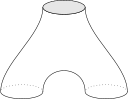
\includegraphics[width=3cm]{Pants.png}
    \label{fig: pair of pants}
    \caption{The pair of pants is a cobordism between $S^{1}$ and $S^{1}\sqcup S^{1}$.}
\end{figure}
This first arose in Pontryagin's study of manifolds and remains an active area of research to this day. Let $\Omega^{n}$ be the cobordism classes of $n$ manifolds. This naturally forms a monoid under the operation of disjoint union with identity element $\emptyset$. $\Omega^{n}$ can naturally be endowed with the structure of a group by noticing that $M\sqcup M$ is cobordant to $\emptyset$ by identifying the boundary of $M\times[0,1]$ yielding an $(n+1)$-manifold without boundary. \\\\
In the late 1980s, physicists were concerned about string theory, which encouraged the study of cobordisms that were treated as non-invertible transformations. This led to the definition of a cobordism category and topological quantum field theory. In particular, we define the bordism category as follows. 
\begin{definition}[$\Bord_{(n-1,n)}$]
    The category $\Bord_{(n-1,n)}$ has objects $(n-1)$-manifolds with morphisms cobordism and a composition law given by concatenation. 
\end{definition}
This definition leads to a problem. In concatenation, one must choose an appropriate open neighborhood of the boundaries of the $n$-manifolds. Different choices of open neighborhoods yield to different concatenated manifolds. In particular, the composition is not associative, but is associative up to diffeomorphism in a non-cannonical way. This leads us to believe that there is higher structure, in particular the structure of a symmetric monoidal category. 
\begin{definition}[Symmetric Monoidal Category]\label{def: symmetric monoidal category}
    A symmetric monoidal category $\Csf$ is a category $\Csf$ with a functor $\otimes:\Csf\times\Csf\to\Csf$ and an object $1_{\Csf}\in\Obj(\Csf)$ such that the following conditions are fulfiled: 
    \begin{enumerate}[label=(\alph*)]
        \item A natural isomorphism $1_{\Csf}\otimes 1_{\Csf}\to 1_{\Csf}$. 
        \item For all $A\in\Obj(\Csf)$, a natural isomorphisms $1_{\Csf}\otimes A\to A$ and $A\otimes 1_{\Csf}\to A$.
        \item For all $A,B\in\Obj(\Csf)$, a natural isomorphism $A\otimes B\to B\otimes A$. 
        \item For all $A,B,C\in\Obj(\Csf)$, a natural isomorphism $(A\otimes B)\otimes C\to A\otimes(B\otimes C)$. 
    \end{enumerate}
\end{definition}
One can check that $\sqcup$ defines an operation that satisfies the symmetric monoidal structure on $\Bord_{(n-1,n)}$ with $1_{\Bord_{(n-1,n)}}=\emptyset$. This leads to the definition of a topological quantum field theory. 
\begin{definition}[Topological Quantum Field Theory]
    A topological quantum field theory is a symmetric monoidal functor $\Bord_{(n-1,n)}\to\Csf$ for $\Csf$ a symmetric monoidal category. 
\end{definition}
For our discussion today, we consider $\Csf=\Vect_{\CC}$ yielding a functor $Z:\Bord_{(n-1,n)}\to\Vect_{\CC}$ taking an $(n-1)$-manifold $M$ to a $\CC$-vector space $Z(M)$ such that $Z(M_{1}\sqcup M_{2})\mapsto Z(M_{1})\otimes Z(M_{2})$ with unit $\emptyset$ in $\Bord_{(n-1,n)}$ to $Z(\emptyset)=\CC$. Suppose $N$ is an $n$-manifold defining a cobordism between $(n-1)$-manifolds $M_{1}$ and $M_{2}$. This yields a linear map of $\CC$-vector spaces $Z(M_{1})\to Z(M_{2})$. For $N$ a boundaryless $n$-manifold, $N$ is a cobordism between $\emptyset$ and $\emptyset$, hence $Z(N)$ is a map $\CC\to \CC$ by $1\mapsto\lambda$ for $\lambda\in\CC$. In such a case, it suffices to study this value $\lambda$. 
\\\\
Further restricting our case to oriented 1-manifolds up to cobordism by 2-manifolds, we consider the category $\Bord_{(1,2)}^{\mathrm{so}}$. Recall from a course in topology that a closed 1-manifold is the disjoint union of $S^{1}$s, and thus $Z(S^{1})$ is some $\CC$-vector space $V$. The upper half sphere gives a cobordism between $S^{1}$ and $\emptyset$, yielding a trace $V\to\CC$. In the case of cobordisms of 1-manifolds, there is a clear interpretation of the relavent topological quantum field theory. 
\begin{theorem}
    Symmetric monoidal functors $Z:\Bord_{(2,1)}^{\mathrm{so}}\to\Vect_{\CC}$ correspond to Frobenius algebras. 
\end{theorem}
Symmetric monoidal categories therefore define another model for $\infty$-categories that are used in the study of topological quantum field theories. These may seem idiosyncratic, but really are the most morally correct way to study these mathematical structures. Work in this area continues to this day, with a recent landmark result by Lurie in his solution of the Baez-Dolan Cobordism hypothesis, characterizing these cobordism categories by universal higher categorical structures. See the survey article by Freed \cite{Freed} for a brief overview and the papers by Ayala-Francis \cite{AyalaFrancis} and Grady-Pavlov \cite{GradyPavlov} for more information. 
\\\\
Let us now consider yet another approach to higher category theory. Let $\Csf$ be a category. Let's think about this category via the moduli space of functors to it. 
\begin{definition}[Maximal Groupoid]
    Let $\Csf$ be a category. The maximal groupoid in $\Csf$, denoted $\Csf^{\sim}$, is the maximal subcateory of $\Csf$ in which every morphism is an isomorphism. 
\end{definition}
Evidently $N\Csf^{\sim}$ is a Kan complex by Joyal's horn filling condition \Cref{thm: Joyal extension theorem}. This is the moduli space of objects of $\Csf$ in the sense that when we treat $N\Csf^{\sim}$ as a topological space, the connected components are isomorphism classes of objects. Similarly for $I$ an indexing category, $N(\Csf^{I})^{\sim}$ is the moduli space of $I$-diagrams in $\Csf$. We can probe this object by taking $I=[n]$ defining a functor $\DDelta\to N(\Csf^{\DDelta})^{\sim}$ by $[n]\mapsto N(\Csf^{[n]})^{\sim}$ valued in simplicial (topological) spaces. This led to the introduction of complete Segal spaces by Rezk. 
\begin{definition}[Segal Space; Rezk]\label{def: segal space}
    Let $X$ be a simplicial set. $X$ is a Segal space if for all $n$ if the Segal map $X^{\Delta_{n}}\to X^{I_{n}}$ induced by the spine inclusion $I_{n}\to\Delta^{n}$ given by 
    $$X_{n}\to\underbrace{X_{1}\times_{X_{0}}X_{1}\times_{X_{0}}\dots\times_{X_{0}}X_{1}}_{n\text{ times}}$$
    is an acyclic Kan fibration. 
\end{definition}
We can think of Segal spaces as a type of category whose objects are $X_{0}$ any two objects $A,B\in X_{0}$ we can define the space of maps between them as a pullback in the following diagram where $X\to X_{0}\times X_{0}$ is fibration 
$$% https://q.uiver.app/#q=WzAsNSxbMCwwLCJYXnsoQSxCKX0iXSxbMCwxLCIqIl0sWzIsMSwiWF97MH1cXHRpbWVzIFhfezB9Il0sWzIsMCwiWCJdLFswLDNdLFsxLDIsIihBLEIpIiwyXSxbMywyLCIoXFxsYW5nbGUwXFxyYW5nbGUsXFxsYW5nbGUxXFxyYW5nbGUpIl0sWzAsM10sWzAsMV1d
\begin{tikzcd}
	{X^{(A,B)}} && X \\
	{*} && {X_{0}\times X_{0}}
	\arrow["{(A,B)}"', from=2-1, to=2-3]
	\arrow["{(\langle0\rangle,\langle1\rangle)}", from=1-3, to=2-3]
	\arrow[from=1-1, to=1-3]
	\arrow[from=1-1, to=2-1]
\end{tikzcd}$$
and the space of map is denoted $X^{(A,B)}$. 
\begin{definition}[Complete Segal Space; Rezk]
    A segal space is complete if $X_{0}\to X_{1}^{\sim}$ is a homotopy equivalence of topological spaces where $X_{1}^{\sim}$ is the subset of isomorphisms in $X$. 
\end{definition}
Further work by Rezk and Joyal and Tierney relate complete Segal spaces to $\infty$-categories and quasicategories, respectively. 
\\\\
Returning to cobordism, we can let $X$ be a Segal space such that the $X_{0}$ correspond to closed $(n-1)$-manifolds. One can then show that 
$$X_{0}=\left\{S\subseteq\RR^{\infty}:S \text{ is a closed }(n-1)\text{-manifold}\right\}$$
and more generally
$$X_{n}=\left\{S\subseteq\RR^{\infty}\times\RR: S\text{ an }n\text{-manifold such that }\pi_{2}\text{ is proper and regular at }0,1,\dots,n\right\}.$$
Those more interested in this particular topic can refer to \cite{CalaqueScheimbauer}.
\newpage
\printbibliography
\end{document}